\documentclass[11pt,a4paper,chapterprefix=false,parskip=false]{scrreprt}

\usepackage[utf8]{inputenc}
\usepackage[T1]{fontenc}
\usepackage[english]{babel}
\usepackage[a4paper,top=2.45cm,bottom=2.55cm,left=2.55cm,right=2.55cm,headsep=0.45cm]{geometry}
\usepackage{lmodern}
\usepackage{microtype}
\usepackage{amsmath,amsfonts,amssymb}
\usepackage{graphicx}
\usepackage{caption}
\usepackage{subcaption}
\usepackage{float}
\usepackage{array}
\usepackage{longtable}
\usepackage{booktabs}
\usepackage{tabularx}
\usepackage{xcolor}
\usepackage{listings}
\usepackage{scrhack}
\usepackage[automark,headsepline]{scrlayer-scrpage}
\usepackage[toc]{appendix}
\usepackage[numbers]{natbib}
\usepackage{tikz}
\usetikzlibrary{arrows.meta, positioning, shapes.geometric, fit, calc}
\usepackage{pdfpages}
\usepackage{hyperref}
\usepackage{float}
\usepackage{booktabs}
\usepackage{tabularx}

%\usepackage{caption}
\usepackage{xcolor}

\newcommand{\atc}[1]{\textcolor{red}{#1}}

\KOMAoptions{numbers=noenddot}

\hypersetup{
    colorlinks=true,
    linkcolor=black,
    urlcolor=black,
    citecolor=black
}

\clearpairofpagestyles
\ihead{\headmark}
\ohead{\pagemark}
\automark[chapter]{chapter}
\renewcommand*{\chapterpagestyle}{plain}
\renewcommand*{\chapterformat}{\thechapter.\enskip}
\renewcommand*{\chaptermarkformat}{\thechapter.\enskip}
\setcounter{secnumdepth}{3}
\setcounter{tocdepth}{2}
\setlength{\parindent}{0pt}
\setlength{\parskip}{6pt plus 2pt minus 1pt}
\setlength{\headheight}{15pt}
\sloppy
\setkomafont{chapter}{\huge\bfseries}
\setkomafont{section}{\Large\bfseries}
\setkomafont{subsection}{\large\bfseries}
\RedeclareSectionCommand[beforeskip=0.75\baselineskip,afterskip=0.70\baselineskip]{chapter}
\RedeclareSectionCommand[beforeskip=1.15\baselineskip,afterskip=0.35\baselineskip]{section}
\RedeclareSectionCommand[beforeskip=0.70\baselineskip,afterskip=0.20\baselineskip]{subsection}

\lstset{
  basicstyle=\ttfamily\small,
  breaklines=true,
  frame=single,
  backgroundcolor=\color{gray!10}
}

\tikzset{
    pipeline/.style={draw=black!55, rounded corners=2pt, align=center, minimum height=8mm, text width=30mm, fill=gray!8},
    smallpipe/.style={draw=black!55, rounded corners=2pt, align=center, minimum height=7mm, text width=24mm, fill=gray!8},
    tensor/.style={draw=blue!60!black, fill=blue!10, rounded corners=1.5pt, minimum width=12mm, minimum height=24mm},
    feature/.style={draw=teal!60!black, fill=teal!10, rounded corners=1.5pt, align=center, minimum height=8mm, text width=25mm},
    modelblock/.style={draw=orange!70!black, fill=orange!12, rounded corners=1.5pt, align=center, minimum height=8mm, text width=25mm},
    statblock/.style={draw=purple!65!black, fill=purple!10, rounded corners=1.5pt, align=center, minimum height=8mm, text width=26mm},
    decision/.style={draw, diamond, aspect=2, align=center, inner sep=1pt, fill=gray!8},
    arrow/.style={-{Latex[length=2mm]}, thick, draw=black!70},
    thinarr/.style={-{Latex[length=1.7mm]}, draw=black!55},
    band/.style={draw=black!50, fill=black!4, rounded corners=2pt, inner sep=4pt}
}

\newcommand{\drawnetworkblock}[9]{
  % #1: unique name for coordinates
  % #2: x
  % #3: y
  % #4: dx (width/thickness)
  % #5: dy (height/spatial)
  % #6: dz (depth/temporal)
  % #7: base color
  % #8: text inside front face
  % #9: text below block
  \pgfmathsetmacro{\x}{#2}
  \pgfmathsetmacro{\y}{#3}
  \pgfmathsetmacro{\dx}{#4}
  \pgfmathsetmacro{\dy}{#5}
  \pgfmathsetmacro{\dz}{#6}
  
  \colorlet{tempcol}{#7}
  \colorlet{frontcol}{tempcol!85!black}
  \colorlet{topcol}{tempcol!55!white}
  \colorlet{sidecol}{tempcol!70!black}
  
  % Front face
  \fill[frontcol] (\x,\y) -- (\x+\dx,\y) -- (\x+\dx,\y+\dy) -- (\x,\y+\dy) -- cycle;
  \draw[draw=black!70, thin] (\x,\y) -- (\x+\dx,\y) -- (\x+\dx,\y+\dy) -- (\x,\y+\dy) -- cycle;
  
  % Top face (projected along 45 degrees, scaling factor 0.35)
  \fill[topcol] (\x,\y+\dy) -- (\x+\dx,\y+\dy) -- (\x+\dx+0.35*\dz,\y+\dy+0.35*\dz) -- (\x+0.35*\dz,\y+\dy+0.35*\dz) -- cycle;
  \draw[draw=black!70, thin] (\x,\y+\dy) -- (\x+\dx,\y+\dy) -- (\x+\dx+0.35*\dz,\y+\dy+0.35*\dz) -- (\x+0.35*\dz,\y+\dy+0.35*\dz) -- cycle;
  
  % Right face
  \fill[sidecol] (\x+\dx,\y) -- (\x+\dx+0.35*\dz,\y+0.35*\dz) -- (\x+\dx+0.35*\dz,\y+\dy+0.35*\dz) -- (\x+\dx,\y+\dy) -- cycle;
  \draw[draw=black!70, thin] (\x+\dx,\y) -- (\x+\dx+0.35*\dz,\y+0.35*\dz) -- (\x+\dx+0.35*\dz,\y+\dy+0.35*\dz) -- (\x+\dx,\y+\dy) -- cycle;
  
  % Define coordinates for external connections
  \coordinate (#1-frontcenter) at (\x+0.5*\dx, \y+0.5*\dy);
  \coordinate (#1-backcenter) at (\x+0.5*\dx+0.35*\dz, \y+0.5*\dy+0.35*\dz);
  \coordinate (#1-rightcenter) at (\x+\dx+0.175*\dz, \y+0.5*\dy+0.175*\dz);
  \coordinate (#1-leftcenter) at (\x+0.175*\dz, \y+0.5*\dy+0.175*\dz);
  \coordinate (#1-topcenter) at (\x+0.5*\dx+0.175*\dz, \y+\dy+0.175*\dz);
  \coordinate (#1-bottomcenter) at (\x+0.5*\dx+0.175*\dz, \y);
  
  \coordinate (#1-frontbottomleft) at (\x, \y);
  \coordinate (#1-fronttopleft) at (\x, \y+\dy);
  \coordinate (#1-frontbottomright) at (\x+\dx, \y);
  \coordinate (#1-fronttopright) at (\x+\dx, \y+\dy);
  \coordinate (#1-backbottomright) at (\x+\dx+0.35*\dz, \y+0.35*\dz);
  \coordinate (#1-backtopright) at (\x+\dx+0.35*\dz, \y+\dy+0.35*\dz);
  \coordinate (#1-backtopleft) at (\x+0.35*\dz, \y+\dy+0.35*\dz);
  \coordinate (#1-backbottomleft) at (\x+0.35*\dz, \y+0.35*\dz);
  
  % Text inside (front face)
  \node[text=black, font=\bfseries, align=center] at (\x+0.5*\dx, \y+0.5*\dy) {#8};
  
  % Caption below
  \node[text=black!90, font=\tiny, align=center, anchor=north] at (\x+0.5*\dx+0.175*\dz, \y) {#9};
}

\newcommand{\placeholderfigure}[3]{
\begin{figure}[H]
    \centering
    \fbox{\parbox{0.86\textwidth}{
        \centering
        \vspace{0.7cm}
        \textbf{#2}\\[0.2cm]
        #3
        \vspace{0.7cm}
    }}
    \caption{#3}
    \label{#1}
\end{figure}
}

\newcommand{\pipelinebox}[2]{
\begin{tikzpicture}[node distance=7mm]
    #2
\end{tikzpicture}
}

\newcommand{\panelimage}[3]{
    \begin{subfigure}{#1}
        \centering
        \includegraphics[width=\linewidth]{#2}
        \caption{#3}
    \end{subfigure}
}

\begin{document}
\pagenumbering{gobble}

\includepdf[pages=1,pagecommand={\thispagestyle{empty}}]{portada_cat.pdf}
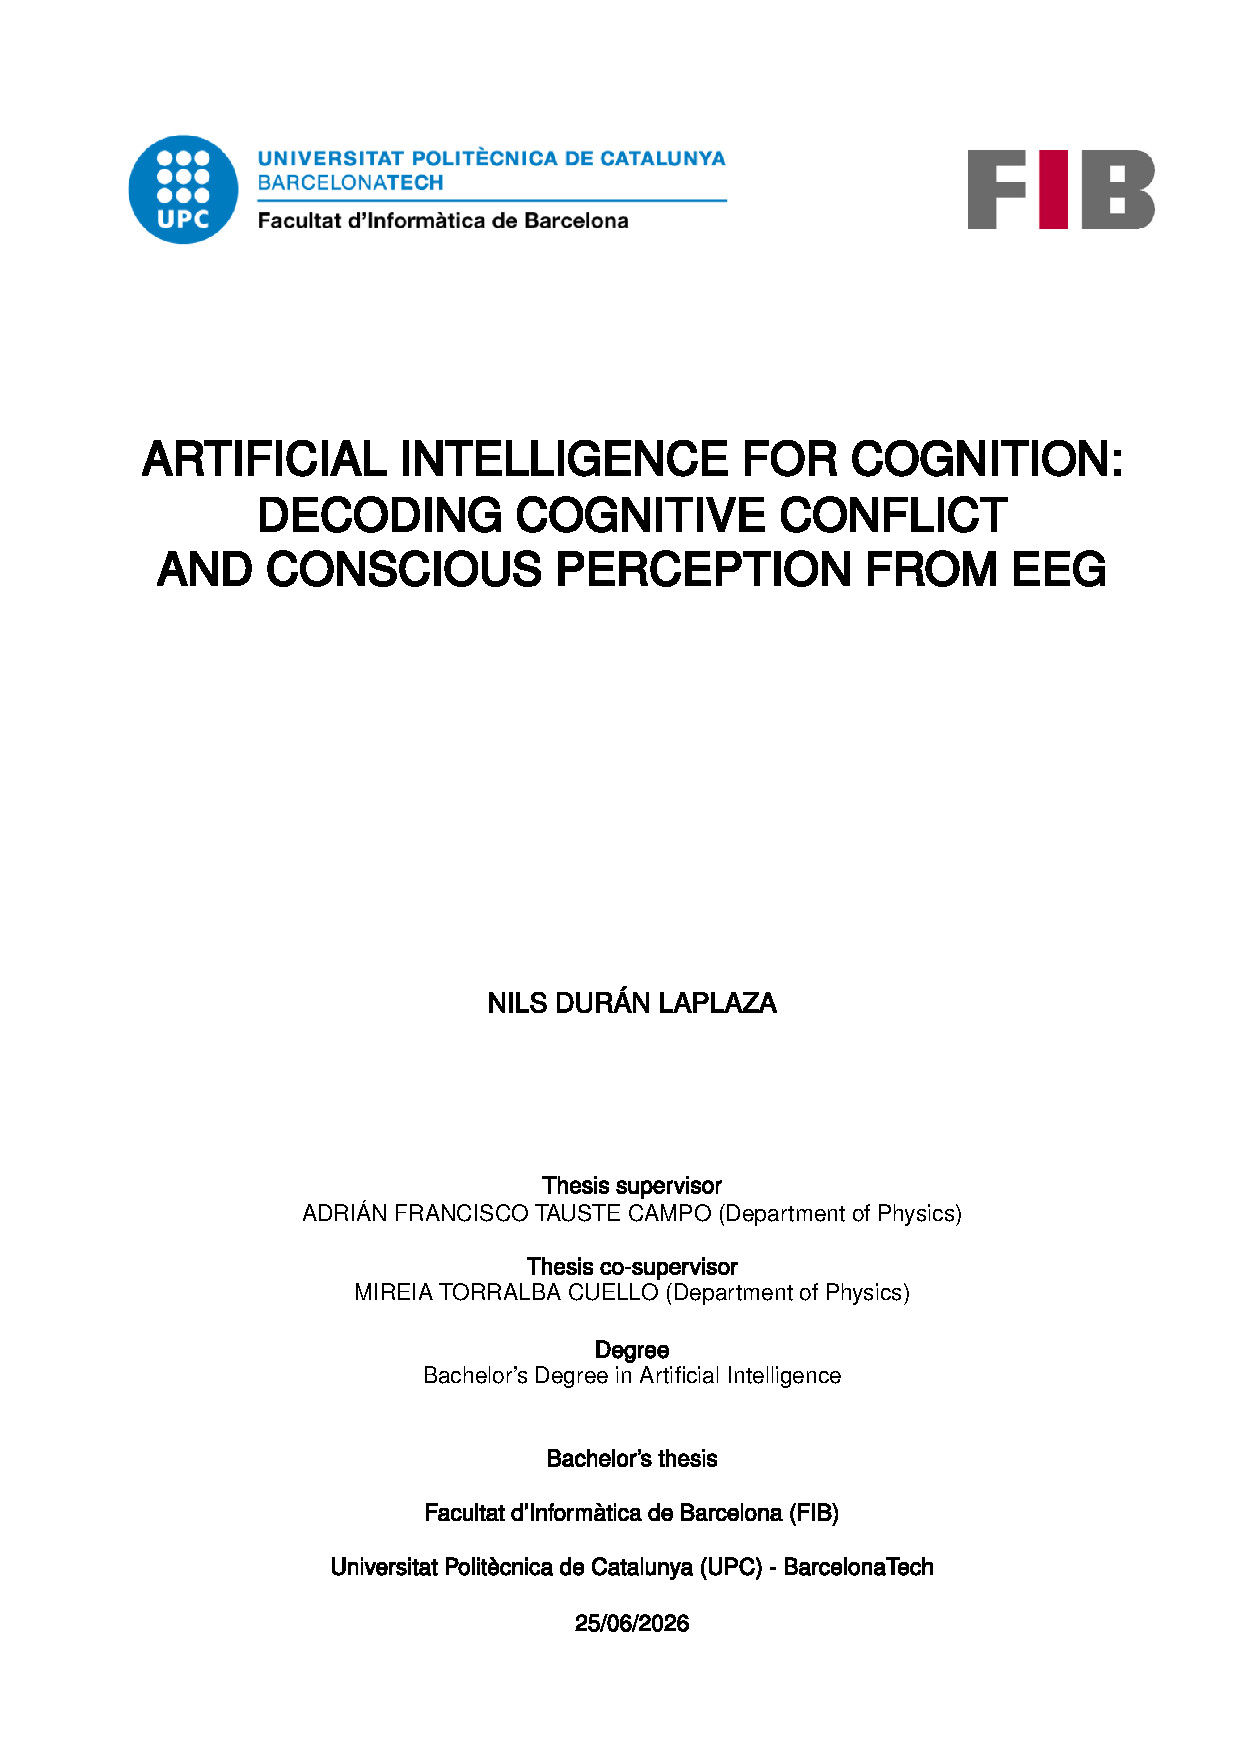
\includepdf[pages=1,pagecommand={\thispagestyle{empty}}]{portada_en.pdf}

\cleardoublepage
\pagenumbering{roman}
\pagestyle{plain}
\renewcommand*{\chapterpagestyle}{plain}

\chapter*{Abstract}
This thesis investigates whether electroencephalography (EEG) recorded during onset binocular rivalry contains decodable information about perceptual conflict. The work is based on the binocular-rivalry EEG dataset introduced by Drew and colleagues, where participants viewed dichoptic red/green stimuli and reported whether they perceived a green stimulus, a red stimulus, or a mixture of both. Machine learning is not treated as a generic prediction exercise. Instead, decoding is used as a controlled way to test whether conflict-related perceptual states leave weak but measurable signatures in single-trial EEG.

The thesis has four objectives: to replicate the main findings of the original paper, to extend its one-dimensional temporal clustering to two-dimensional spatiotemporal clustering over channels and time, to evaluate classical and modern EEG decoding models, and to interpret the resulting evidence in relation to binocular-rivalry theory and EEG validation limits. Two binary tasks structure the analysis. The first distinguishes compatible stimuli from incompatible stimuli when the participant reports one color only. The second focuses only on incompatible stimuli and distinguishes single-color reports from mixed reports.

The current results support a cautious positive answer for the contrast between compatible stimuli and incompatible stimuli with single-color reports. The signal is modest but structured: Riemannian covariance plus LDA is the most stable model family, alpha-band oscillatory features in occipital regions outperform the simple frontocentral theta baseline, and cluster analyses identify posterior alpha effects over broad post-stimulus windows. The mixed-versus-single-color contrast within incompatible stimulation is weaker and remains exploratory. The central methodological conclusion is that, for this small, noisy, subject-specific EEG dataset, carefully constrained classical EEG methods outperform or match larger neural models.

\textbf{Keywords:} binocular rivalry, EEG, oscillatory brain activity, perceptual conflict, machine learning, EEG foundation models.

\chapter*{Resum}
Aquesta tesi investiga si l'electroencefalografia (EEG) enregistrada durant un paradigma de rivalitat binocular d'inici conté informació descodificable sobre el conflicte perceptiu. El treball parteix del conjunt de dades EEG introduït per Drew i col·laboradors, en què participants observaven estímuls dicòptics vermells i verds i indicaven si percebien un estímul verd, un estímul vermell o una mescla entre tots dos. L'aprenentatge automàtic no s'utilitza com un exercici genèric de predicció, sinó com una eina per comprovar si els estats perceptius relacionats amb el conflicte deixen signatures febles però mesurables en l'EEG d'assaig únic.

El projecte es desenvolupa al voltant de quatre objectius: replicar els resultats principals del treball original, ampliar l'anàlisi estadística cap a clústers espaciotemporals en canals i temps, avaluar mètodes de descodificació clàssics i moderns, i interpretar els resultats en relació amb la teoria de rivalitat binocular i els límits pràctics de l'EEG. Les dues tasques principals són distingir, d'una banda, estímuls compatibles entre els dos ulls d'estímuls incompatibles quan el participant reporta un sol color i, de l'altra, dins dels estímuls incompatibles, respostes d'un sol color de respostes mixtes.

Els resultats actuals donen suport a una resposta positiva però prudent per al contrast entre estímuls compatibles i incompatibles amb respostes d'un sol color. El senyal és modest, però no sembla aleatori: la classificació riemanniana basada en covariàncies és la família de models més estable, les característiques d'activitat oscil·latòria alpha en regions occipitals superen la línia base theta en regions frontocentrals, i els clústers alpha posteriors apareixen en finestres posteriors a l'estímul. El contrast entre respostes mixtes i respostes d'un sol color dins dels estímuls incompatibles és més feble i continua sent exploratori. La conclusió metodològica central és que, en aquest conjunt de dades petit, sorollós i molt dependent del subjecte, els mètodes clàssics amb biaixos inductius adequats igualen o superen models neuronals més grans.

\textbf{Paraules clau:} rivalitat binocular, EEG, activitat cerebral oscil·latòria, conflicte perceptiu, aprenentatge automàtic, models fonamentals d'EEG.

\chapter*{Resumen}
Esta tesis investiga si la electroencefalografía (EEG) registrada durante un paradigma de rivalidad binocular de inicio contiene información descodificable sobre el conflicto perceptivo. El trabajo se basa en el conjunto de datos EEG introducido por Drew y colaboradores, en el que los participantes observaban estímulos dicópticos rojos y verdes e indicaban si percibían un estímulo verde, un estímulo rojo o una mezcla entre ambos. El aprendizaje automático se utiliza como herramienta de análisis, no como una simple competición predictiva.

El proyecto persigue cuatro objetivos: replicar los principales resultados del artículo original, extender el análisis de clústeres temporales unidimensionales hacia clústeres espaciotemporales en canales y tiempo, evaluar modelos de descodificación EEG clásicos y modernos, e interpretar los resultados dentro del marco de la rivalidad binocular y la validación de señales EEG. Las dos tareas principales son distinguir, por un lado, estímulos compatibles entre los dos ojos de estímulos incompatibles cuando el participante informa de un solo color y, por otro, dentro de los estímulos incompatibles, respuestas de un solo color de respuestas mixtas.

Los resultados actuales apoyan una respuesta positiva pero prudente para el contraste entre estímulos compatibles e incompatibles con respuestas de un solo color. La señal es débil, pero estructurada: la clasificación riemanniana basada en covarianzas es la familia de modelos más estable, las características de actividad oscilatoria alpha en regiones occipitales superan la línea base theta en regiones frontocentrales, y los clústeres alpha posteriores aparecen en ventanas posteriores al estímulo. El contraste entre respuestas mixtas y respuestas de un solo color dentro de los estímulos incompatibles es más difícil y debe interpretarse como exploratorio. La conclusión metodológica principal es que, en este conjunto de datos EEG pequeño y ruidoso, los métodos clásicos con sesgos inductivos adecuados igualan o superan modelos neuronales de mayor capacidad.

\textbf{Palabras clave:} rivalidad binocular, EEG, actividad cerebral oscilatoria, conflicto perceptivo, aprendizaje automático, modelos fundacionales de EEG.

\chapter*{Agraïments}
M'agradaria expressar el meu agraïment a totes les persones que han fet possible aquest treball.

En primer lloc, als meus dos tutors, la Mireia Torralba i l'Adrià Tauste. Veure dos científics treballant plegats, intercanviant idees i refinant-les de manera iterativa ha estat una font d'inspiració i m'ha empès a donar el millor de mi mateix. Em sento molt afortunat d'haver pogut beneficiar-me de la seva generositat, tant pel que fa al temps com al talent i la implicació que m'han dedicat.

També voldria agrair a la meva família i als meus amics el seu suport i interès al llarg d'aquest treball, compartint amb mi tant els triomfs com les dificultats del camí.

Aquest TFG posa punt final a una etapa, però també voldria reconèixer tots els mestres i educadors que m'han acompanyat al llarg dels anys. En especial, l'Eli González i en David López-Val, per haver confiat en mi abans que jo mateix ho fes.

\tableofcontents

\cleardoublepage
\pagenumbering{arabic}
\pagestyle{scrheadings}
\renewcommand*{\chapterpagestyle}{scrheadings}

\chapter{Introduction}
\label{chap:introduction}

\section{Context}
The brain receives vast amounts of sensory information every moment, but only a fraction of it is relevant for conscious processing. The mystery of how our two eyes generate a single, stable mental image has fascinated thinkers for millennia, with early discussions appearing in the works of Aristotle, Ptolemy, and Ibn al-Haytham~\citep{biasiucci_electroencephalography_2019}. However, it was not until the nineteenth century, with Wheatstone's invention of the stereoscope, that binocular rivalry was formally isolated and studied as a laboratory paradigm~\cite{biasiucci_electroencephalography_2019}.


\textbf{Binocular rivalry} (BR) is a visual phenomenon that occurs when incompatible images are presented simultaneously to the two eyes~\cite{blake_can_2014}. Instead of perceiving a stable fusion of the two images,  observers usually report alternations between them (first one, then the other) or a mixed percept in which both are partially visible~\citep{blake_can_2014, wade_early_2013}.


When conflicting visual representations compete for selection, central executive neural networks are engaged to detect and resolve this competition~\citep{drew_conflict_2022}. This makes BR an ideal benchmark for evaluating statistical and machine learning frameworks capable of capturing dynamic, non-stationary neural states.


\textbf{Electroencephalography} (EEG) provides a non-invasive method to measure electrical activity at the scalp with high temporal resolution but lower spatial resolution than other neural imaging techniques like fMRI~\cite{biasiucci_electroencephalography_2019}. Contrary to popular belief, EEG does not measure the current of individual neurons, but instead reflects postsynaptic potentials from synchronized groups of neurons~\cite{biasiucci_electroencephalography_2019, nunez_electric_2006}. This neural activity is characterized by rhythmic oscillations grouped into specific frequency bands, which can be informative about cognitive processes when interpreted at the appropriate sensor level. In the context of binocular rivalry and conflict monitoring, two primary spectral components are highly relevant: fronto-medial theta activity ($4-8$ Hz) and parieto-occipital alpha activity ($8-12$ Hz)~\cite{drew_neural_nodate, torralba_cuello_alpha_2022}.


Prior literature links fronto-medial theta power to cognitive control and sensory conflict monitoring, but this should be treated as a sensor-level association rather than direct evidence for a specific cortical source~\cite{drew_conflict_2022, drew_binocular_2026, nunez_electric_2006}. Parieto-occipital alpha power is linked with visual attention, and alpha suppression is often interpreted as reduced inhibition of task-relevant visual input~\cite{torralba_cuello_alpha_2022}.


While classical methods are useful for analyzing group-level, condition-averaged representations, they often fail to capture the complexity of trial-by-trial variability in EEG recordings. \textbf{Machine learning} applied to EEG data addresses this limitation by introducing predictive modeling, transforming the analytical focus from descriptive group statistics to single-trial classification. However, decoding neural signals requires specialized architectures capable of handling a low signal-to-noise ratio, strong spatial and temporal correlations, and the multi-dimensional structure of the data. To address these challenges, advanced decoding approaches treat EEG recordings as complex spatiotemporal patterns, leveraging mathematical transformations or specialized network structures to extract robust features from multi-channel time series.

\section{Motivation}
This bachelor's thesis builds on the onset BR EEG work of Drew, Torralba, et al.~\citep{drew_binocular_2026, drew_conflict_2022}. Their work links visual rivalry to cognitive conflict and reports modulations of fronto-medial theta and parieto-occipital alpha activity. Its theta and alpha interpretation motivates both the replication analysis and the later decoding models.

While the original study characterizes temporal dynamics, it does not explore a data-driven framework to locate where these spectral effects are strongest across the entire scalp, since it is based on domain-knowledge hypotheses. Second, because it relies on condition averages, it remains unknown whether these neural signatures carry enough information to decode a participant's perceptual state on a single-trial basis.

\section{Objectives}
This work has four main objectives, which are:
\begin{enumerate}
    \item Replicate the main theta and alpha findings of the original binocular-rivalry EEG paper.
    \item Extend the statistical analysis from one-dimensional temporal clustering to two-dimensional spatiotemporal clustering over channels and time.
    \item Evaluate whether single-trial EEG can decode the presence of visual conflict as well as the stability of conflict resolution using classical, Riemannian, deep-learning, and pretrained EEG models.
    \item Interpret the results through accuracy, statistics, topographies, temporal windows, spectral information, subject variability, and model attribution.
\end{enumerate}

The rest of the thesis follows the logic of that progression. Chapter~\ref{chap:background} introduces binocular rivalry, EEG, and machine learning for EEG. Chapter~\ref{chap:data} describes the dataset and dataset analysis, because the later models can only be interpreted correctly if class imbalance, subject bias, and session structure are understood first. Chapter~\ref{chap:clustering} presents the spatiotemporal clustering analysis, moving from paper-style replication to two-dimensional channel-time statistics and subject-level Jaccard variability. Chapter~\ref{chap:methods} describes the decoding methods, from transparent linear baselines to Riemannian covariance and deep architectures. Chapter~\ref{chap:results} reports the decoding results and compares the model families. Chapter~\ref{chap:discussion} draws the scientific and methodological interpretation together. Chapter~\ref{chap:ethics} addresses privacy, responsible claims, and reproducibility, and Chapter~\ref{chap:conclusions} closes with the main answers and future work.

\chapter{Theoretical Background}
\label{chap:background}

\section{Binocular Rivalry}
Binocular rivalry is useful for studying visual perception because it separates the physical stimulus from conscious experience. When each eye receives a different and incompatible image, perception does not usually settle into a single fused interpretation. Instead, observers experience alternating periods in which one image dominates, interleaved with moments in which both images are partially visible as a mixed or piecemeal percept \citep{blake_can_2014, arnold_why_2011}. The external stimulation can remain unchanged while subjective experience changes, which makes rivalry a controlled way to study how the visual system resolves competing sensory interpretations.

Rivalry is not only a switch between two clean perceptual states. Mixed percepts are a genuine part of the phenomenon, and their frequency depends on stimulus properties, attention, and individual differences \citep{levelt_1965, blake_can_2014}. This matters for interpretation because a mixed report can reflect partial dominance, spatial fragmentation, rapid alternation, uncertainty, or some combination of these experiences. Treating mixed perception as simple noise would therefore miss an important part of rivalry dynamics.

The timing of rivalry also has a characteristic structure. Dominance episodes are variable, but their durations are not arbitrary: many studies describe them as right-skewed, gamma-like distributions, with many short or medium dominance periods and fewer long ones \citep{levelt_1965, blake_can_2014}. Any neural or computational account of rivalry must therefore explain both the content of perceptual dominance and the stochastic timing of transitions between perceptual states.

\begin{figure}[H]
    \centering
    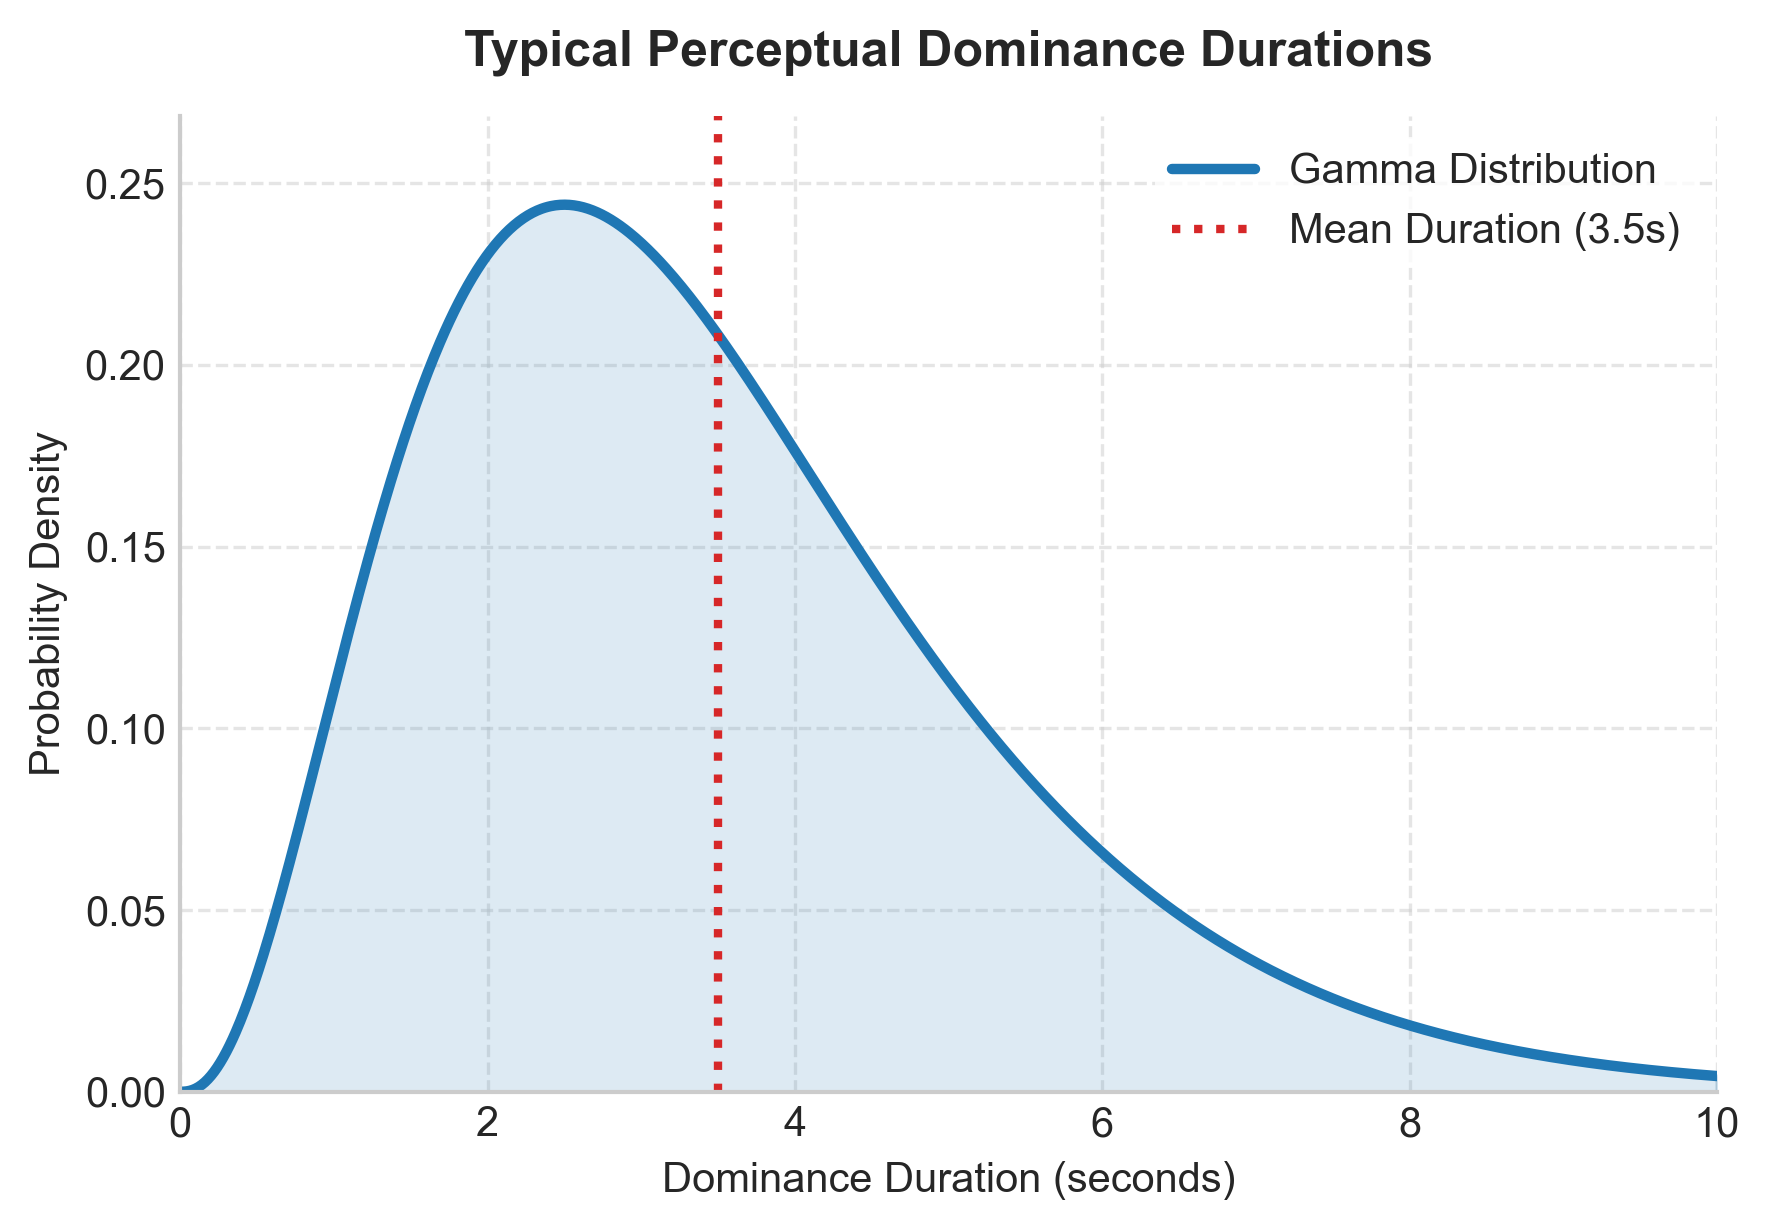
\includegraphics[width=0.5\linewidth]{images/gamma.png}
    \caption{Schematic distribution of typical perceptual dominance durations in binocular rivalry. Dominance episodes are variable and typically right-skewed, often described as gamma-like in the rivalry literature \cite{manousakis_when_2010}.}
    \label{fig:rivalry-gamma-durations-background}
\end{figure}

\section{Electroencephalography}
EEG records voltage fluctuations at the scalp generated mainly by the summed synaptic activity of large neuronal populations \citep{biasiucci_electroencephalography_2019, nunez_electric_2006}. Its main advantage is temporal resolution: EEG can follow neural dynamics at the millisecond scale. Its main limitation is spatial ambiguity. A scalp electrode does not measure a single cortical source. The recorded signal is shaped by volume conduction, reference choice, electrode placement, artifacts, and preprocessing. For that reason, scalp topographies are interpreted as sensor-level evidence, not as direct anatomical maps.

EEG activity is often described in terms of oscillatory components. A complex signal can be decomposed into frequency ranges such as delta, theta, alpha, beta, and gamma, although these bands are conventions rather than strict biological categories \citep{cohen_analyzing_2014}. Oscillatory power is useful because cognitive and perceptual processes often modulate specific frequency ranges. In visual perception, alpha activity over occipital and parietal regions is commonly linked to visual engagement, attention, and inhibition of task-irrelevant input \citep{torralba_cuello_alpha_2022}. Fronto-medial theta activity is often associated with conflict monitoring and cognitive control \citep{drew_conflict_2022}.

These rhythms are relevant to binocular rivalry because perceptual competition involves sensory selection and conflict between incompatible interpretations. Previous work has linked rivalry and perceptual conflict to changes in fronto-medial theta and parieto-occipital alpha activity \citep{drew_conflict_2022, drew_binocular_2026}. This does not mean that theta is simply ``conflict'' or alpha is simply ``inhibition'': the same band can reflect different mechanisms depending on region, task, and analysis method. Still, the theta--alpha framework gives a biologically grounded starting point for analyzing rivalry-related EEG.

Oscillatory EEG analysis usually examines how signal power is distributed across frequencies and changes over time. Time-frequency methods are especially relevant here because they localize oscillatory activity within approximate time windows, at the cost of a trade-off between temporal and frequency precision \citep{cohen_analyzing_2014}. Time windows and cluster boundaries should therefore be interpreted as approximate regions of evidence, not exact neural onset times.

\section{Machine Learning Applied to EEG}
Traditional EEG analyses often ask whether two conditions differ on average. Single-trial decoding asks a stricter question: does an individual EEG trial contain enough information to infer the condition or perceptual state that produced it? A pattern that only appears after averaging many trials may be scientifically meaningful but too weak or unstable to classify at the single-trial level \citep{lotte_review_2018}.

EEG decoding is difficult because the signal-to-noise ratio is low, trials from the same participant are correlated, neighboring electrodes are not independent, and slow changes in fatigue, attention, or electrode impedance can create temporal dependence across a recording session. Standard random cross-validation can therefore be misleading: if similar trials from the same subject or session appear in both training and validation sets, a classifier may learn subject identity or session drift rather than the intended neural contrast \citep{white_k-fold_2023, del_pup_role_2025}. Careful validation design is therefore part of the scientific method, not a secondary technical detail.

Several model families are commonly used for EEG decoding. Linear classifiers and support vector machines work well with compact, interpretable features. Riemannian methods represent trials through covariance matrices and often perform well on small EEG datasets \citep{lotte_review_2018, tibermacine_riemannian_2024}. Deep architectures such as EEGNet learn temporal and spatial filters directly from data \citep{lawhern_eegnet_2018}. Graph neural networks model the electrode montage as a spatial graph \citep{klepl_graph_2024}, and recent pretrained EEG foundation models transfer representations learned from large multi-dataset corpora \citep{jiang_large_2024, yang_are_2025}. These approaches differ in accuracy, data requirements, computation, and interpretive caution.

Statistical controls remain essential even when machine learning is used. Permutation testing estimates chance performance empirically by repeatedly shuffling labels and recomputing the analysis \citep{maris_nonparametric_2007}. Cluster-based permutation testing applies a similar logic to sensor-time maps by grouping neighboring significant samples and comparing cluster mass against a null distribution. Attribution methods can help diagnose which sensors, time points, or features influenced a trained model, but they should not be mistaken for source localization \citep{kobler_interpretation_2021, zhou_interpretable_2023, montavon_methods_2018, sundararajan_axiomatic_2017}. Interpretation is strongest when decoding, statistics, spectral information, topographies, and subject-level variability point in a coherent direction.


\chapter{Dataset and Experimental Context}
\label{chap:data}

\section{Experimental Task and Labels}

This chapter describes the dataset in the order in which it matters for the thesis: first the task and its labels, then the recording and preprocessing, and only afterwards the empirical structure of the available trials. The data come from the onset binocular rivalry experiment reported by \citeauthor{drew_binocular_2026} \citep{drew_binocular_2026}. The goal of this section is not to reproduce every technical detail of the source experiment, but to make the task understandable: what participants saw, what they were asked to do, and how their responses become the classes used in the decoding analyses.

In each trial, participants viewed red and green oriented Gabor patches through a mirror stereoscope, which allowed the experiment to control the image shown to each eye. Some trials presented compatible input: both eyes received the same-colored stimulus. Other trials presented incompatible input: one eye received a red stimulus and the other a green stimulus, creating the conditions for binocular rivalry. From the participant's point of view, the task was deliberately simple. They looked at the stimulus while it was on the screen, made no response during the viewing period, and then reported what they had perceived only after the stimulus had disappeared.

Each trial followed a fixed sequence: a blank fixation period, a smooth fade-in of the stimulus, a presentation interval, a short variable jitter, and finally a delayed response screen. This delayed response is important because the main EEG window analyzed in the thesis corresponds to stimulus viewing rather than button pressing. The trial structure is shown in Figure~\ref{fig:trial-timeline}.

\begin{figure}[H]
    \centering
    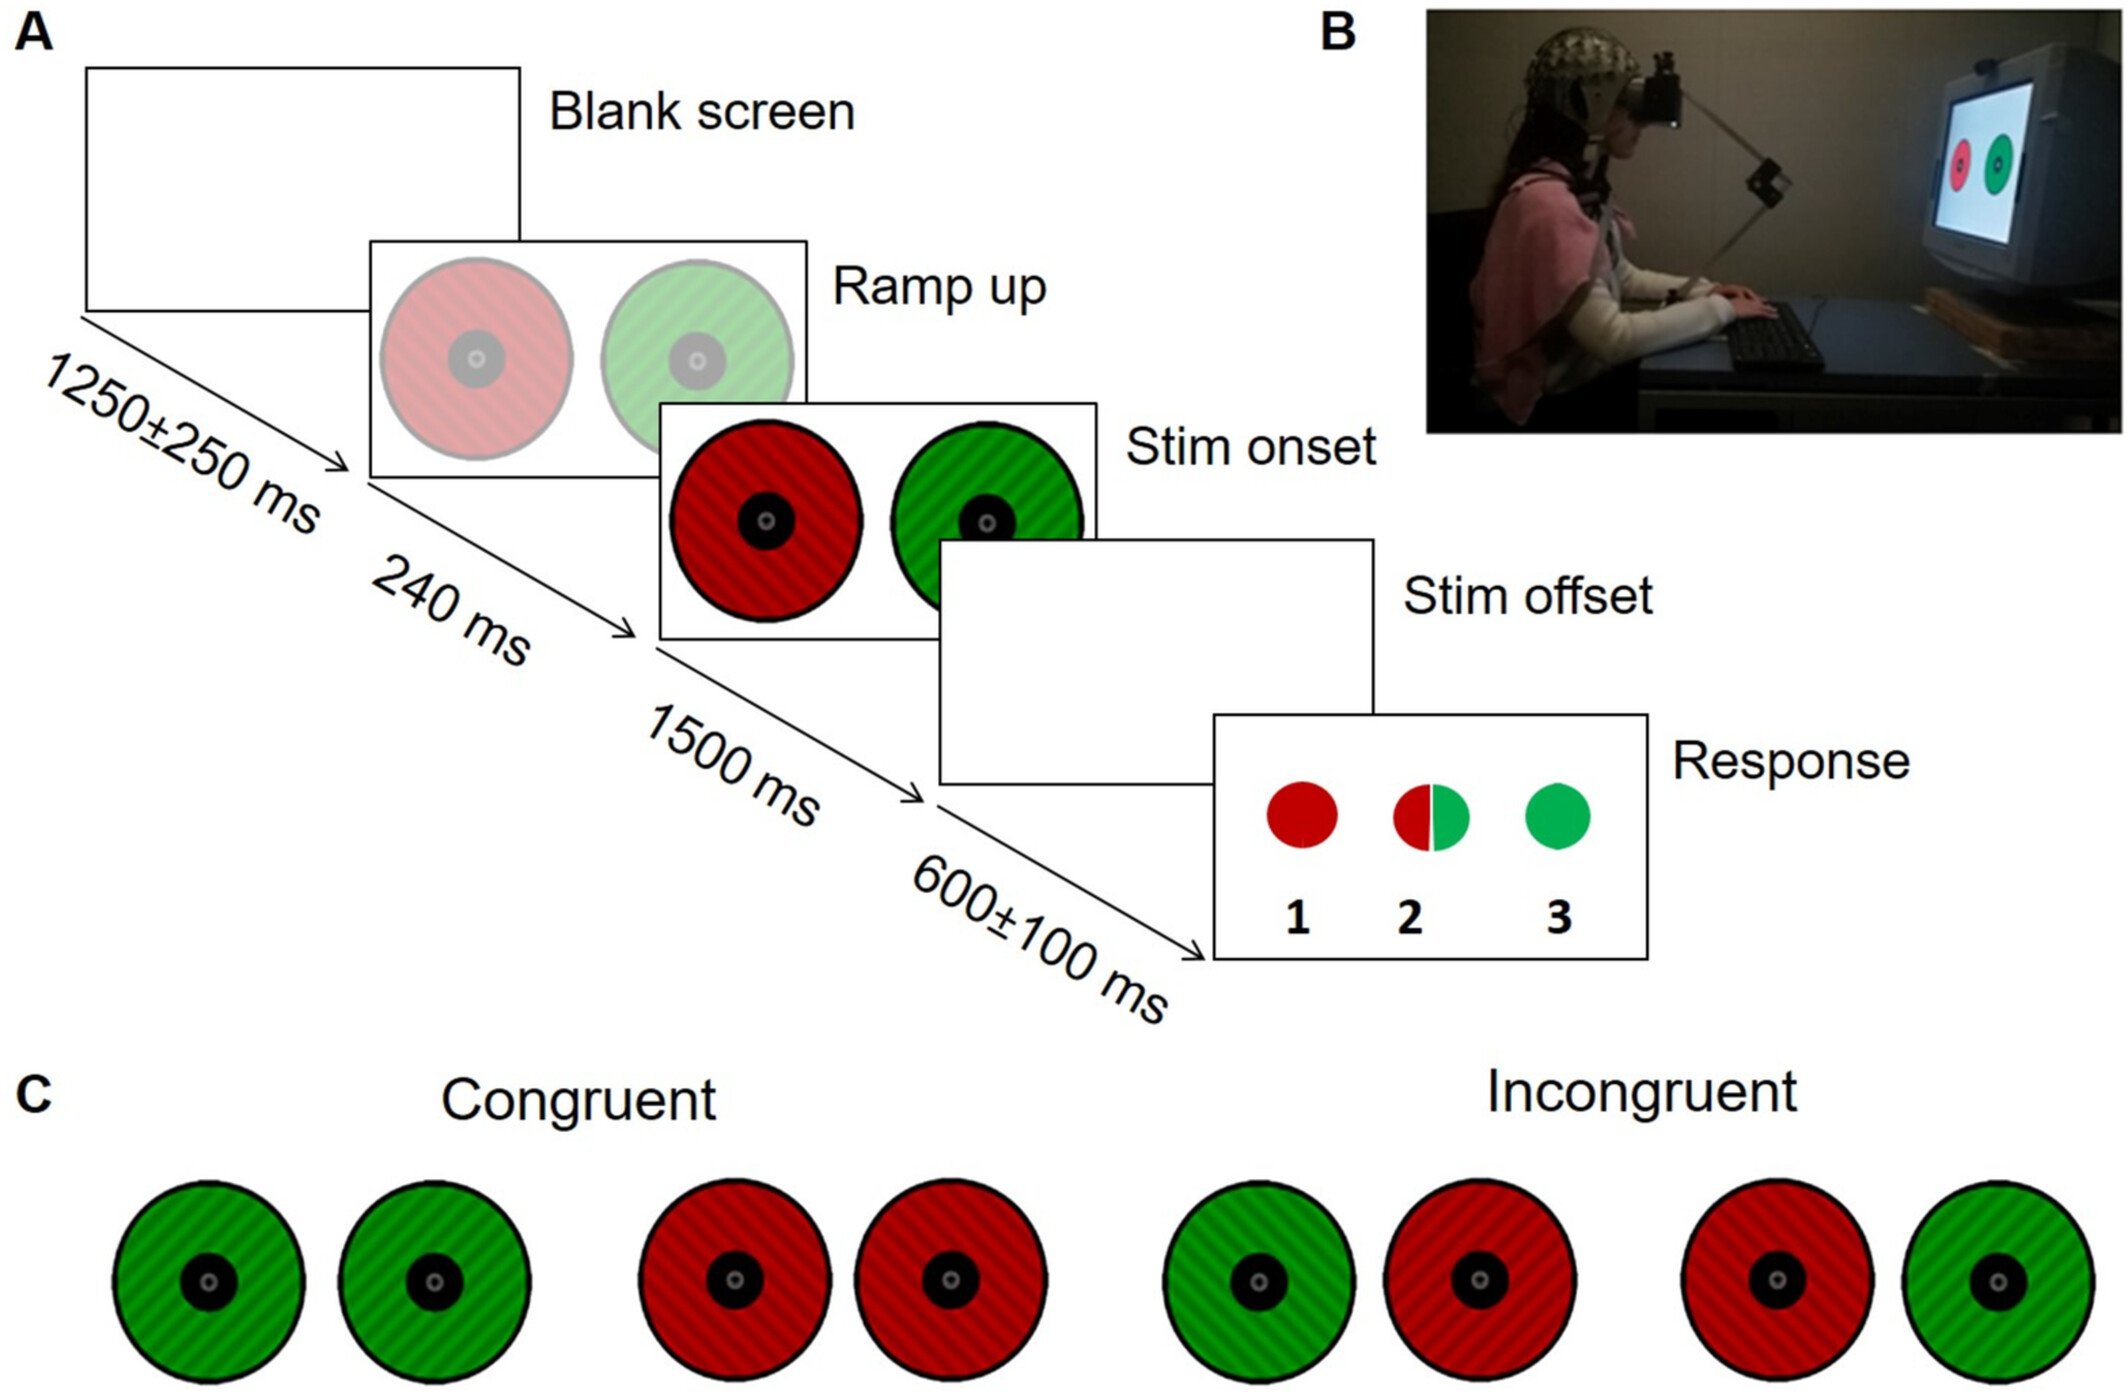
\includegraphics[width=0.92\textwidth]{images/experimental_paradigm.png}
    \caption{Onset-rivalry trial timeline. Each trial begins with a blank fixation screen, followed by a fade-in, a stimulus presentation interval (the main analysis window), a jitter, and finally the delayed response screen where participants reported their perception.}
    \label{fig:trial-timeline}
\end{figure}

On each trial, participants reported whether they had perceived green, red, or a mixture of the two. They did not report the categories used later in the thesis. The labels \textbf{Congruent (C)}, \textbf{Incongruent-Pure (IP)}, and \textbf{Incongruent-Mixed (IM)} are analytical labels assigned afterwards by combining the physical stimulus configuration with the behavioral report:

\begin{itemize}
    \item \textbf{Congruent (C):} Compatible binocular input; participant reports a single pure color. These are the baseline, lower-conflict trials.
    \item \textbf{Incongruent-Pure (IP):} Incompatible binocular input (rivalry-inducing), but the participant reports a single pure color --- one image dominated completely.
    \item \textbf{Incongruent-Mixed (IM):} Incompatible binocular input, and the participant reports a mixture --- both colors were partly visible.
\end{itemize}

\begin{figure}[H]
    \centering
    \resizebox{0.94\textwidth}{!}{%
        \begin{tikzpicture}[font=\small, >=Latex]
            \node[draw, rounded corners=3pt, fill=teal!10, minimum width=34mm, minimum height=13mm, align=center] (stim) at (0,0) {Stimulus\\configuration};
            \node[draw, rounded corners=3pt, fill=blue!10, minimum width=34mm, minimum height=13mm, align=center] (report) at (4.2,0) {Participant\\report};
            \node[draw, rounded corners=3pt, fill=yellow!18, minimum width=40mm, minimum height=13mm, align=center] (label) at (8.7,0) {Analysis\\label};
            \draw[->, thick] (stim) -- (report);
            \draw[->, thick] (report) -- (label);

            \node[align=center, font=\scriptsize, text width=33mm] at (0,-1.15) {compatible\\or incompatible};
            \node[align=center, font=\scriptsize, text width=33mm] at (4.2,-1.15) {green, red,\\or mixture};
            \node[align=center, font=\scriptsize, text width=42mm] at (8.7,-1.15) {C, IP, or IM\\assigned after the task};
        \end{tikzpicture}
    }
    \caption{Construction of the labels used in the thesis. Participants reported perceived color or mixture; C, IP, and IM are analysis labels derived afterwards from the report and the stimulus configuration.}
    \label{fig:label-construction}
\end{figure}

These three labels define the two binary classification tasks used later in the thesis. The first, \textbf{C vs IP}, contrasts congruent trials against incongruent trials when the participant reported one color only. Because both classes involve a single-color report, this comparison keeps the report type similar while changing whether the visual input was physically conflicting. The second, \textbf{IM vs IP}, compares two possible outcomes of the same incompatible input: a mixed report versus a single-color report. This contrast is scientifically important but harder to interpret because a ``mixed'' report can cover several subjective experiences, from a spatial mixture to rapid alternation or uncertainty.


\section{Experimental Setup}
\label{sec:experimental-setup}
Only the setup details needed to interpret the present analyses are summarized here. Full apparatus and acquisition details are available in the source study \citep{drew_binocular_2026}.

\paragraph{Apparatus and Stimuli}
Participants viewed red and green oriented Gabor patches through a mirror stereoscope, so the image shown to each eye could be controlled independently. This is the essential feature of the setup: some trials presented compatible input to the two eyes, while others presented incompatible red--green input and therefore induced rivalry.

\paragraph{Luminance Calibration}
Red and green luminance were calibrated for each participant using heterochromatic flicker photometry \citep{cavanagh_equiluminance_1987}. This matters here because the later exploratory analysis shows a red-report bias. The most relevant interpretation is not that the task was uncontrolled, but that the calibration may have slightly overcorrected the red--green balance, leaving red percepts somewhat favored in the available behavioral data.

\paragraph{Experimental Procedure}
The task was organized in repeated blocks of short trials. Participants viewed the stimulus without responding, and only after the stimulus disappeared did they report whether they had perceived green, red, or a mixture. This delayed response design is the methodological detail that matters for the EEG analyses, because it separates the stimulus-viewing window from the later motor response.

\paragraph{EEG Recording Setup}
EEG was recorded with a 64-electrode active system arranged according to the international 10-10 layout. The working dataset used in this thesis contains 60 EEG electrodes sampled at 500 Hz. Vertical and horizontal electrooculogram channels were recorded to detect blinks and eye movements, which are important because ocular events can alter perception or contaminate visual EEG responses for reasons unrelated to binocular conflict.


\section{Preprocessing Pipeline}
\label{sec:dataset-preprocessing}
The EEG available for this thesis had already been preprocessed in the source workflow using FieldTrip and MATLAB. Bad channels were identified and interpolated, and contaminated epochs were rejected after visual inspection. VEOG and HEOG channels were used to detect blinks and eye movements. Affected trials were rejected and the dataset should be described as preprocessed EEG, with EOG-informed artifact monitoring and epoch rejection.

The broad exploratory analysis includes 47 subjects. The final working montage contains 60 EEG channels, sampled at 500 Hz, and spans approximately 3.5 seconds around the trial event. The decoding analyses crop the main working window to 0--1.5 s unless a specific model requires another window or sampling rate.

The project pipeline starts from these preprocessed epochs. It selects the subjects and event codes needed for each binary task, crops the analysis window, optionally resamples or prepares model-specific representations, balances classes within subject, and applies scaling inside the training fold. The important validation principle is that any transformation with learned parameters must be fitted on the training data only and then applied to validation data, avoiding leakage from evaluation trials.

The same base pipeline supports several representations. Logistic regression receives compact band-envelope features, Riemannian methods receive covariance matrices, SVC models receive cluster-restricted summaries, and deep models receive tensors, graphs, patches, or resampled inputs depending on their architecture. Thus preprocessing is not only a technical preliminary: it defines what information each model is allowed to use.


\begin{figure}[H]
    \centering
    \resizebox{\textwidth}{!}{%
        \begin{tikzpicture}[font=\small, >=Latex]
            % Preprocessed epochs tensor block (3D)
            \drawnetworkblock{raw_tensor}{-1.2}{1.0}{0.8}{1.6}{1.2}{blue!20}{\tiny EEG}{Preprocessed\\Epochs\\$N \times C \times T$}

            % Draw irregular EEG-like traces on the tensor face.
            \draw[blue!65!black, very thin] (-1.1,1.26) -- (-1.06, 1.31) -- (-1.02, 1.19) -- (-0.98, 1.27) -- (-0.94, 1.17) -- (-0.90, 1.34) -- (-0.86, 1.22) -- (-0.82, 1.38) -- (-0.78, 1.19) -- (-0.74, 1.29) -- (-0.70, 1.21) -- (-0.66, 1.39) -- (-0.62, 1.18) -- (-0.58, 1.33) -- (-0.54, 1.27) -- (-0.50, 1.34);
            \draw[blue!65!black, very thin] (-1.1,2.28) -- (-1.06, 2.33) -- (-1.02, 2.21) -- (-0.98, 2.30) -- (-0.94, 2.19) -- (-0.90, 2.36) -- (-0.86, 2.24) -- (-0.82, 2.41) -- (-0.78, 2.22) -- (-0.74, 2.32) -- (-0.70, 2.24) -- (-0.66, 2.38) -- (-0.62, 2.20) -- (-0.58, 2.33) -- (-0.54, 2.27) -- (-0.50, 2.33);

            % Main flow blocks (flat but colored)
            \drawnetworkblock{events}{1.0}{1.3}{2.2}{1.0}{0.0}{teal!15}{\scriptsize Event Filter}{Keep C, IP, IM trials}
            \drawnetworkblock{crop}{4.0}{1.3}{2.2}{1.0}{0.0}{teal!15}{\scriptsize Crop Window}{Select 0--1.5 s epoch}
            \drawnetworkblock{balance}{7.0}{1.3}{2.2}{1.0}{0.0}{teal!15}{\scriptsize Class Balance}{Undersample majority}

            % Group Frame around representation variants
            \draw[draw=black!40, dashed, rounded corners=3pt, fill=black!3] (0.1, -3.4) rectangle (9.3, -0.6);
            \node[anchor=south, font=\scriptsize\bfseries\color{black!80}] at (4.7, -0.6) {Representation Variants};

            % Representation Variants Blocks (3D)
            % 1. Broadband tensor
            \drawnetworkblock{broad}{0.5}{-2.6}{1.1}{1.2}{0.6}{blue!15}{\tiny Broad}{1--40 Hz Tensor\\$C \times T$}

            % 2. Envelopes
            \drawnetworkblock{envelope}{2.8}{-2.6}{1.1}{1.2}{0.6}{purple!15}{\tiny Env}{Theta/Alpha\\Hilbert Mean}
            % Draw a signal + envelope inside envelopes
            \draw[red!80, thick, dash pattern=on 2pt off 1pt] (2.9,-1.82) .. controls (3.03,-1.55) and (3.18,-1.52) .. (3.30,-1.88)
            .. controls (3.39,-2.14) and (3.48,-1.92) .. (3.55,-1.72);
            \draw[black!65, very thin] (2.9,-2.00) .. controls (2.94,-1.82) and (2.98,-2.12) .. (3.03,-1.75)
            .. controls (3.08,-1.45) and (3.12,-2.05) .. (3.17,-1.66)
            .. controls (3.22,-2.24) and (3.27,-1.72) .. (3.32,-2.04)
            .. controls (3.39,-1.55) and (3.45,-2.12) .. (3.52,-1.80);

            % 3. Covariance
            \drawnetworkblock{cov}{5.1}{-2.6}{1.1}{1.2}{0.6}{orange!15}{\tiny Cov}{OAS tangent\\space matrices}
            % Draw correlation grid
            \foreach \xidx in {0,1,2} \foreach \yidx in {0,1,2} {
                    \pgfmathsetmacro{\op}{0.15 + 0.65*rnd}
                    \fill[orange!80, opacity=\op] (5.2+\xidx*0.28, -2.5+\yidx*0.32) rectangle ++(0.24,0.28);
                }

            % 4. Spatial Graph
            \drawnetworkblock{graph}{7.4}{-2.6}{1.1}{1.2}{0.6}{green!15}{\tiny Graph}{Spatial connectivity\\patches}
            % Draw nodes & edges
            \fill[teal] (7.6, -2.1) circle (1.2pt) (7.8, -1.7) circle (1.2pt) (8.1, -2.3) circle (1.2pt) (8.0, -1.6) circle (1.2pt) (7.7, -2.4) circle (1.2pt);
            \draw[black!50, very thin] (7.6, -2.1) -- (7.8, -1.7) -- (8.0, -1.6) -- (8.1, -2.3) -- (7.7, -2.4) -- (7.6, -2.1) (7.8, -1.7) -- (8.1, -2.3) (7.7, -2.4) -- (7.8, -1.7);

            % Model and Evaluation Blocks
            \drawnetworkblock{model}{1.2}{-5.2}{2.8}{1.0}{0.0}{yellow!20}{\scriptsize Model Fitting}{Learn scaling inside fold\\(Train set)}
            \drawnetworkblock{eval}{5.2}{-5.2}{2.8}{1.0}{0.0}{purple!15}{\scriptsize Evaluation}{Balanced Acc, ROC/PR,\\Permutation}

            % Connections
            \draw[arrow] (raw_tensor-rightcenter) -- (events-leftcenter);
            \draw[arrow] (events-rightcenter) -- (crop-leftcenter);
            \draw[arrow] (crop-rightcenter) -- (balance-leftcenter);

            % Split from balance to representation variants
            \draw[arrow] (balance-bottomcenter) -- ++(0,-0.6) -| (broad-topcenter);
            \draw[arrow] (balance-bottomcenter) -- ++(0,-0.6) -| (envelope-topcenter);
            \draw[arrow] (balance-bottomcenter) -- ++(0,-0.6) -| (cov-topcenter);
            \draw[arrow] (balance-bottomcenter) -- ++(0,-0.6) -| (graph-topcenter);

            % Merge from variants to model (clean horizontal bus)
            \draw[thick, draw=black!70] (broad-bottomcenter) -- (broad-bottomcenter |- 0,-3.3)
            -- (graph-bottomcenter |- 0,-3.3) -- (graph-bottomcenter);
            \draw[thick, draw=black!70] (envelope-bottomcenter) -- (envelope-bottomcenter |- 0,-3.3);
            \draw[thick, draw=black!70] (cov-bottomcenter) -- (cov-bottomcenter |- 0,-3.3);

            \draw[arrow] (4.6, -3.3) -- (4.6, -3.9) -| (model-topcenter);

            % Final evaluation connection
            \draw[arrow] (model-rightcenter) -- (eval-leftcenter);
        \end{tikzpicture}
    }
    \caption{Preprocessing pipeline. The preprocessed multi-trial EEG tensor of shape $N \times C \times T$ is filtered, cropped, and balanced within subjects to yield four representation variants, which are passed to fold-contained validation loops (local scaling and classification model fitting, then evaluation on validation sets).}
    \label{fig:preprocessing}
\end{figure}

\section{Data Characterization}
\subsection{Class Imbalance Across Sessions}
Across the broad exploration there are 22,838 trials: 8,471 Congruent trials, 4,689 Incongruent Pure trials, and 9,678 Incongruent Mixed trials, with 189 errors. Thus the natural distribution is IP $<<$ C $<$ IM when interpreted within the main condition structure. This imbalance must be corrected before decoding.

\begin{figure}[H]
    \centering
    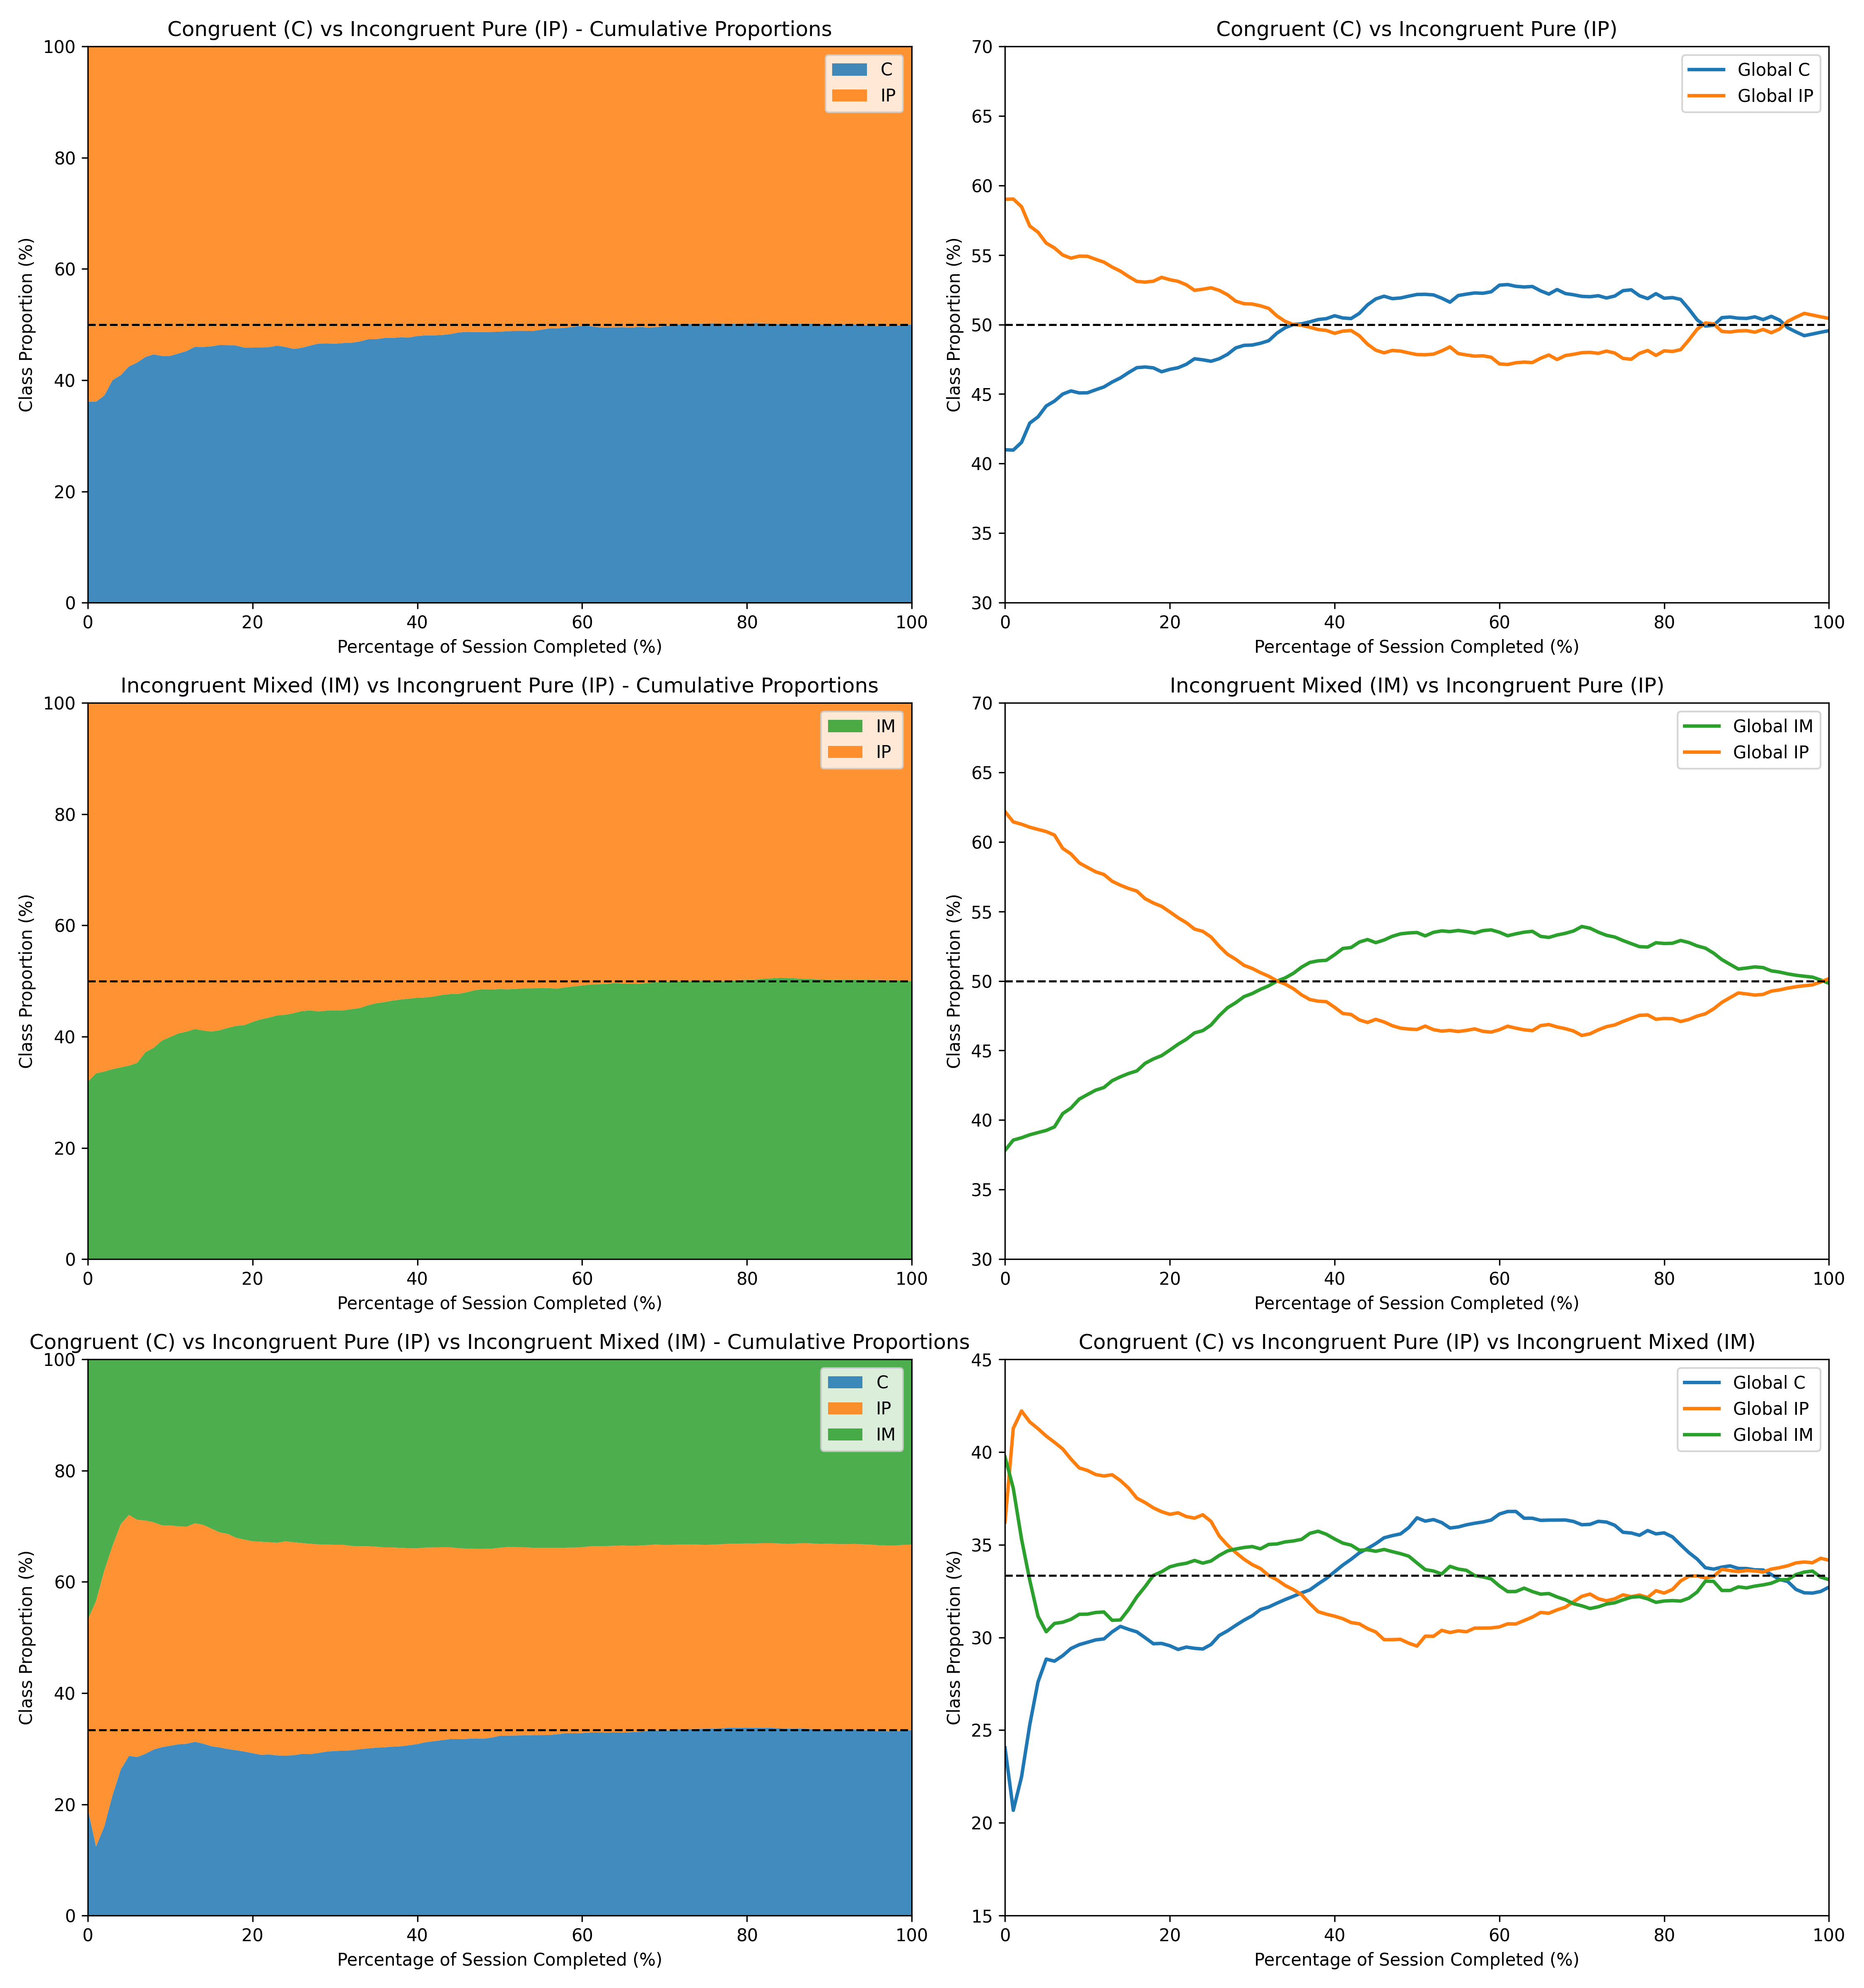
\includegraphics[width=0.6\textwidth]{images/class_drift.png}
    \caption{Class distribution and session drift diagnostics across the binocular-rivalry recordings.}
    \label{fig:class-drift}
\end{figure}

The temporal analysis of trial labels reveals non-stationarity in the proportion of C, IP, and IM trials across the session. This pattern is treated as a descriptive property of the dataset rather than as a new mechanistic result. It may reflect a mixture of perceptual adaptation, fatigue, attentional changes, and shifts in the participant's reporting criterion, but the present thesis does not try to separate these possibilities experimentally. The important consequence for the decoding analysis is simpler: trial order and session structure cannot be ignored.


The imbalance is not only a numerical inconvenience. It reflects the behavioral structure of the experiment: mixed percepts are common during incongruent stimulation, while pure incongruent reports are the minority class for the IM vs IP task. A naive classifier trained on unbalanced labels could therefore obtain misleading performance by exploiting prevalence, block structure, or subject-specific response tendencies. Balancing by subject is a conservative choice because it prevents a subject with many majority-class trials from dominating the pooled dataset, but it also discards data and makes variance larger. This trade-off is part of the interpretation of all reported accuracies.

The exploratory analysis identifies eye and color biases. In IP trials, left-eye coherent percepts are more frequent than right-eye coherent percepts, and red percepts are more frequent than green percepts. The red bias is interpreted in light of the luminance calibration described above: a slight overcorrection of the red--green balance could make red reports more likely even when the intended design was subjectively balanced. These biases are not modeled as separate predictors in the final decoding pipeline. Instead, the pipeline limits their influence indirectly through subject-wise balancing, grouped validation, and cautious interpretation of condition decoding.

These behavioral asymmetries also explain why the decoding results are interpreted against the background of eye dominance, color dominance, class imbalance, and temporal drift rather than as isolated model outputs.

\subsection{Subject Selection}
Session effects are difficult to remove perfectly after the fact, so they must be handled through validation design and interpretation. Randomly splitting trials can make adjacent or same-session trials appear in both training and validation folds, which risks inflating performance in EEG decoding \citep{white_k-fold_2023, del_pup_role_2025}. Grouped and chronological validation checks are therefore motivated by the exploratory structure of the dataset rather than added as an abstract machine-learning preference.

Subjects are selected using a minimum minority-class trial count and an effect-size criterion based on Cohen's $d$ \citep{lakens_calculating_2013}.\footnote{The selection score combines two practical requirements: enough minority-class trials to support balanced training, and a nonzero subject-level theta/alpha effect so that the selected cohort is informative for the EEG contrasts. The score is therefore a pragmatic analysis filter, not an independent claim that excluded participants lack rivalry-related EEG activity.} The main decoding cohorts contain 24 subjects for C vs IP and 29 subjects for IM vs IP. This selection is a compromise between statistical power and label quality. Including every subject would maximize sample size but may add subjects with too few minority-class trials for balanced training. Excluding too aggressively would make the cohort cleaner but less representative. Appendix~\ref{app:subject-selection} has more detail for each individual subject.

\chapter{Spatiotemporal Clustering}
\label{chap:clustering}

\section{From 1D Replication to 2D Clustering}
The original paper tests power changes in hypothesis-driven regions, especially fronto-medial theta around FCz and parieto-occipital alpha \citep{drew_conflict_2022, drew_binocular_2026}. These paper-derived ROIs are sensor groups and frequency bands defined in the original study, not regions selected from the present analyses. They provide a replication baseline before adding more flexible spatial statistics.

In this thesis, the 2D analysis aims to characterize the spatiotemporal extent of these reported effects: the EEG channels and time windows where each condition difference is most pronounced. To do this, the thesis applies cluster-based permutation testing in channel $\times$ time space, following non-parametric cluster statistics for electrophysiological data \citep{maris_nonparametric_2007}. This analysis is exploratory rather than confirmatory: it is used to describe broader, weaker, or spatially shifted effects, not to present a post-hoc search as an independent hypothesis test.

\section{Cluster Permutation}
The 2D method applies \textbf{cluster-based permutation testing} over channels and time. Each sample in the statistical map corresponds to one EEG channel and one time point. \textbf{Channel adjacency} is defined using a \textbf{Delaunay triangulation} of the 2D projected electrode coordinates, which determines which sensors are considered spatial neighbors, while temporal adjacency links consecutive time steps~\cite{maris_nonparametric_2007}. After applying a primary \textbf{cluster-forming threshold}, neighboring significant samples are grouped into spatiotemporal clusters, and each cluster $k$ is summarized by its \textbf{cluster mass} $M_k$:
\begin{equation}
    M_k = \sum_{(c,t) \in k} S(c,t),
\end{equation}
where $S(c,t)$ is the single-sample statistic (such as a $t$-value) at channel $c$ and time point $t$. The observed cluster masses are then compared with a permutation distribution of maximum cluster masses, producing family-wise corrected p-values \citep{maris_nonparametric_2007}. This makes the method well suited to EEG because it controls multiple comparisons without pretending that every channel-time sample is independent.

This procedure generates candidate clusters under several cluster-forming thresholds, together with uncorrected and corrected p-values. The selected cluster candidates are reported in Table~\ref{tab:selected-clusters}. They are therefore not automatic outputs accepted blindly from the test: the exported thresholds and windows are selected explicitly from the candidates, prioritising clusters that are interpretable and clear enough to describe as sensor-time patterns. This manual selection is part of the exploratory methodology; its implications for interpretation and circularity are discussed in Section~\ref{sec:cluster-roi-interpretation}.

The method also has an interpretive limit: cluster tests identify reliable regions of a sensor-time map, but they do not estimate exact neural onset times. A corrected cluster spanning 0.375--1.24 s should be read as evidence that the effect occupies that broad interval, not as proof that the process begins at exactly 375 ms. This distinction matters because the thesis later uses cluster windows to guide feature extraction and model interpretation. The cluster is evidence about a region of the data; it is not a precise event marker.

\begin{figure}[H]
    \centering
    \begin{minipage}{0.92\textwidth}
        \fbox{%
            \begin{minipage}{0.96\textwidth}
                \vspace{0.2cm}
                \textbf{\large Spatiotemporal Cluster Permutation Test} \\[0.3cm]
                The cluster-based permutation test \citep{maris_nonparametric_2007} controls the family-wise error rate (FWER) across the multi-sensor EEG time-series by grouping adjacent significant samples into clusters. The workflow is structured as follows:
                \begin{description}
                    \item[Step 1: Single-Sample Statistics] Compute the observed statistic (e.g., $t$-value) comparing experimental conditions at each individual channel-time sample $(c,t)$ to form a 2D map $S$.
                    \item[Step 2: Cluster Identification] Threshold the map $S$ using a primary cluster-forming threshold $\alpha_{cl}$ (typically $p < 0.05$). Group contiguous, suprathreshold samples into spatiotemporal clusters $C$ based on spatial adjacency (sensor neighborhood) and temporal contiguity.
                    \item[Step 3: Cluster Mass Calculation] For each identified cluster $c \in C$, calculate the overall cluster mass $M_c$ by summing all single-sample statistics within that cluster.
                    \item[Step 4: Permutation Distribution ($B$ runs)] Shuffle condition labels across trials to break the systematic experimental differences. Recompute the 2D statistical map for the permuted data, form clusters, and record the maximum cluster mass $M^{\max}_b$ from that run.
                    \item[Step 5: Significance Assessment] Compare each observed cluster mass $M_c$ against the empirical null distribution of maximum cluster masses. The FWER-corrected $p$-value is:
                          \begin{equation*}
                              p_c = \frac{1}{B} \sum_{b=1}^B \mathbb{I}(M^{\max}_b \ge M_c)
                          \end{equation*}
                \end{description}
                \vspace{0.2cm}
            \end{minipage}
        }
    \end{minipage}
    \caption{Workflow of the cluster-based permutation test for Monte Carlo multiple-comparison correction in spatiotemporal EEG datasets.}
    \label{fig:cluster-correction-pseudocode}
\end{figure}


To assess clustering variability, this analysis defines a subject-cohort divergence measure based on Jaccard overlap. For each selected cohort cluster, each subject's strongest signed spatiotemporal footprint is compared with the cohort footprint. The Jaccard similarity is
\begin{equation}
    J(A,B)=\frac{|A\cap B|}{|A\cup B|},
\end{equation}
where $A$ is the cohort cluster footprint and $B$ is the subject-level footprint. The reported variability measure is Jaccard divergence,
\begin{equation}
    D_J(A,B)=1-J(A,B).
\end{equation}
Values near 0 indicate that the subject footprint overlaps the cohort cluster strongly; values near 1 indicate that the subject's strongest effect lies in a different time-channel location. This is useful because it gives the cluster analysis a subject-level analogue of variability: instead of asking only whether a grand-average cluster exists, it asks whether individual subjects place their strongest effect in the same region.

\begin{figure}[H]
    \centering
    \resizebox{0.96\textwidth}{!}{%
        \begin{tikzpicture}[font=\small, node distance=8mm]
            \node[band, minimum width=34mm, minimum height=28mm] (mat) {};
            \foreach \x in {0,...,7} \foreach \y in {0,...,5} {
                    \pgfmathsetmacro{\inside}{(\x>=3)*(\x<=6)*(\y>=2)*(\y<=4)}
                    \pgfmathsetmacro{\shade}{\inside * (70 + 5*mod(\x+\y,3)) + (1 - \inside) * (12 + 8*mod(\x+\y,3))}
                    \fill[blue!\shade!white] ($(mat.south west)+(4mm+\x*3.2mm,4mm+\y*3.2mm)$) rectangle ++(2.8mm,2.8mm);
                }
            \draw[red!75!black, thick, rounded corners=2pt] ($(mat.south west)+(13mm,10mm)$) rectangle ++(12mm,10mm);
            \node[above=1mm of mat] {channel $\times$ time statistic};
            \node[feature, right=13mm of mat] (thr) {cluster-forming\\threshold};

            \node[band, right=10mm of thr, minimum width=28mm, minimum height=28mm] (topo) {};
            % Topoplot head outline
            \draw[black!55, thick] (topo.center) circle (1.1cm);
            % Nose
            \draw[black!55, thick] ($(topo.center)+(0,1.1)$) -- ($(topo.center)+(0.08,1.22)$) -- ($(topo.center)+(-0.08,1.22)$) -- cycle;
            % Ears
            \draw[black!55, thick] ($(topo.center)+(-1.1,0.1)$) .. controls ($(topo.center)+(-1.22,0.1)$) and ($(topo.center)+(-1.22,-0.1)$) .. ($(topo.center)+(-1.1,-0.1)$);
            \draw[black!55, thick] ($(topo.center)+(1.1,0.1)$) .. controls ($(topo.center)+(1.22,0.1)$) and ($(topo.center)+(1.22,-0.1)$) .. ($(topo.center)+(1.1,-0.1)$);

            % Electrode coordinates
            \coordinate (FP1) at ($(topo.center)+(-0.32, 0.72)$);
            \coordinate (FP2) at ($(topo.center)+(0.32, 0.72)$);
            \coordinate (F3) at ($(topo.center)+(-0.48, 0.38)$);
            \coordinate (FZ) at ($(topo.center)+(0.0, 0.42)$);
            \coordinate (F4) at ($(topo.center)+(0.48, 0.38)$);
            \coordinate (C3) at ($(topo.center)+(-0.62, 0.0)$);
            \coordinate (CZ) at ($(topo.center)+(0.0, 0.0)$);
            \coordinate (C4) at ($(topo.center)+(0.62, 0.0)$);
            \coordinate (P3) at ($(topo.center)+(-0.48, -0.38)$);
            \coordinate (PZ) at ($(topo.center)+(0.0, -0.42)$);
            \coordinate (P4) at ($(topo.center)+(0.48, -0.38)$);
            \coordinate (O1) at ($(topo.center)+(-0.28, -0.72)$);
            \coordinate (O2) at ($(topo.center)+(0.28, -0.72)$);

            % Adjacency lines
            \draw[teal!70!black, thick] (FP1) -- (F3) (FP2) -- (F4) (F3) -- (FZ) (F4) -- (FZ) (FZ) -- (CZ) (C3) -- (CZ) (C4) -- (CZ) (F3) -- (C3) (F4) -- (C4) (C3) -- (P3) (C4) -- (P4) (CZ) -- (PZ) (P3) -- (PZ) (P4) -- (PZ) (P3) -- (O1) (P4) -- (O2) (PZ) -- (O1) (PZ) -- (O2) (O1) -- (O2);

            % Electrode dots
            \foreach \pt in {FP1, FP2, F3, FZ, F4, C3, CZ, C4, P3, PZ, P4, O1, O2} {
                    \fill[teal!60!black] (\pt) circle (1.8pt);
                }

            \node[above=1mm of topo] {sensor adjacency};
            \node[statblock, right=12mm of topo] (mass) {cluster mass\\observed};
            \node[band, below=10mm of mass, minimum width=34mm, minimum height=18mm] (null) {};
            \foreach \x/\h in {0/4,1/6,2/5,3/9,4/7,5/6,6/11,7/5,8/8,9/6,10/7,11/5,12/9} {
                    \draw[purple!55, thick] ($(null.south west)+(2mm+\x*2.4mm,2mm)$) -- ++(0,\h mm);
                }
            \node[below=1mm of null] {max-mass permutation null};
            \node[statblock, left=12mm of null] (pval) {corrected\\$p$-value};
            \draw[arrow] (mat) -- (thr);
            \draw[arrow] (thr) -- (topo);
            \draw[arrow] (topo) -- (mass);
            \draw[arrow] (mass) -- (null);
            \draw[arrow] (null) -- (pval);
        \end{tikzpicture}
    }
    \caption{Cluster-based permutation pipeline for channel-by-time EEG statistics.}
    \label{fig:clustering-pipeline}
\end{figure}

\section{Cluster Results}
The results in this section are shown through a connected set of outputs. Figure~\ref{fig:replication-timepower-grid} provides the paper-derived ROI baseline, Figure~\ref{fig:data-driven-timepower-grid} shows the time courses after data-driven spatial selection, Table~\ref{tab:selected-clusters} lists the selected cluster candidates, and Figures~\ref{fig:cluster-topomap-progression}--\ref{fig:cvip-theta-cluster-heatmaps} make their spatial and temporal structure visible.

The exported C vs IP theta cluster includes Fz and FCz from approximately 1.17--1.24 s. It is spatially and temporally narrow, which matches the idea of a late fronto-medial conflict-related effect, but it is not the dominant sensor-time pattern in the dataset.

The C vs IP alpha cluster is broader and more stable. It covers parieto-occipital and central-posterior sensors from approximately 0.375--1.24 s. This is the strongest current clustering result. Within this chapter, the important point is that the clearest sensor-time pattern is posterior and distributed rather than concentrated in a single fronto-medial theta trace.

IM vs IP produces weaker and narrower clusters. The exported theta cluster includes Fz, FCz, and Cz from approximately 1.20--1.24 s, while the exported alpha cluster is limited to left posterior sensors from approximately 0.258--0.422 s. Scientifically, this is plausible because IM and IP are both incongruent conditions; the contrast is not simply conflict versus no conflict, but two different perceptual outcomes under conflict. A mixed report can also cover several subjective experiences, from local piecemeal mixtures to uncertain or unstable percepts. That heterogeneity can blur the group-level cluster.

The cluster results are easiest to read in three passes. First, the paper-derived ROIs, meaning the sensor groups and frequency bands defined from the source study rather than from the present dataset, ask whether the original theta/alpha story is visible in the same kind of summaries used by the source study. Second, the data-driven ROIs ask whether the strongest effects shift when the spatial region is selected from the current data. Third, global controls ask whether the effect depends completely on a narrow spatial prior.

\begin{figure}[H]
    \centering
    \panelimage{0.42\textwidth}{images/timecourse_v1_rep_c_vs_ip_theta.png}{C vs IP, fronto-medial theta.}
    \hfill
    \panelimage{0.42\textwidth}{images/timecourse_v1_rep_c_vs_ip_alpha.png}{C vs IP, parieto-occipital alpha.}
    \vspace{0.25cm}

    \panelimage{0.42\textwidth}{images/timecourse_v1_rep_im_vs_ip_theta.png}{IM vs IP, fronto-medial theta.}
    \hfill
    \panelimage{0.42\textwidth}{images/timecourse_v1_rep_im_vs_ip_alpha.png}{IM vs IP, parieto-occipital alpha.}
    \caption{Replication-style time-power plots in the paper-derived ROIs. These panels anchor the clustering chapter in the original theta/alpha hypotheses before introducing data-driven spatial selection.}
    \label{fig:replication-timepower-grid}
\end{figure}

Figure~\ref{fig:replication-timepower-grid} gives the replication baseline. The main visual result is not a strong theta separation at the ROI, but a clearer late alpha separation for C vs IP. This already hints that the most stable conflict-related structure in the current working dataset may be posterior and distributed rather than captured by a single fronto-medial theta trace.

\begin{figure}[H]
    \centering
    \panelimage{0.42\textwidth}{images/timecourse_v2_custom_c_vs_ip_theta.png}{C vs IP, data-driven theta ROI.}
    \hfill
    \panelimage{0.42\textwidth}{images/timecourse_v2_custom_c_vs_ip_alpha.png}{C vs IP, data-driven alpha ROI.}
    \vspace{0.25cm}

    \panelimage{0.42\textwidth}{images/timecourse_v2_custom_im_vs_ip_theta.png}{IM vs IP, data-driven theta ROI.}
    \hfill
    \panelimage{0.42\textwidth}{images/timecourse_v2_custom_im_vs_ip_alpha.png}{IM vs IP, data-driven alpha ROI.}
    \caption{Time-power plots after selecting data-driven spatial ROIs from the clustering analysis. The C vs IP alpha panel shows the most sustained cluster-consistent separation, whereas the IM vs IP panels are weaker and more sensitive to the selected window.}
    \label{fig:data-driven-timepower-grid}
\end{figure}

The data-driven ROI view in Figure~\ref{fig:data-driven-timepower-grid} strengthens that interpretation. C vs IP alpha remains the most sustained difference, while C vs IP theta becomes visible mainly as a late, narrower effect. The IM vs IP panels are informative mostly by contrast: they contain structured fluctuations, but they do not form the same broad and stable pattern.

The numerical cluster definitions in Table~\ref{tab:selected-clusters} provide the compact version of this story. They separate the strong C vs IP alpha cluster from the small C vs IP theta cluster and from the weaker IM vs IP clusters.

\begin{table}[H]
    \centering
    \caption{Selected exported spatiotemporal cluster candidates used for interpretation, including their cluster-forming threshold ($p_{\text{uncorrected}}$) and family-wise error corrected value ($p_{\text{corrected}}$).}
    \label{tab:selected-clusters}
    \begin{tabular}{llllll}
        \toprule
        Task     & Band  & Main channels / region         & Time window    & $p_{\text{uncorrected}}$ & $p_{\text{corrected}}$ \\
        \midrule
        C vs IP  & theta & Fz, FCz                        & 1.172--1.242 s & 0.01                     & 0.0240                 \\
        C vs IP  & alpha & broad parieto-occipital        & 0.375--1.242 s & 0.001                    & 0.0002                 \\
        IM vs IP & theta & Fz, FCz, Cz                    & 1.195--1.242 s & 0.05                     & 0.2461                 \\
        IM vs IP & alpha & TP7, CP5, CP3, CP1, P7, P5, P3 & 0.258--0.422 s & 0.05                     & 0.2713                 \\
        \bottomrule
    \end{tabular}
\end{table}

\begin{table}[H]
    \centering
    \small
    \caption{Subject-cohort clustering variability from the Jaccard divergence analysis. $D_J=1-J$; lower values are better.}
    \label{tab:jaccard-variability}
    \begin{tabular}{lllllll}
        \toprule
        Task     & Band  & ROI         & $n$ & Points & $D_J$             \\
        \midrule
        C vs IP  & theta & narrow      & 24  & 5      & $0.867 \pm 0.239$ \\
        C vs IP  & alpha & whole scalp & 24  & 581    & $0.687 \pm 0.117$ \\
        IM vs IP & theta & narrow      & 29  & 6      & $0.892 \pm 0.173$ \\
        IM vs IP & alpha & broad       & 29  & 34     & $0.946 \pm 0.111$ \\
        \bottomrule
    \end{tabular}
\end{table}

The Jaccard table is relevant because cluster significance and cluster stability are not the same claim. A cohort-level cluster can be statistically strong even if individual subjects vary substantially in the exact electrodes or time samples that carry the strongest effect. Conversely, a cluster with modest corrected evidence but low Jaccard divergence would be valuable because it would show subject-level consistency.

The divergences are high overall, so the stability result should be read cautiously. C vs IP alpha is the most stable cluster by this metric, with mean Jaccard divergence $D_J=0.687$ and the smallest standard deviation. This is still not low in an absolute sense: individual subject footprints overlap only partially with the cohort cluster. However, it is clearly less divergent than the other three cluster definitions, and it involves a much larger cohort footprint. This supports the interpretation that posterior alpha is the most reproducible clustering result in the thesis, but that even this effect is distributed and subject-variable rather than anatomically sharp.

The other clusters are much less stable. C vs IP theta has $D_J=0.867$ and contains only five channel-time points, so the subject-level footprints often shift away from the narrow cohort window. IM vs IP theta is similarly divergent ($D_J=0.892$), while IM vs IP alpha is the least stable result ($D_J=0.946$). This pattern strengthens the caution around IM vs IP. The mixed-versus-single-color contrast may contain some condition-related structure, but it is not expressed as a consistent shared sensor-time footprint across subjects. In practical terms, these Jaccard results argue against over-interpreting small IM vs IP clusters and in favor of presenting C vs IP alpha as the main clustering evidence.

The topographic grid in Figure~\ref{fig:cluster-topomap-progression} is included after the numerical tables because its job is explanatory rather than statistical. It shows what the selected clusters look like on the scalp at representative times, making the broad posterior alpha pattern and the narrow frontal theta pattern visually inspectable.

\begin{figure}[H]
    \centering
    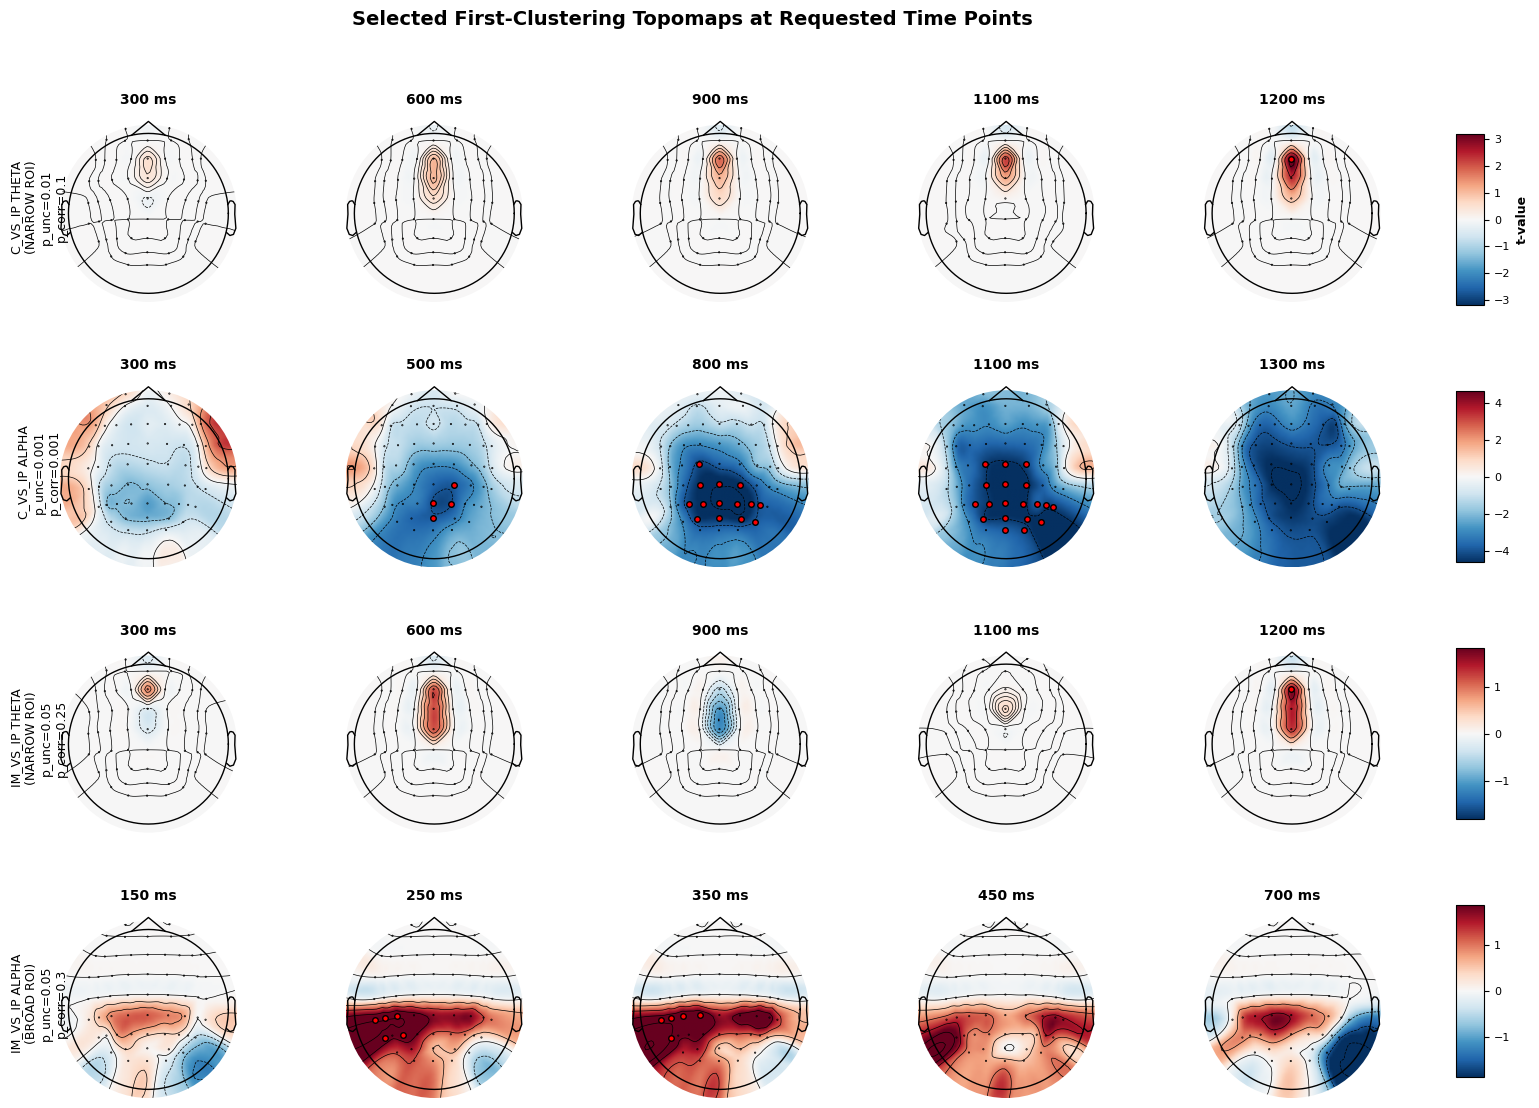
\includegraphics[width=0.9\textwidth]{images/clustering_topomaps.png}
    \caption{Selected cluster topomaps at representative time points. The grid complements the numerical cluster table by showing how the selected patterns extend across sensors and time for theta and alpha contrasts.}
    \label{fig:cluster-topomap-progression}
\end{figure}

At first glance, the clusters for the alpha bands are wider---they include more electrode channels and are detected throughout different time points. The alpha clusters also appear sooner, while the theta clusters show up near the end.

The latency maps then compress this same information into a timing summary.

\begin{figure}[H]
    \centering
    \panelimage{0.42\textwidth}{images/onset_map_theta.png}{Theta onset latency map.}
    \hfill
    \panelimage{0.42\textwidth}{images/onset_map_alpha.png}{Alpha onset latency map.}
    \caption{Latency maps for the first time to significant decoding in the C vs IP task in theta and alpha. They are interpreted as coarse spatial timing summaries, not as exact neural onset estimates.}
    \label{fig:onset-latency-maps}
\end{figure}


The C vs IP theta cluster was chosen as a representative example of the results of the clustering. Since the unrestricted candidate clusters were very far from significance ($p_\text{corrected}>0.3$), the search was restricted to only 3 electrodes. Figure~\ref{fig:cvip-theta-cluster-heatmaps} shows both the surrounding unmasked trend and the final masked selection, with a final $p_\text{corrected}<0.1$, which is not statistically significant, but it's much closer than before, and is much more likely to be able to separate the two classes.

\begin{figure}[H]
    \centering
    \panelimage{0.48\textwidth}{images/cluster_c_vs_i_theta_narrow.png}{Unmasked narrow theta cluster.}
    \hfill
    \panelimage{0.48\textwidth}{images/final_masked_heatmap_c_vs_ip_theta_narrow.png}{Final masked theta selection.}
    \caption{C vs IP theta cluster heatmaps. The unmasked map shows the broader late positive trend across Fz/FCz/Cz, while the masked map isolates the final selected cluster used for interpretation.}
    \label{fig:cvip-theta-cluster-heatmaps}
\end{figure}

The ROIs from the original paper and the 2D clusters are therefore treated as complementary summaries. The former keep the analysis anchored in the source study, while the latter show whether the present dataset contains broader or shifted sensor-time effects. Their different roles, and the circularity risk introduced by data-driven cluster selection, are discussed in the next section.

\section{Interpretation of cluster-based and ROI analyses}
\label{sec:cluster-roi-interpretation}

The sensor-time cluster analysis was used to assess whether the differences between congruent and incongruent images extend beyond the regions and time windows reported in the original study. This analysis follows the logic of cluster-based permutation testing, in which neighboring sensors and time points are grouped to address the multiple-comparisons problem in EEG data.

The ROIs derived from the previous study and the data-driven clusters play different roles. The paper-derived ROIs are hypothesis-driven: they test whether the present dataset replicates the previously reported frontal theta and occipital alpha effects. In contrast, the sensor-time clusters are exploratory: they indicate whether the present data show broader, weaker, or spatially shifted effects.

A circularity problem would arise if the same data were used first to define a cluster and then to make a confirmatory claim about effect size or decoding performance within that same cluster \citep{kriegeskorte_circular_2009}. In that case, the estimate could be biased because the region was selected precisely because it showed a difference in the current dataset. For this reason, cluster-defined regions are used here mainly for interpretation and visualization. Confirmatory conclusions rely primarily on analyses defined independently of the current data, such as the paper-derived ROIs, and on decoding performance evaluated on held-out data.

Therefore, the cluster results should be interpreted as complementary evidence rather than as the sole basis for the main conclusion. Consistent effects across the original ROIs, sensor-time clusters, time-frequency representations, topographies, and decoding analyses would support the interpretation that congruent and incongruent images modulate frontal theta and occipital alpha activity in the present dataset.

\chapter{Decoding Methods}
\label{chap:methods}

\section{Overview}
The decoding analyses test whether single-trial EEG activity contains information about the perceptual condition. Two binary contrasts are considered. C vs IP compares compatible trials with incompatible trials that still lead to a single-color report. This is the cleaner conflict-related contrast because both classes involve the same type of report, while the physical stimulus differs in the presence of interocular conflict. IM vs IP compares mixed and single-color reports within incompatible stimulation. This contrast is more exploratory because the physical stimulation is incompatible in both classes and the label depends more directly on the subjective perceptual report.

The models are organized as a hierarchy of increasing flexibility. First, simple hypothesis-driven models test whether fronto-medial theta or parieto-occipital alpha features are sufficient for classification. Second, covariance-based Riemannian decoding tests whether distributed multichannel structure carries additional discriminative information. Third, compact and pretrained deep-learning models are evaluated as exploratory baselines. This organization avoids treating model complexity as an end in itself: the main question is whether richer EEG representations improve decoding beyond interpretable EEG features.

\section{Cross-Validation and Leakage Control}
All decoding analyses were evaluated using a leakage-aware validation strategy. This is essential for EEG because trials recorded close in time may share slow drifts, artifacts, fatigue effects, adaptation, or response biases. If consecutive trials are split randomly between training and validation folds, the classifier may exploit temporal dependencies in the recording rather than condition-related neural information, and may overestimate the true decoding capacity \citep{white_k-fold_2023, del_pup_role_2025}.

To reduce this risk, the analyses used \textbf{Stratified Group K-fold cross-validation}. Stratification preserves class proportions across folds, while grouping prevents temporally related trials from being split arbitrarily between training and validation sets.\footnote{In this thesis, groups correspond to temporally local trial blocks within each participant's recording rather than to individual samples. The exact grouping unit is chosen in the executable pipeline so that adjacent or near-adjacent trials are kept together during validation.} Thus, stratification addresses class imbalance, whereas grouping addresses temporal dependence and potential leakage across consecutive trials. This is not a hypothetical concern in the present dataset: a mean Pearson temporal autocorrelation of 0.56 was estimated between nearby trial representations, indicating strong temporal dependence across the session.

All preprocessing steps that estimate parameters from the data were performed within the training folds and then applied to the corresponding validation fold. This includes feature scaling, covariance estimation, dimensionality reduction when used, and any model-specific transformation learned from the data. This fold-contained procedure prevents information from the validation fold from influencing the representation learned during training.

Balanced accuracy was used as the main performance metric because the number of trials per class can differ across subjects and conditions. In addition, permutation tests were used to estimate the null distribution of the complete decoding pipeline. This allows the observed decoding performance to be compared against the performance expected when labels are randomly shuffled while preserving the same validation structure.

\begin{figure}[H]
    \centering
    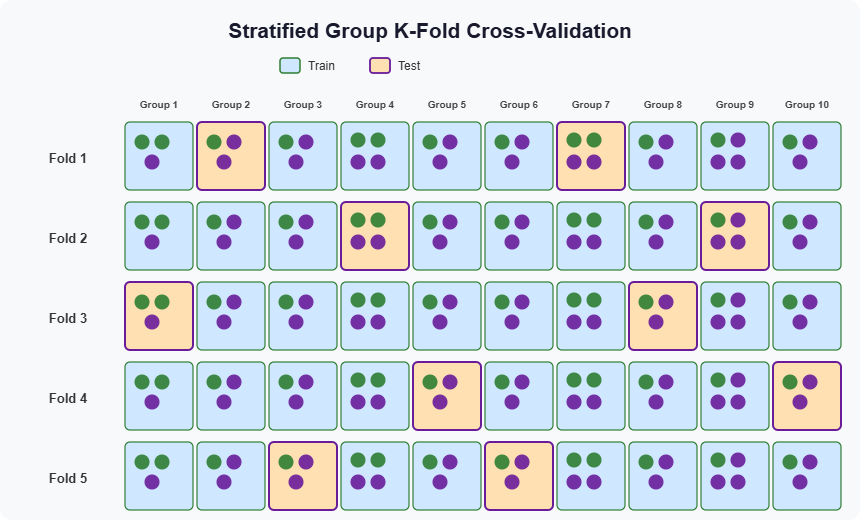
\includegraphics[width=0.82\textwidth]{images/stratified_group_k-fold_cv.png}
    \caption{Stratified Group K-fold cross-validation. Stratification preserves class proportions across folds, whereas grouping reduces leakage between consecutive EEG trials.}
    \label{fig:stratified-group-cv}
\end{figure}

\section{Classical and Hypothesis-Driven Decoders}
The first set of models used simple, hypothesis-driven EEG features. These models were motivated by the main effects examined in the previous analyses, especially fronto-medial theta and parieto-occipital alpha modulations. For each trial, the targeted logistic-regression pipeline filters one channel in one band, extracts the mean Hilbert envelope, scales features inside the training fold, and fits L2-regularized logistic regression. FCz-theta and Oz-alpha are the main theory-driven baselines.

These models serve as interpretable reference points. If a single fronto-medial theta or parieto-occipital alpha feature achieves above-chance decoding, the result is easy to relate to the time-frequency analyses. If these models fail, the failure is also informative because it suggests that the discriminative information is not captured by a single channel-band summary.

Additional classical classifiers were also evaluated on the same feature families. This classifier sweep separates two questions that are easy to conflate: whether the selected representation contains discriminative information, and whether a more flexible classifier can exploit that information better. The purpose of this sweep was not to exhaustively optimise performance, but to check whether the conclusions depended strongly on the choice of classifier.

\section{Riemannian Covariance Decoding}
Riemannian covariance decoding was used as the main multichannel classical approach. Unlike single-feature models, covariance-based methods represent each trial through the relationships between EEG channels. This is appropriate for scalp EEG because condition-related information may be spatially distributed and mixed across sensors by volume conduction.

For each trial, the covariance matrix is
\begin{equation}
    C^{(i)} = \frac{1}{T-1}(X^{(i)}-\bar{X}^{(i)})(X^{(i)}-\bar{X}^{(i)})^\top.
\end{equation}
Here, $X^{(i)}$ is the multichannel EEG signal for trial $i$, and $T$ is the number of time samples. The pipeline uses OAS shrinkage, tangent-space projection, and shrinkage LDA. The tangent-space projection allows covariance matrices to be analyzed with standard linear methods while preserving the geometry of the covariance representation.

This model occupies an important position in the decoding hierarchy. It remains relatively simple and low-capacity, but it can capture distributed spatial structure that is invisible to single-electrode power summaries. Therefore, it provides a strong classical benchmark against which more flexible models can be compared.

\begin{figure}[H]
    \centering
    \resizebox{0.95\textwidth}{!}{%
        \begin{tikzpicture}[
                font=\small,
                >=Latex,
                node distance=1.6cm,
                box/.style={draw, rounded corners, align=center, minimum height=1.0cm, minimum width=2.5cm},
                smallbox/.style={draw, rounded corners, align=center, minimum height=0.9cm, minimum width=2.3cm},
                arrow/.style={->, thick}
            ]
            \node[box] (epochs) {Balanced EEG epochs\\$N \times C \times T$};

            \node[smallbox, above right=1.0cm and 2.0cm of epochs] (features) {Hypothesis-driven\\band-power features\\theta / alpha};
            \node[smallbox, below right=1.0cm and 2.0cm of epochs] (cov) {regularized covariance\\matrices\\$C \times C$};

            \node[smallbox, right=2.3cm of features] (lr) {Logistic regression\\or classical ML};
            \node[smallbox, right=2.3cm of cov] (lda) {Tangent space\\+ LDA};

            \node[box, right=2.4cm of epochs] (eval) {Fold-contained\\evaluation\\balanced accuracy\\+ permutations};

            \draw[arrow] (epochs.east) -- ++(0.7,0) |- (features.west);
            \draw[arrow] (epochs.east) -- ++(0.7,0) |- (cov.west);
            \draw[arrow] (features.east) -- (lr.west);
            \draw[arrow] (cov.east) -- (lda.west);
            \draw[arrow] (lr.east) -- ++(0.7,0) |- (eval.north);
            \draw[arrow] (lda.east) -- ++(0.7,0) |- (eval.south);
        \end{tikzpicture}
    }
    \caption{Classical decoding pipelines. Hypothesis-driven band-power features and Riemannian covariance representations are treated as alternative feature spaces, not as sequential steps. All transformations are estimated within the training folds and evaluated on held-out data.}
    \label{fig:classical-riemannian-pipeline}
\end{figure}

\section{Cluster-Restricted Decoding}
Cluster-restricted classifiers were used to test whether sensor-time regions identified in the statistical analyses also contained discriminative information. These models used compact theta/alpha summaries extracted from selected cluster windows and classified them with a support vector classifier or related classical models. They act as a bridge between simple linear baselines and deep models: more flexible than logistic regression, but still interpretable through the cluster features.

These analyses should be interpreted as exploratory unless the cluster selection is performed independently of the decoding evaluation. If the same dataset is used first to identify a cluster and then to estimate decoding performance within that cluster, the performance estimate may be optimistic because the feature space has already been selected using condition-related information. A confirmatory cluster-restricted analysis would require either clusters defined from a previous study or cluster selection performed separately within each training fold.

Together, these classical approaches define a useful ladder of assumptions. Logistic regression asks whether a single theory-driven scalar is enough. Riemannian covariance asks whether distributed spatial relationships carry the signal. Cluster-restricted SVC asks whether selected sensor-time regions can support a slightly more flexible decision boundary. This ladder is important because it prevents the thesis from jumping directly from a hand-designed baseline to deep learning. It shows how much is gained by changing the representation before changing the model family.

\section{Deep-Learning Baselines}
Deep-learning models were included as exploratory baselines to test whether learned spatiotemporal representations improved decoding beyond the classical approaches. Because the dataset is limited and the decoding contrasts are subtle, these models are not treated as the primary evidence of the thesis. Their role is to compare modern EEG architectures under the same validation constraints and to test whether additional model flexibility changes the interpretation established by the classical pipelines.

\subsection{EEGNet}
The main compact neural-network baseline was EEGNet, an architecture designed specifically for EEG classification \citep{lawhern_eegnet_2018}. EEGNet combines temporal convolutions, depthwise spatial filtering, separable convolutions, pooling, dropout, and a small classification head. Conceptually, this resembles a learned version of temporal filtering followed by spatial projection, making it a useful lightweight EEG-specific baseline.

The original motivation of EEGNet was not binocular rivalry, but EEG-based brain-computer interfaces. \citeauthor{lawhern_eegnet_2018} designed it as a compact model that could generalize across several standard BCI paradigms, including P300 visual evoked potentials, error-related negativity, movement-related cortical potentials, and sensorimotor rhythms \citep{lawhern_eegnet_2018}. This makes it a useful baseline here: it is small enough for limited EEG data, but general enough that it is not tied to one specific oscillatory signature. In the agnostic 60-channel, 0--1.5 s configuration used in the notebooks, the implemented model receives 192 time samples after resampling and has 2,258 parameters, all of which are trained from scratch. This means the trainable proportion is 100\%; there is no frozen pretrained component. Of these parameters, 194 belong to the final classifier and the rest belong to the temporal, depthwise spatial, separable convolution, and normalization layers. The cluster-restricted EEGNet variants are similarly small, with parameter counts changing only because the number of selected channels and time samples changes.

The project tests two EEGNet variants. The agnostic variant receives all 60 channels and broadband input, asking whether the network can discover useful spatial and temporal filters without being told where the theta or alpha effects should be. The cluster-restricted variant receives a more constrained input based on the data-driven clusters, asking whether statistical prior information helps the network focus on biologically plausible regions. The comparison is informative even when performance is modest: it tests whether constraining the input around interpretable EEG regions helps learning, or whether the selected clusters are too narrow for the decoding task.

\begin{figure}[H]
    \centering
    \resizebox{0.92\textwidth}{!}{%
        \begin{tikzpicture}[font=\scriptsize, >=Latex]
            \drawnetworkblock{eeg_in}{0.0}{0.0}{0.25}{1.6}{1.0}{blue!20}{\tiny EEG}{Input\\1 $\times$ 60 $\times$ 192}
            \draw[blue!65!black, very thin] (0.02, 0.3) -- (0.05, 0.34) -- (0.08, 0.24) -- (0.11, 0.32) -- (0.14, 0.22) -- (0.17, 0.33) -- (0.20, 0.28);
            \draw[blue!65!black, very thin] (0.02, 1.3) -- (0.05, 1.34) -- (0.08, 1.24) -- (0.11, 1.32) -- (0.14, 1.22) -- (0.17, 1.33) -- (0.20, 1.28);
            \drawnetworkblock{eeg_temp}{1.6}{0.0}{0.5}{1.6}{1.0}{red!20}{\tiny Temp}{Temporal Conv\\8 $\times$ 60 $\times$ 192}
            \fill[red!80, opacity=0.5] (0.05, 0.4) rectangle (0.2, 1.2);
            \draw[red!60, dashed, very thin] (0.2, 0.4) -- (eeg_temp-frontbottomleft);
            \draw[red!60, dashed, very thin] (0.2, 1.2) -- (eeg_temp-fronttopleft);
            \drawnetworkblock{eeg_spatial}{3.4}{0.6}{0.8}{0.4}{1.0}{red!30}{\tiny Spat}{Depthwise Spatial\\16 $\times$ 1 $\times$ 192}
            \fill[red!80, opacity=0.5] (1.7, 0.0) rectangle (2.0, 1.6);
            \draw[red!60, dashed, very thin] (2.0, 0.0) -- (eeg_spatial-frontbottomleft);
            \draw[red!60, dashed, very thin] (2.0, 1.6) -- (eeg_spatial-fronttopleft);
            \drawnetworkblock{eeg_pool1}{5.2}{0.6}{0.6}{0.4}{0.4}{cyan!25}{\tiny Pool}{AvgPool\\16 $\times$ 1 $\times$ 48}
            \drawnetworkblock{eeg_sep}{6.8}{0.6}{0.6}{0.4}{0.4}{red!40}{\tiny Sep}{Separable Conv\\16 $\times$ 1 $\times$ 48}
            \drawnetworkblock{eeg_pool2}{8.4}{0.6}{0.6}{0.4}{0.15}{cyan!35}{\tiny Pool}{AvgPool\\16 $\times$ 1 $\times$ 6}
            \drawnetworkblock{eeg_out}{10.0}{0.3}{0.2}{1.0}{0.2}{purple!20}{\tiny FC}{Linear\\2 classes}
            \draw[arrow] (eeg_in-rightcenter) -- (eeg_temp-leftcenter);
            \draw[arrow] (eeg_temp-rightcenter) -- (eeg_spatial-leftcenter);
            \draw[arrow] (eeg_spatial-rightcenter) -- (eeg_pool1-leftcenter);
            \draw[arrow] (eeg_pool1-rightcenter) -- (eeg_sep-leftcenter);
            \draw[arrow] (eeg_sep-rightcenter) -- (eeg_pool2-leftcenter);
            \draw[arrow] (eeg_pool2-rightcenter) -- (eeg_out-leftcenter);
        \end{tikzpicture}
    }
    \caption{EEGNet architecture used as the compact EEG-specific convolutional baseline.}
    \label{fig:eegnet-architecture}
\end{figure}

\subsection{Spatio-Temporal Graph Neural Network}
A spatio-temporal graph neural network was also evaluated to test whether the scalp montage structure helps decoding. The model represents EEG sensors as nodes in an electrode graph. Edges encode spatial adjacency, so information can propagate between nearby electrodes according to the montage rather than according to an arbitrary channel ordering. This is attractive for EEG because the sensor layout is neither a regular image grid nor a meaningful one-dimensional sequence.

Unlike ST-EEGFormer and LaBraM, this model is not used as a pretrained foundation model. It is a task-specific architecture trained from scratch, motivated by the broader family of graph neural networks for EEG classification \citep{klepl_graph_2024}. The local implementation uses spectral graph convolution through Chebyshev filters, followed by a temporal convolutional stage, global node pooling, and a linear classifier. For the 60-node electrode graph with theta and alpha node features used here, the model has 23,010 parameters and all 23,010 are trainable. The trainable proportion is therefore 100\%; the graph convolution, temporal convolution, batch normalization, pooling pathway, and classifier are all adapted to the binocular-rivalry data rather than inherited from another corpus.

In this thesis, the graph model is used as an intermediate point between compact convolutional models and larger transformer-style models. Its spatial part is intended to capture local sensor relationships, while its temporal part summarizes activity over the trial window. The expectation is not that it will automatically beat Riemannian covariance; rather, it tests whether learnable spatial message passing can recover useful conflict-related patterns from limited data.

\begin{figure}[H]
    \centering
    \resizebox{0.82\textwidth}{!}{%
        \begin{tikzpicture}[font=\scriptsize, >=Latex]
            \drawnetworkblock{gnn_in}{0.0}{0.0}{1.2}{1.6}{0.4}{blue!15}{\scriptsize Graph}{Electrode Graph\\60 nodes}
            \fill[teal] (0.2, 0.4) circle (1.2pt) (0.4, 1.2) circle (1.2pt) (1.0, 0.5) circle (1.2pt) (0.9, 1.3) circle (1.2pt) (0.6, 0.7) circle (1.2pt);
            \draw[black!55, very thin] (0.2, 0.4) -- (0.6, 0.7) -- (1.0, 0.5) -- (0.9, 1.3) -- (0.4, 1.2) -- (0.2, 0.4) (0.6, 0.7) -- (0.4, 1.2) (0.6, 0.7) -- (0.9, 1.3);
            \drawnetworkblock{gnn_cheb}{2.2}{0.0}{1.2}{1.6}{0.6}{red!25}{\tiny Cheb}{Graph Conv\\32 hidden}
            \drawnetworkblock{gnn_temp}{4.4}{0.0}{1.2}{1.6}{0.6}{red!35}{\tiny Temp}{Temporal Conv\\64 hidden}
            \drawnetworkblock{gnn_pool}{6.6}{0.6}{1.2}{0.4}{0.6}{cyan!25}{\tiny Pool}{Global Mean\\Node Pooling}
            \drawnetworkblock{gnn_out}{8.8}{0.3}{0.2}{1.0}{0.2}{purple!20}{\tiny FC}{Linear\\2 classes}
            \draw[arrow] (gnn_in-rightcenter) -- (gnn_cheb-leftcenter);
            \draw[arrow] (gnn_cheb-rightcenter) -- (gnn_temp-leftcenter);
            \draw[arrow] (gnn_temp-rightcenter) -- (gnn_pool-leftcenter);
            \draw[arrow] (gnn_pool-rightcenter) -- (gnn_out-leftcenter);
        \end{tikzpicture}
    }
    \caption{Spatio-temporal graph neural network architecture based on electrode adjacency and temporal convolution.}
    \label{fig:stgnn-architecture}
\end{figure}

\subsection{ST-EEGFormer}
ST-EEGFormer is included to test a transformer-style approach to EEG. The model converts the EEG epoch into tokens, combines temporal and spatial positional information, processes the sequence through attention blocks, and feeds the resulting representation to a classification head. In principle, attention can model long-range dependencies between channels and time segments more flexibly than a small convolutional network. This could be useful if the perceptual-conflict signature is distributed across both space and time.

The model is especially relevant because it was introduced as a transformer-style EEG foundation-model baseline rather than as a task-specific binocular-rivalry decoder. The cited ST-EEGFormer work pretrains a ViT-like EEG encoder with masked autoencoding on more than eight million EEG segments, then evaluates whether the learned representation transfers to diverse BCI tasks \citep{yang_are_2025}. This pretraining objective is conceptually attractive for this thesis because it teaches the model to reconstruct missing EEG structure without using the downstream labels. However, the pretraining data and objectives are still far from onset binocular rivalry, so transfer cannot be assumed.

The practical constraints are substantial. The implementation resamples from 500 Hz to 128 Hz and aligns the data to the 142-channel montage expected by the ST-EEGFormer checkpoint, so the input is not identical to the classical or EEGNet pipelines. In the local 142-channel adaptation, the MAE/Vision-Transformer backbone plus binary classifier has 25,829,250 parameters, of which 534,018 are trainable, corresponding to 2.1\% of the model. The fine-tuned layers are deliberately restricted: rank-8 LoRA adapters with $\alpha=16$ and dropout 0.05 are injected into attention and MLP linear layers, the patch embedding remains trainable, and a task-specific linear classifier is trained on top of the frozen backbone representation \citep{hu_lora_2022}. The remaining pretrained transformer parameters are frozen. The interpretation of ST-EEGFormer results must therefore be pipeline-aware: a weak result may reflect architecture limitations, but it may also reflect resampling, channel mapping, token format, insufficient fine-tuning data, or mismatch between pretrained assumptions and the binocular-rivalry task.

\begin{figure}[H]
    \centering
    \resizebox{0.88\textwidth}{!}{%
        \begin{tikzpicture}[font=\scriptsize, >=Latex]
            \draw[draw=black!40, fill=blue!5, rounded corners=1.5pt] (0.0,0.0) rectangle (0.8,1.2);
            \foreach \y in {0.2,0.4,0.6,0.8,1.0} {
                    \draw[blue!60, opacity=0.8, thin] (0.05, \y) -- (0.1, \y+0.04) -- (0.15, \y-0.05) -- (0.2, \y+0.03) -- (0.25, \y-0.03) -- (0.3, \y+0.05) -- (0.35, \y-0.04) -- (0.4, \y+0.06) -- (0.45, \y-0.05) -- (0.5, \y+0.03) -- (0.55, \y-0.04) -- (0.6, \y+0.04) -- (0.65, \y-0.03) -- (0.7, \y+0.05) -- (0.75, \y);
                }
            \draw[black!50, dotted] (0.2, 0) -- (0.2, 1.2);
            \draw[black!50, dotted] (0.4, 0) -- (0.4, 1.2);
            \draw[black!50, dotted] (0.6, 0) -- (0.6, 1.2);
            \node[anchor=north, align=center, font=\tiny] at (0.4,-0.05) {Input EEG\\142 $\times$ 192};
            \node[draw=black!70, fill=red!10, rounded corners=2pt, minimum height=1.2cm, text width=1.1cm, align=center] (patch) at (2.0,0.6) {Patch\\Embed};
            \foreach \y in {0.1, 0.3, 0.5, 0.7, 0.9, 1.1} {\draw[draw=teal!70!black, fill=teal!15] (3.1, \y-0.07) rectangle (3.3, \y+0.07);}
            \node[anchor=north, font=\tiny] at (3.2, -0.05) {Tokens};
            \node[draw, circle, inner sep=1.5pt, fill=yellow!15, thick] (add) at (4.0, 0.6) {\tiny $+$};
            \node[draw=black!50, fill=yellow!5, rounded corners=1pt, font=\tiny, align=center, inner sep=2pt] (tpe) at (4.0, 1.4) {Temp PE};
            \node[draw=black!50, fill=yellow!5, rounded corners=1pt, font=\tiny, align=center, inner sep=2pt] (spe) at (4.0, -0.2) {Spat PE};
            \node[draw=black!70, fill=green!15, rounded corners=2pt, minimum height=1.6cm, text width=1.8cm, align=center] (encoder) at (5.8,0.6) {Transformer\\Encoder\\8 blocks};
            \node[draw=black!70, fill=cyan!10, rounded corners=2pt, minimum height=1.2cm, text width=1.1cm, align=center] (avg) at (7.9,0.6) {Token\\Average};
            \node[draw=black!70, fill=purple!10, rounded corners=2pt, minimum height=1.2cm, text width=1.1cm, align=center] (clf) at (9.6,0.6) {Linear\\Head};
            \node[align=left, font=\tiny] (out_tf) at (11.1,0.6) {2 classes};
            \draw[arrow] (0.8,0.6) -- (patch.west);
            \draw[arrow] (patch.east) -- (3.05, 0.6);
            \draw[arrow] (3.35, 0.6) -- (add.west);
            \draw[thinarr] (tpe.south) -- (add.north);
            \draw[thinarr] (spe.north) -- (add.south);
            \draw[arrow] (add.east) -- (encoder.west);
            \draw[arrow] (encoder.east) -- (avg.west);
            \draw[arrow] (avg.east) -- (clf.west);
            \draw[arrow] (clf.east) -- (out_tf.west);
        \end{tikzpicture}
    }
    \caption{ST-EEGFormer adaptation with channel-aligned, resampled EEG input, patch embedding, temporal/spatial positional encodings, transformer encoder blocks, LoRA fine-tuning, and a linear head.}
    \label{fig:steegformer-architecture}
\end{figure}

\subsection{LaBraM}
Large Brain Model, or LaBraM, is a patch-based pretrained EEG foundation model adapted here with LoRA-style fine-tuning. Its appeal is straightforward: a model pretrained on large EEG corpora might learn reusable temporal and spatial structure that a small thesis dataset cannot provide on its own. In principle, this could help when the downstream labels are subtle and the number of task-specific trials is limited.

LaBraM was originally proposed as a large EEG model for generic BCI representation learning, not as a model for visual rivalry specifically. Its pretraining strategy addresses a practical EEG problem: datasets differ in channel layouts, trial lengths, tasks, and signal quality. LaBraM therefore segments EEG into channel-level patches, uses a vector-quantized neural spectrum tokenizer to convert continuous EEG patches into discrete neural codes, and trains transformer blocks to predict masked neural codes. The reported pretraining corpus contains approximately 2,500 hours of EEG from around 20 datasets, with downstream evaluations including abnormal detection, event type classification, emotion recognition, and gait prediction \citep{jiang_large_2024}. This makes LaBraM the most explicitly large-scale pretrained model in the thesis, but also the model with the greatest possible domain gap from the present onset-rivalry task.

I used Braindecode's pretrained \texttt{InterpolatedLaBraM} wrapper with 60 input channels, 200 time samples, patch size 200, a neural tokenizer, 12 transformer blocks, embedding dimension 200, and 10 attention heads. The saved fold weights used for the final check show rank-8 LoRA adapters with $\alpha=16$ and dropout 0.2 in the attention and MLP linear layers, with the temporal tokenizer and binary final layer also trainable \citep{hu_lora_2022}. This corresponds to 308,178 trainable parameters in the saved fold, about 5.3\% of the approximately 5.8M-parameter adapted model; the pretrained transformer body remains frozen. The current results do not show a clear advantage over classical methods, and that negative result is useful. Foundation models are not magic feature extractors; they depend on checkpoint compatibility, channel layout, sampling rate, patch construction, pretraining domain, and the fine-tuning objective. A model pretrained on one family of EEG tasks may not transfer cleanly to onset binocular rivalry. LaBraM is therefore treated as an exploratory model in this thesis. Its role is to test whether a modern pretrained EEG representation helps under realistic constraints, not to draw a general conclusion about the value of EEG foundation models.

\begin{figure}[H]
    \centering
    \resizebox{0.82\textwidth}{!}{%
        \begin{tikzpicture}[font=\scriptsize, >=Latex]
            \draw[draw=black!40, fill=blue!5, rounded corners=1.5pt] (0.0,0.0) rectangle (0.8,1.2);
            \foreach \y in {0.2,0.4,0.6,0.8,1.0} {
                    \draw[blue!60, opacity=0.8, thin] (0.05, \y) -- (0.1, \y+0.04) -- (0.15, \y-0.05) -- (0.2, \y+0.03) -- (0.25, \y-0.03) -- (0.3, \y+0.05) -- (0.35, \y-0.04) -- (0.4, \y+0.06) -- (0.45, \y-0.05) -- (0.5, \y+0.03) -- (0.55, \y-0.04) -- (0.6, \y+0.04) -- (0.65, \y-0.03) -- (0.7, \y+0.05) -- (0.75, \y);
                }
            \draw[black!50, dotted] (0.2, 0) -- (0.2, 1.2);
            \draw[black!50, dotted] (0.4, 0) -- (0.4, 1.2);
            \draw[black!50, dotted] (0.6, 0) -- (0.6, 1.2);
            \node[anchor=north, align=center, font=\tiny] at (0.4,-0.05) {Input\\patches};
            \node[draw=black!70, fill=red!10, rounded corners=2pt, minimum height=1.2cm, text width=1.2cm, align=center] (tokenizer) at (2.0,0.6) {Neural\\Tokenizer};
            \node[draw=black!70, fill=gray!25, rounded corners=2pt, minimum height=1.2cm, text width=1.8cm, align=center] (pretrained) at (4.6,1.4) {Pretrained\\Transformer\\frozen blocks};
            \node[draw=black!70, fill=orange!15, rounded corners=2pt, minimum height=1.2cm, text width=1.8cm, align=center] (lora) at (4.6,-0.2) {LoRA\\Adapters\\trainable};
            \node[draw, circle, inner sep=1.5pt, fill=yellow!15, thick] (merge) at (7.0, 0.6) {\tiny $+$};
            \node[draw=black!70, fill=purple!10, rounded corners=2pt, minimum height=1.2cm, text width=1.1cm, align=center] (clf_l) at (8.5,0.6) {Linear\\Head};
            \node[align=left, font=\tiny] (out_l) at (9.9,0.6) {2 classes};
            \draw[arrow] (0.8,0.6) -- (tokenizer.west);
            \draw[arrow] (tokenizer.east) -- ++(0.3,0) |- (pretrained.west);
            \draw[arrow] (tokenizer.east) -- ++(0.3,0) |- (lora.west);
            \draw[arrow] (pretrained.east) -- ++(0.3,0) |- (merge.north);
            \draw[arrow] (lora.east) -- ++(0.3,0) |- (merge.south);
            \draw[arrow] (merge.east) -- (clf_l.west);
            \draw[arrow] (clf_l.east) -- (out_l.west);
        \end{tikzpicture}
    }
    \caption{LaBraM adaptation with a neural tokenizer, frozen pretrained transformer blocks, trainable LoRA adapters, and a task-specific classification head.}
    \label{fig:labram-architecture}
\end{figure}

\begin{table}[H]
    \centering
    \caption{Parameterization and fine-tuning scope of the deep-learning models used in the thesis. Counts refer to the implemented configurations used for the binocular-rivalry experiments.}
    \label{tab:dl-finetuning-scope}
    \small
    \begin{tabularx}{\textwidth}{@{}lcccX@{}}
        \toprule
        Model        & Total parameters & Trainable & Trainable \% & Fine-tuned or trainable layers                                                                                                                           \\
        \midrule
        EEGNet       & 2,258            & 2,258     & 100          & Full agnostic model trained from scratch: temporal convolution, depthwise spatial convolution, separable convolution, normalization, and classifier.     \\
        ST-GNN       & 23k              & 23k       & 100          & Full model trained from scratch: Chebyshev graph convolution, temporal convolution, batch normalization, pooling pathway, and classifier.                \\
        ST-EEGFormer & 25,8M            & 534k      & 2.1          & Rank-8 LoRA adapters on attention/MLP linears, trainable patch embedding, and binary classifier; remaining backbone parameters frozen.                   \\
        LaBraM       & 5.8M             & 308k      & 5.3          & Rank-8 LoRA adapters on attention/MLP linears, trainable temporal tokenizer, and binary final layer; remaining pretrained transformer parameters frozen. \\
        \bottomrule
    \end{tabularx}
\end{table}

The deep-learning experiments also define the main computational cost of the thesis. Across architecture checks, contrast-specific runs, and foundation-model adaptation, the experimental phase used roughly 80 hours of NVIDIA T4 GPU time. This estimate is useful context for the results: if larger models do not clearly improve balanced accuracy, their additional compute must be justified by interpretability, transfer value, or future extensibility rather than by accuracy alone.

\iffalse
    \begin{figure}[H]
        \centering
        \begin{subfigure}{0.48\textwidth}
            \centering
            \resizebox{\linewidth}{!}{%
                \begin{tikzpicture}[font=\scriptsize, >=Latex]
                    % 1. Input EEG (3D)
                    \drawnetworkblock{eeg_in}{0.0}{0.0}{0.25}{1.6}{1.0}{blue!20}{\tiny EEG}{Input\\1 $\times$ 60 $\times$ 750}

                    % 2. Temporal Conv (3D)
                    \drawnetworkblock{eeg_temp}{1.6}{0.0}{0.5}{1.6}{1.0}{red!20}{\tiny Temp}{Temp Conv\\8 $\times$ 60 $\times$ 750}

                    % Kernel projection
                    \fill[red!80, opacity=0.5] (0.05, 0.4) rectangle (0.2, 1.2);
                    \draw[red!60, dashed, very thin] (0.2, 0.4) -- (eeg_temp-frontbottomleft);
                    \draw[red!60, dashed, very thin] (0.2, 1.2) -- (eeg_temp-fronttopleft);

                    % 3. Depthwise Conv (3D)
                    \drawnetworkblock{eeg_spatial}{3.4}{0.6}{0.8}{0.4}{1.0}{red!30}{\tiny Spat}{Spatial Conv\\16 $\times$ 1 $\times$ 750}

                    % Kernel projection
                    \fill[red!80, opacity=0.5] (1.7, 0.0) rectangle (2.0, 1.6);
                    \draw[red!60, dashed, very thin] (2.0, 0.0) -- (eeg_spatial-frontbottomleft);
                    \draw[red!60, dashed, very thin] (2.0, 1.6) -- (eeg_spatial-fronttopleft);

                    % 4. AvgPool 1 (3D)
                    \drawnetworkblock{eeg_pool1}{5.2}{0.6}{0.6}{0.4}{0.4}{cyan!25}{\tiny Pool}{AvgPool\\16 $\times$ 1 $\times$ 187}
                    \draw[black!40, dashed, very thin] (eeg_spatial-rightcenter) -- (eeg_pool1-leftcenter);

                    % 5. Separable Conv (3D)
                    \drawnetworkblock{eeg_sep}{6.8}{0.6}{0.6}{0.4}{0.4}{red!40}{\tiny Sep}{Separable\\16 $\times$ 1 $\times$ 187}
                    \draw[black!40, dashed, very thin] (eeg_pool1-rightcenter) -- (eeg_sep-leftcenter);

                    % 6. AvgPool 2 (3D)
                    \drawnetworkblock{eeg_pool2}{8.4}{0.6}{0.6}{0.4}{0.15}{cyan!35}{\tiny Pool}{AvgPool\\16 $\times$ 1 $\times$ 23}
                    \draw[black!40, dashed, very thin] (eeg_sep-rightcenter) -- (eeg_pool2-leftcenter);

                    % 7. Classifier (3D)
                    \drawnetworkblock{eeg_out}{10.0}{0.3}{0.2}{1.0}{0.2}{purple!20}{\tiny FC}{Linear\\2 classes}
                    \draw[arrow] (eeg_pool2-rightcenter) -- (eeg_out-leftcenter);
                \end{tikzpicture}
            }
            \caption{EEGNet}
        \end{subfigure}
        \begin{subfigure}{0.48\textwidth}
            \centering
            \resizebox{\linewidth}{!}{%
                \begin{tikzpicture}[font=\scriptsize, >=Latex]
                    % 1. Input graph (3D)
                    \drawnetworkblock{gnn_in}{0.0}{0.0}{1.2}{1.6}{0.4}{blue!15}{\scriptsize Graph}{Spatial Nodes\\60 Nodes}
                    % Draw some graph nodes/edges
                    \fill[teal] (0.2, 0.4) circle (1.2pt) (0.4, 1.2) circle (1.2pt) (1.0, 0.5) circle (1.2pt) (0.9, 1.3) circle (1.2pt) (0.6, 0.7) circle (1.2pt);
                    \draw[black!55, very thin] (0.2, 0.4) -- (0.6, 0.7) -- (1.0, 0.5) -- (0.9, 1.3) -- (0.4, 1.2) -- (0.2, 0.4) (0.6, 0.7) -- (0.4, 1.2) (0.6, 0.7) -- (0.9, 1.3);

                    % 2. ChebGraphConv (3D)
                    \drawnetworkblock{gnn_cheb}{2.2}{0.0}{1.2}{1.6}{0.6}{red!25}{\tiny Cheb}{Spatial Filter\\32 hidden}
                    \draw[arrow] (gnn_in-rightcenter) -- (gnn_cheb-leftcenter);

                    % 3. Temporal 1D CNN (3D)
                    \drawnetworkblock{gnn_temp}{4.4}{0.0}{1.2}{1.6}{0.6}{red!35}{\tiny Temp}{1D Conv\\64 hidden}
                    \draw[arrow] (gnn_cheb-rightcenter) -- (gnn_temp-leftcenter);

                    % 4. Global Mean Pooling (3D)
                    \drawnetworkblock{gnn_pool}{6.6}{0.6}{1.2}{0.4}{0.6}{cyan!25}{\tiny Pool}{Global Mean\\Node Pooling}
                    \draw[arrow] (gnn_temp-rightcenter) -- (gnn_pool-leftcenter);

                    % 5. Classification Linear (3D)
                    \drawnetworkblock{gnn_out}{8.8}{0.3}{0.2}{1.0}{0.2}{purple!20}{\tiny FC}{Linear\\2 classes}
                    \draw[arrow] (gnn_pool-rightcenter) -- (gnn_out-leftcenter);
                \end{tikzpicture}
            }
            \caption{ST-GNN}
        \end{subfigure}
        \begin{subfigure}{0.48\textwidth}
            \centering
            \resizebox{\linewidth}{!}{%
                \begin{tikzpicture}[font=\scriptsize, >=Latex]
                    % Input EEG box with stylized waves and segmentation
                    \draw[draw=black!40, fill=blue!5, rounded corners=1.5pt] (0.0,0.0) rectangle (0.8,1.2);
                    \foreach \y in {0.2,0.4,0.6,0.8,1.0} {
                            \draw[blue!60, opacity=0.8, thin] (0.05, \y) .. controls (0.2, \y+0.08) and (0.3, \y-0.08) .. (0.4, \y) .. controls (0.5, \y+0.08) and (0.6, \y-0.08) .. (0.75, \y);
                        }
                    \draw[black!50, dotted] (0.2, 0) -- (0.2, 1.2);
                    \draw[black!50, dotted] (0.4, 0) -- (0.4, 1.2);
                    \draw[black!50, dotted] (0.6, 0) -- (0.6, 1.2);
                    \node[anchor=north, align=center, font=\tiny] at (0.4,-0.05) {Input EEG\\(60$\times$750)};

                    % 2. Linear Patch embedding block
                    \node[draw=black!70, fill=red!10, rounded corners=2pt, minimum height=1.2cm, text width=1.1cm, align=center, font=\scriptsize] (patch) at (2.0,0.6) {Patch\\Embed};
                    \draw[-{Latex[length=1.5mm]}, thick] (0.8,0.6) -- (patch.west);

                    % 3. Stack of Tokens
                    \foreach \y in {0.1, 0.3, 0.5, 0.7, 0.9, 1.1} {
                            \draw[draw=teal!70!black, fill=teal!15] (3.1, \y-0.07) rectangle (3.3, \y+0.07);
                        }
                    \node[anchor=north, font=\tiny] at (3.2, -0.05) {Tokens};
                    \draw[-{Latex[length=1.5mm]}, thick] (patch.east) -- (3.05, 0.6);

                    % 4. Add circle
                    \node[draw, circle, inner sep=1.5pt, fill=yellow!15, thick] (add) at (4.0, 0.6) {\tiny $+$};
                    \draw[-{Latex[length=1.5mm]}, thick] (3.35, 0.6) -- (add.west);

                    \node[draw=black!50, fill=yellow!5, rounded corners=1pt, font=\tiny, align=center, inner sep=2pt] (tpe) at (4.0, 1.4) {Temp PE};
                    \draw[-{Latex[length=1.5mm]}, thin] (tpe.south) -- (add.north);
                    \node[draw=black!50, fill=yellow!5, rounded corners=1pt, font=\tiny, align=center, inner sep=2pt] (spe) at (4.0, -0.2) {Spat PE};
                    \draw[-{Latex[length=1.5mm]}, thin] (spe.north) -- (add.south);

                    % 5. Transformer Encoder block
                    \node[draw=black!70, fill=green!15, rounded corners=2pt, minimum height=1.6cm, text width=1.8cm, align=center, font=\scriptsize] (encoder) at (5.8,0.6) {Transformer\\Encoder\\(4 Blocks)};
                    \draw[-{Latex[length=1.5mm]}, thick] (add.east) -- (encoder.west);

                    % 6. Token Averaging
                    \node[draw=black!70, fill=cyan!10, rounded corners=2pt, minimum height=1.2cm, text width=1.1cm, align=center, font=\scriptsize] (avg) at (7.9,0.6) {Token\\Averaging};
                    \draw[-{Latex[length=1.5mm]}, thick] (encoder.east) -- (avg.west);

                    % 7. Linear Head (Classifier)
                    \node[draw=black!70, fill=purple!10, rounded corners=2pt, minimum height=1.2cm, text width=1.1cm, align=center, font=\scriptsize] (clf) at (9.6,0.6) {Linear\\Head};
                    \draw[-{Latex[length=1.5mm]}, thick] (avg.east) -- (clf.west);

                    % Output prediction
                    \node[align=left, font=\tiny] (out_tf) at (11.1,0.6) {2 classes};
                    \draw[-{Latex[length=1.5mm]}, thick] (clf.east) -- (out_tf.west);
                \end{tikzpicture}
            }
            \caption{ST-EEGFormer}
        \end{subfigure}
        \begin{subfigure}{0.48\textwidth}
            \centering
            \resizebox{\linewidth}{!}{%
                \begin{tikzpicture}[font=\scriptsize, >=Latex]
                    % Input EEG box with stylized waves and segmentation
                    \draw[draw=black!40, fill=blue!5, rounded corners=1.5pt] (0.0,0.0) rectangle (0.8,1.2);
                    \foreach \y in {0.2,0.4,0.6,0.8,1.0} {
                            \draw[blue!60, opacity=0.8, thin] (0.05, \y) .. controls (0.2, \y+0.08) and (0.3, \y-0.08) .. (0.4, \y) .. controls (0.5, \y+0.08) and (0.6, \y-0.08) .. (0.75, \y);
                        }
                    \draw[black!50, dotted] (0.2, 0) -- (0.2, 1.2);
                    \draw[black!50, dotted] (0.4, 0) -- (0.4, 1.2);
                    \draw[black!50, dotted] (0.6, 0) -- (0.6, 1.2);
                    \node[anchor=north, align=center, font=\tiny] at (0.4,-0.05) {Input Patches};

                    % 2. Neural Tokenizer
                    \node[draw=black!70, fill=red!10, rounded corners=2pt, minimum height=1.2cm, text width=1.2cm, align=center, font=\scriptsize] (tokenizer) at (2.0,0.6) {Neural\\Tokenizer\\(Conv1D)};
                    \draw[-{Latex[length=1.5mm]}, thick] (0.8,0.6) -- (tokenizer.west);

                    % 3. Main path: Pretrained Transformer (Frozen)
                    \node[draw=black!70, fill=gray!25, rounded corners=2pt, minimum height=1.2cm, text width=1.8cm, align=center, font=\scriptsize] (pretrained) at (4.6,1.4) {Pretrained\\Transformer\\(Frozen, 6 Blocks)};

                    % 4. Parallel path: LoRA Adapters
                    \node[draw=black!70, fill=orange!15, rounded corners=2pt, minimum height=1.2cm, text width=1.8cm, align=center, font=\scriptsize] (lora) at (4.6,-0.2) {LoRA Adapters\\(Trainable,\\Rank $r=8$)};

                    % Branching arrows
                    \draw[-{Latex[length=1.5mm]}, thick] (tokenizer.east) -- ++(0.3,0) |- (pretrained.west);
                    \draw[-{Latex[length=1.5mm]}, thick] (tokenizer.east) -- ++(0.3,0) |- (lora.west);

                    % 5. Add circle to merge
                    \node[draw, circle, inner sep=1.5pt, fill=yellow!15, thick] (merge) at (7.0, 0.6) {\tiny $+$};
                    \draw[-{Latex[length=1.5mm]}, thick] (pretrained.east) -- ++(0.3,0) |- (merge.north);
                    \draw[-{Latex[length=1.5mm]}, thick] (lora.east) -- ++(0.3,0) |- (merge.south);

                    % 6. Linear Head (Classifier)
                    \node[draw=black!70, fill=purple!10, rounded corners=2pt, minimum height=1.2cm, text width=1.1cm, align=center, font=\scriptsize] (clf_l) at (8.5,0.6) {Linear\\Head};
                    \draw[-{Latex[length=1.5mm]}, thick] (merge.east) -- (clf_l.west);

                    % Output prediction
                    \node[align=left, font=\tiny] (out_l) at (9.9,0.6) {2 classes};
                    \draw[-{Latex[length=1.5mm]}, thick] (clf_l.east) -- (out_l.west);
                \end{tikzpicture}
            }
            \caption{LaBraM}
        \end{subfigure}
        \caption{Deep-learning model architectures used in single-trial decoding experiments.}
        \label{fig:deep-pipelines}
    \end{figure}
\fi


\section{Configuration Search and Model Selection}
The decoding analysis also examined how preprocessing and representation choices affected performance. The relevant object of comparison was the complete pipeline, not only the final classifier. Choices such as frequency band, time window, channel set, scaling strategy, covariance representation, and model family can all influence decoding performance.

This configuration search was used to understand the sensitivity of the results to analysis choices, not to treat the best observed setting as an independent discovery. When many pipelines are compared, the final selected configuration can look better partly because it was selected from a larger search space; it might have just gotten lucky. For that reason, configuration-search results are interpreted as model-selection evidence. Final claims rely on the held-out and permutation-based evaluations reported in the results chapter.

\section{Interpretability Analysis}
Interpretability analyses were used as diagnostics of model behavior, not as independent evidence for neural mechanisms. Their purpose is not to prove where a neural source is located, but to check whether models that achieved above-chance performance relied on channels, time windows, or frequency components compatible with the fronto-medial theta and parieto-occipital alpha effects observed in the statistical analyses \citep{kobler_interpretation_2021, zhou_interpretable_2023}. This is especially important because the accuracies are modest: a model near chance can still produce a visually convincing map, so attribution is interpreted only in conjunction with performance and the clustering results.

The analysis combines model performance, spatial attribution, temporal attribution, and cross-model convergence. Rather than treating one heatmap as an explanation, it asks whether several models point toward compatible parts of the EEG signal. This is a better fit for low-SNR EEG than relying on a single neural-network map.

For the deep-learning architectures (EEGNet, ST-GNN, ST-EEGFormer, and LaBraM), feature attribution is computed using \textbf{Integrated Gradients (IG)} \citep{sundararajan_axiomatic_2017}. IG is a gradient-based attribution method that compares the model output for the observed EEG trial with the output for a reference baseline, then integrates the input gradients along the path between the two. In this project, the reference is a zero-valued EEG tensor, which represents a neutral absence-of-signal baseline after preprocessing rather than a physiological claim that the brain is silent.

The main reason for choosing IG is that it is well matched to differentiable neural networks and high-dimensional EEG tensors. Simple gradient maps are fast, but they can be unstable when the model is locally saturated: a feature may matter to the prediction even if the local gradient at the observed input is small. IG reduces this problem by accumulating gradients along the path from the baseline to the input, and it has useful axiomatic properties such as sensitivity and completeness \citep{sundararajan_axiomatic_2017}. These properties do not make the attribution ``true'', but they make the diagnostic more principled than a raw saliency map.

IG was preferred over model-agnostic methods such as LIME \citep{ribeiro_why_2016} and SHAP \citep{lundberg_unified_2017} for practical and signal-processing reasons. LIME and SHAP estimate local feature importance by repeatedly perturbing the input and measuring changes in the model output. That is attractive for tabular or lower-dimensional problems, but an EEG trial contains many correlated channel-time samples. Randomly masking or perturbing individual samples can create unrealistic EEG segments, break temporal continuity, and disrupt spatial covariance structure. It would also require a large number of model evaluations for each subject, fold, model, and task. IG avoids this perturbation step: it uses backpropagation through the trained model and preserves the input as a continuous spatiotemporal object.

This does not mean IG is a complete explanation of the model. The result depends on the baseline, the trained weights, the preprocessing representation, and the stability of the classifier. A visually structured attribution map from a model performing near chance should not be interpreted as physiological evidence. The thesis therefore treats IG as an attribution diagnostic: it helps ask whether deep models attend to plausible channels and time windows, but it is interpreted only when it converges with decoding performance, clustering, and the classical feature analyses.


Classical and deep models are handled differently. For logistic regression, Riemannian covariance, experiment-guided models, and cluster-restricted SVC, interpretability is based on the features used by the model itself: the FCz-theta for the theta baseline, Oz-alpha for the alpha baseline, broader theta/alpha covariance for Riemannian decoding, and the selected cluster channels for cluster-restricted models, with the circularity caveat described above. For deep models, the pipeline uses exported spatial and temporal attribution summaries when those summaries are available. The arrays are normalized, projected to the shared electrode layout where needed, and averaged over the reliable cohort.

The current exported deep attributions are stored as separate spatial and temporal summaries, not as full channel-by-time tensors. A peak-time topomap is consequently a compact diagnostic, not a precise reconstruction of model relevance at every channel and sample.


% \chapter{Decoding Methods}
% \label{chap:methods}

% \section{Overview}

% \atc{The decoding analyses were designed to test whether single-trial EEG activity contains information about the perceptual condition. Two binary contrasts were considered. The first contrast, C vs IP, compares congruent trials with incongruent trials leading to a pure percept. This is the cleaner conflict-related contrast because both classes involve a pure report, while the physical stimulus differs in the presence of interocular conflict. The second contrast, IM vs IP, compares mixed and pure perceptual outcomes within incongruent stimulation. This contrast is more exploratory because the physical stimulation is incongruent in both classes and the label depends on the subjective perceptual report.}

% \atc{The decoding models were organised as a hierarchy of increasing flexibility. First, simple hypothesis-driven models tested whether frontal theta or occipital alpha features were sufficient for classification. Second, covariance-based Riemannian decoding tested whether distributed multichannel structure carried additional discriminative information. Third, compact and pretrained deep-learning models were evaluated as exploratory baselines. This organisation avoids treating model complexity as an end in itself: the main question is whether richer EEG representations improve decoding beyond interpretable EEG features.}

% \section{Cross-validation and leakage control}

% \atc{All decoding analyses were evaluated using a leakage-aware validation strategy. This is essential for EEG because trials recorded close in time may share slow drifts, artefacts, fatigue effects, adaptation, or response biases. If neighbouring trials are split randomly between training and validation folds, the classifier may exploit temporal dependencies in the recording rather than condition-related neural information.}

% \atc{To reduce this risk, the analyses used stratified group K-fold cross-validation. Stratification preserves class proportions across folds, while grouping prevents temporally related trials from being split arbitrarily between training and validation sets. Thus, stratification addresses class imbalance, whereas grouping addresses temporal dependence and potential leakage across neighbouring trials.}

% \atc{All preprocessing steps that estimate parameters from the data were performed within the training folds and then applied to the corresponding validation fold. This includes feature scaling, covariance reference estimation, dimensionality reduction when used, and any model-specific transformation learned from the data. This fold-contained procedure prevents information from the validation fold from influencing the representation learned during training.}

% \atc{Balanced accuracy was used as the main performance metric because the number of trials per class can differ across subjects and conditions. In addition, permutation tests were used to estimate the null distribution of the complete decoding pipeline. This allows the observed decoding performance to be compared against the performance expected when labels are randomly shuffled while preserving the same validation structure.}

% \begin{figure}[H]
% \centering
% 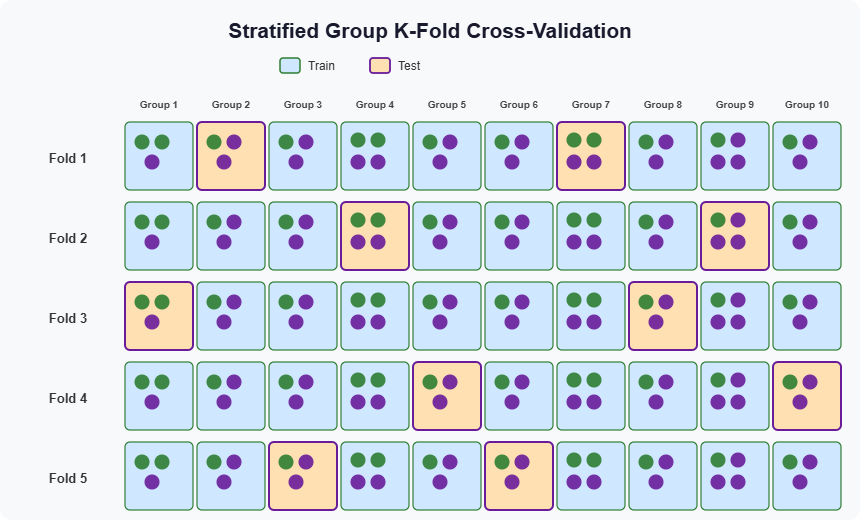
\includegraphics[width=0.82\textwidth]{images/stratified_group_k-fold_cv.png}
% \caption{\atc{Stratified group K-fold cross-validation. Stratification preserves class proportions across folds, whereas grouping reduces leakage between temporally neighbouring EEG trials.}}
% \label{fig:stratified-group-cv}
% \end{figure}

% \section{Classical and hypothesis-driven decoders}

% \atc{The first set of models used simple, hypothesis-driven EEG features. These models were motivated by the main effects observed in the previous analyses, especially frontal theta and occipital alpha modulations between congruent and incongruent images. For each trial, band-limited activity was extracted from predefined channels and frequency bands, summarized as scalar features, scaled within the training fold, and classified using L2-regularised logistic regression.}

% \atc{These models serve as interpretable baselines. If a single frontal theta or occipital alpha feature achieves above-chance decoding, the result is easy to relate to the time-frequency analyses. If these models fail, the failure is also informative because it suggests that the discriminative information is not captured by a single channel-band summary.}

% \atc{Additional classical classifiers were also evaluated on the same feature families. This classifier sweep was used to distinguish two questions: whether the selected representation contains discriminative information, and whether a more flexible classifier can exploit that information better. The purpose of this sweep was not to exhaustively optimise machine-learning performance, but to check whether the conclusions depended strongly on the choice of classifier.}

% \section{Riemannian covariance decoding}

% \atc{Riemannian covariance decoding was used as the main multichannel classical approach. Unlike single-feature models, covariance-based methods represent each trial through the relationships between EEG channels. This is appropriate for scalp EEG because condition-related information may be spatially distributed and mixed across sensors by volume conduction.}

% For each trial, the covariance matrix was computed as
% \begin{equation}
% C^{(i)} = \frac{1}{T-1}(X^{(i)}-\bar{X}^{(i)})(X^{(i)}-\bar{X}^{(i)})^\top,
% \end{equation}
% \atc{where $X^{(i)}$ is the multichannel EEG signal for trial $i$, and $T$ is the number of time samples. The covariance matrices were regularised using shrinkage and projected to the tangent space before classification with a linear classifier. The tangent-space projection allows covariance matrices to be analysed with standard linear methods while preserving the geometry of the covariance representation.}

% \atc{This model occupies an important position in the decoding hierarchy. It remains relatively simple and low-capacity, but it can capture distributed spatial structure that is invisible to single-electrode power summaries. Therefore, it provides a strong classical benchmark against which more flexible models can be compared.}

% \begin{figure}[H]
% \centering
% \resizebox{0.95\textwidth}{!}{%
% \begin{tikzpicture}[
% font=\small,
% >=Latex,
% node distance=1.6cm,
% box/.style={draw, rounded corners, align=center, minimum height=1.0cm, minimum width=2.5cm},
% smallbox/.style={draw, rounded corners, align=center, minimum height=0.9cm, minimum width=2.3cm},
% arrow/.style={->, thick}
% ]

% ```
%     \node[box] (epochs) {Balanced EEG epochs\\$N \times C \times T$};

%     \node[smallbox, above right=1.0cm and 2.0cm of epochs] (features) {Hypothesis-driven\\band-power features\\theta / alpha};
%     \node[smallbox, below right=1.0cm and 2.0cm of epochs] (cov) {Regularised covariance\\matrices\\$C \times C$};

%     \node[smallbox, right=2.3cm of features] (lr) {Logistic regression\\or classical ML};
%     \node[smallbox, right=2.3cm of cov] (lda) {Tangent space\\+ LDA};

%     \node[box, right=2.4cm of epochs] (eval) {Fold-contained\\evaluation\\balanced accuracy\\+ permutations};

%     \draw[arrow] (epochs.east) -- ++(0.7,0) |- (features.west);
%     \draw[arrow] (epochs.east) -- ++(0.7,0) |- (cov.west);

%     \draw[arrow] (features.east) -- (lr.west);
%     \draw[arrow] (cov.east) -- (lda.west);

%     \draw[arrow] (lr.east) -- ++(0.7,0) |- (eval.north);
%     \draw[arrow] (lda.east) -- ++(0.7,0) |- (eval.south);

% \end{tikzpicture}
% }
% \caption{\atc{Classical decoding pipelines. Hypothesis-driven band-power features and Riemannian covariance representations are treated as alternative feature spaces, not as sequential steps. All transformations are estimated within the training folds and evaluated on held-out data.}}
% \label{fig:classical-riemannian-pipeline}
% ```

% \end{figure}

% \section{Cluster-restricted decoding}

% \atc{Cluster-restricted classifiers were used to test whether sensor-time regions identified in the statistical analyses also contained discriminative information. These models used compact theta/alpha summaries extracted from selected cluster windows and classified them with a support vector classifier or related classical models.}

% \atc{These analyses should be interpreted as exploratory unless the cluster selection is performed independently of the decoding evaluation. If the same dataset is used first to identify a cluster and then to estimate decoding performance within that cluster, the performance estimate may be optimistic because the feature space has already been selected using condition-related information. A confirmatory cluster-restricted analysis would require either clusters defined from a previous study or cluster selection performed separately within each training fold.}

% \section{Deep-learning baselines}

% \atc{Deep-learning models were included as exploratory baselines to test whether learned spatio-temporal representations improved decoding beyond the classical approaches. Because the dataset is limited and the decoding contrasts are subtle, these models were not treated as the primary evidence of the thesis. Their role was to provide a comparison with modern EEG architectures under the same validation constraints.}

% \atc{The main compact neural-network baseline was EEGNet. EEGNet combines temporal convolutions, depthwise spatial filtering, separable convolutions, pooling, dropout, and a small classification head. Conceptually, this resembles a learned version of temporal filtering followed by spatial projection, making it a useful lightweight EEG-specific baseline.}

% \atc{A spatio-temporal graph neural network was also evaluated. This model represents electrodes as nodes in a spatial graph and uses graph convolution followed by temporal processing. It tests whether incorporating the scalp montage structure helps decoding.}

% \atc{Finally, ST-EEGFormer and LaBraM were included as pretrained or foundation-model-style EEG baselines with parameter-efficient fine-tuning. Their motivation is that representations learned from large EEG corpora might transfer to the present task. However, their use involves practical constraints such as channel mapping, resampling, tokenisation, and possible mismatch between the pretraining objective and the binocular-rivalry paradigm. For this reason, these models were treated as exploratory comparisons rather than as central methodological contributions.}

% \atc{The detailed architecture diagrams for EEGNet, ST-GNN, ST-EEGFormer, and LaBraM are not included in the main chapter because the central methodological result is not a new neural-network architecture. If needed, these diagrams can be moved to an appendix as implementation documentation.}

% \section{Configuration search and model selection}

% \atc{The decoding analysis also examined how preprocessing and representation choices affected performance. The relevant object of comparison was the complete pipeline, not only the final classifier. Choices such as frequency band, time window, channel set, scaling strategy, covariance representation, and model family can all influence decoding performance.}

% \atc{This configuration search was used to understand the sensitivity of the results to analysis choices. However, it should not be interpreted as an unrestricted optimisation procedure unless the selected configuration is evaluated on an independent holdout set or within a nested cross-validation framework. Otherwise, repeated comparison of many pipelines can lead to optimistic performance estimates.}

% \section{Interpretability analysis}

% \atc{Interpretability analyses were used as diagnostics of model behaviour, not as independent evidence for neural mechanisms. Their purpose was to check whether models that achieved above-chance performance relied on channels, time windows, or frequency components compatible with the frontal theta and occipital alpha effects observed in the statistical analyses.}

% \atc{For deep-learning models, feature attribution was estimated using Integrated Gradients. This method compares the model output for an observed EEG trial with the output for a reference baseline and integrates the input gradients along the path from the baseline to the observed input. In this thesis, attribution maps were used to summarize which parts of the sensor-time input influenced the model prediction.}

% \atc{These maps were interpreted cautiously. Attribution depends on the trained model, the preprocessing pipeline, the baseline choice, and the stability of the classifier. A visually structured attribution map from a model performing near chance should not be interpreted as physiological evidence. Attribution was therefore considered meaningful only when it converged with decoding performance and with independent EEG evidence from the time-frequency, topographic, and cluster-based analyses.}

% \atc{For classical models, interpretability was based on the features used by the model itself. Logistic-regression baselines were interpreted through their predefined frontal theta or occipital alpha features. Riemannian covariance decoding was interpreted as evidence for distributed multichannel structure. Cluster-restricted models were interpreted through the selected sensor-time regions, with the circularity caveat described above.}

\chapter{Decoding Results}
\label{chap:results}

\section{Task-Level Decoding Patterns}

As summarized in Table~\ref{tab:balanced-accuracy}, the decoding analyses showed a clear difference between the two classification tasks. C vs IP was the more reliable contrast, whereas IM vs IP remained close to chance for most models. This distinction matters because the two tasks do not test the same type of information. C vs IP compares compatible trials with incompatible trials that still lead to a single-color report, and therefore provides the cleaner test of interocular conflict. IM vs IP compares mixed and single-color reports within incompatible stimulation, making it a more subtle and exploratory contrast.

The absolute decoding accuracies were modest. This is expected for single-trial scalp EEG in a subtle perceptual task, and the results should not be interpreted as strong individual-trial prediction. Instead, the relevant question is whether performance is consistently above chance under conservative validation and whether the strongest models point to physiologically plausible representations. Under this interpretation, the C vs IP results provide evidence for weak but structured discriminative information.

For C vs IP, the strongest performance was obtained with Riemannian covariance features combined with LDA. This suggests that the useful information is not fully captured by a single fronto-medial theta or parieto-occipital alpha feature, but is better represented as distributed multichannel structure. The experiment-guided classical model and the cluster-restricted SVC also performed above the simplest single-feature baselines, supporting the view that representation choice is central to the decoding result.

For IM vs IP, most models remained close to chance. The best value was obtained with the cluster-restricted SVC, but the margin over other models was small. This should therefore be interpreted as evidence that IM vs IP is unstable in the present dataset, rather than as strong evidence for one specific classifier. This weaker result is scientifically plausible: both IM and IP trials involve incompatible stimulation, and the distinction depends on the subjective perceptual report rather than on a clean physical stimulus difference.

Thus, the contrast between C vs IP and IM vs IP is one of the main findings of the decoding analysis. C vs IP provides limited but interpretable evidence for conflict-related EEG information, whereas IM vs IP remains exploratory.

\section{Model Comparison}

Table~\ref{tab:balanced-accuracy} summarizes the final balanced-accuracy comparison. The main result is that increasing model complexity did not systematically improve decoding. Classical and Riemannian approaches performed at least as well as, and in some cases better than, compact neural networks and pretrained foundation-model adaptations. This suggests that the limiting factor is not simply classifier expressivity, but the combination of signal-to-noise ratio, subject variability, feature representation, and validation constraints.

\begin{table}[H]
    \centering
    \caption{Reserved final-holdout balanced accuracy summary. Values are mean $\pm$ standard deviation across subjects, rounded to the nearest tenth of a percentage point.}
    \label{tab:balanced-accuracy}
    \small
    \begin{tabularx}{\textwidth}{@{}lcc@{}}
        \toprule
        Model                          & C vs IP Balanced Accuracy (\%) & IM vs IP Balanced Accuracy (\%) \\
        \midrule
        Logistic regression, FCz-theta & 49.6 $\pm$ 6.7                 & 50.6 $\pm$ 8.6                  \\
        Logistic regression, Oz-alpha  & 53.6 $\pm$ 8.2                 & 49.4 $\pm$ 8.0                  \\
        Riemannian covariance + LDA    & \textbf{58.7 $\pm$ 8.3}        & 49.3 $\pm$ 6.1                  \\
        Experiment-guided classical ML & 56.9 $\pm$ 8.1                 & 50.9 $\pm$ 8.1                  \\
        SVC cluster features           & 56.2 $\pm$ 6.3                 & \textbf{52.7 $\pm$ 6.2}         \\
        EEGNet agnostic                & 53.2 $\pm$ 8.2                 & 49.5 $\pm$ 5.8                  \\
        EEGNet clustering              & 49.6 $\pm$ 8.0                 & 48.5 $\pm$ 7.5                  \\
        ST-GNN                         & 52.0 $\pm$ 7.3                 & 51.4 $\pm$ 5.6                  \\
        ST-EEGFormer                   & 52.5 $\pm$ 8.3                 & 50.7 $\pm$ 5.8                  \\
        LaBraM adaptation              & 51.9 $\pm$ 6.8                 & 48.2 $\pm$ 9.6                  \\
        \bottomrule
    \end{tabularx}
\end{table}

For C vs IP, the best model was Riemannian covariance + LDA, reaching $58.7\%$ balanced accuracy. This was followed by the experiment-guided classical model and the SVC trained on cluster-derived features. For IM vs IP, the best value was obtained with the cluster-restricted SVC, but the absolute performance remained low at $52.7\%$. This contrast supports the interpretation that C vs IP contains more stable discriminative information than IM vs IP.

The deep-learning models did not clearly outperform the classical baselines. EEGNet, ST-GNN, ST-EEGFormer, and LaBraM remained close to chance or only modestly above it. These models should therefore be treated as exploratory comparisons rather than as central evidence. Their weak performance is nevertheless informative, because it shows that larger or more flexible models do not automatically improve decoding in this dataset.

The cluster-restricted SVC result should also be interpreted cautiously. If the clusters used to define the features were selected using the full dataset, the decoding estimate may be optimistic because the same data contributed to feature selection and performance evaluation. A confirmatory version of this analysis would require cluster selection inside each training fold, or clusters defined from an independent dataset or previous study.

The ROC and precision--recall curves in Figure~\ref{fig:cohort-roc-pr-curves} complement the accuracy table. The table gives a compact ranking, while the curves show whether the ranking reflects a consistent discrimination trade-off or only a single threshold choice.

\begin{figure}[H]
    \centering
    \panelimage{0.48\textwidth}{images/cohort_roc_pr_curves_c_vs_ip.png}{C vs IP cohort ROC and precision--recall curves.}
    \hfill
    \panelimage{0.48\textwidth}{images/cohort_roc_pr_curves_im_vs_ip_comparison.png}{IM vs IP cohort ROC and precision--recall curves.}
    \caption{Cohort-level discrimination curves for the two binary tasks. C vs IP shows the clearer above-chance pattern, led by Riemannian covariance, whereas IM vs IP remains close to chance for most models.}
    \label{fig:cohort-roc-pr-curves}
\end{figure}

The C vs IP curves separate more clearly than the IM vs IP curves, supporting the task-level interpretation. Riemannian covariance is not only the best row in Table~\ref{tab:balanced-accuracy}; it also has the cleanest cohort-wide curve profile for C vs IP. By contrast, the IM vs IP curves remain clustered near chance, reinforcing the view that this task is exploratory.

\section{Pipeline and Configuration Effects}

The configuration analyses indicate that decoding performance depends on the complete analysis pipeline, not only on the final classifier. Choices such as frequency band, time window, channel set, scaling strategy, covariance representation, and model family can all influence performance. This is particularly important in low-SNR EEG, where small preprocessing choices may determine whether a weak effect is preserved or removed.

For C vs IP, the best-performing configuration favored distributed covariance-based decoding, consistent with the idea that the relevant information is spatially distributed rather than restricted to a single electrode. For IM vs IP, the best-performing configuration was more constrained and alpha/ROI-based, but the overall decoding performance remained weak. This reinforces the interpretation that IM vs IP is exploratory.

\begin{figure}[H]
    \centering
    \panelimage{0.55\textwidth}{images/experiment8_marginal_component_means.png}{Marginal accuracy by component value.}
    \hfill
    \panelimage{0.42\textwidth}{images/experiment10_component_contributions.png}{One-at-a-time component contributions.}
    \caption{Configuration-search summaries. The results indicate that preprocessing, spatial scope, spectral representation, temporal window, and classifier family jointly shape decoding performance.}
    \label{fig:configuration-search-summaries}
\end{figure}

Figure~\ref{fig:configuration-search-summaries} should be interpreted as a methodological diagnostic rather than as an independent confirmatory result. It shows why model family cannot be evaluated separately from the representation provided to the model. However, because many configurations were searched on the same dataset, the selected configuration may be optimistic unless evaluated using a nested procedure or an independent holdout set.

\subsection{Training and Temporal-Generalization Diagnostics}

The last result-level diagnostics in Figure~\ref{fig:training-and-tgm-diagnostics} check two possible failure modes. The EEGNet history asks whether the neural baseline is simply undertrained or unstable. The temporal generalization matrix asks whether decoding learns a representation that transfers across time, or whether it is tied to local temporal windows.

\begin{figure}[H]
    \centering
    \panelimage{0.6\textwidth}{images/training_history_c_vs_ip_eegnet.png}{EEGNet training history for C vs IP.}
    \hfill
    \panelimage{0.35\textwidth}{images/tgm_matrix_only.png}{Temporal generalization matrix.}
    \caption{Training and temporal-generalization diagnostics. The EEGNet history confirms modest learning without a large validation jump, and the temporal generalization matrix shows that decoding is mostly local in time rather than a stable representation that transfers across the whole trial.}
    \label{fig:training-and-tgm-diagnostics}
\end{figure}

Both diagnostics support the conservative interpretation. EEGNet learns something, but not enough to overtake the classical baselines, and the temporal-generalization map is mostly near-diagonal rather than broadly transferable. This fits the broader claim that the available signal is weak, local, and representation-sensitive.

\section{Interpretability}
The interpretability analyses were used as diagnostics of model behavior, not as independent evidence for neural mechanisms. Their purpose was to check whether models with above-chance performance relied on channels and time windows compatible with the theta/alpha effects observed in the previous analyses. The attribution summaries were therefore computed on the subset of subjects whose decoding performance was above a minimal task-specific threshold: 55\% balanced accuracy for C vs IP and 53\% for IM vs IP.\footnote{The thresholds are intentionally modest because the single-trial accuracies are modest overall. They are used only to avoid averaging attribution maps from clearly near-chance models; they are not statistical significance cutoffs and do not turn attribution into confirmatory neural evidence.} These thresholds do not make the attribution results confirmatory, but they reduce the risk of interpreting maps from models that are essentially guessing.

The attribution notebooks export three complementary visual checks for each contrast. The spatial maps compare electrode-level importance across the reliable subject cohort, the temporal curves show when each model places most of its relevance within the analyzed window, and the consensus diagnostic combines the separate summaries into a compact agreement view. These plots should not be read as source-localization results; they are sensor-level model-behavior diagnostics.

For C vs IP, the attribution results are most informative because this is the stronger decoding task. The spatial maps do not point to a single isolated electrode. The hypothesis-driven baselines recover their expected anchors, with a focal FCz channel theta map and a focal Oz channel alpha map, but the stronger multichannel models spread importance over broader posterior and central-posterior sensors, with a smaller fronto-medial component. This pattern matches the earlier statistical results: posterior alpha is the clearest and broadest effect, while fronto-medial theta is present but narrower.

\begin{figure}[H]
    \centering
    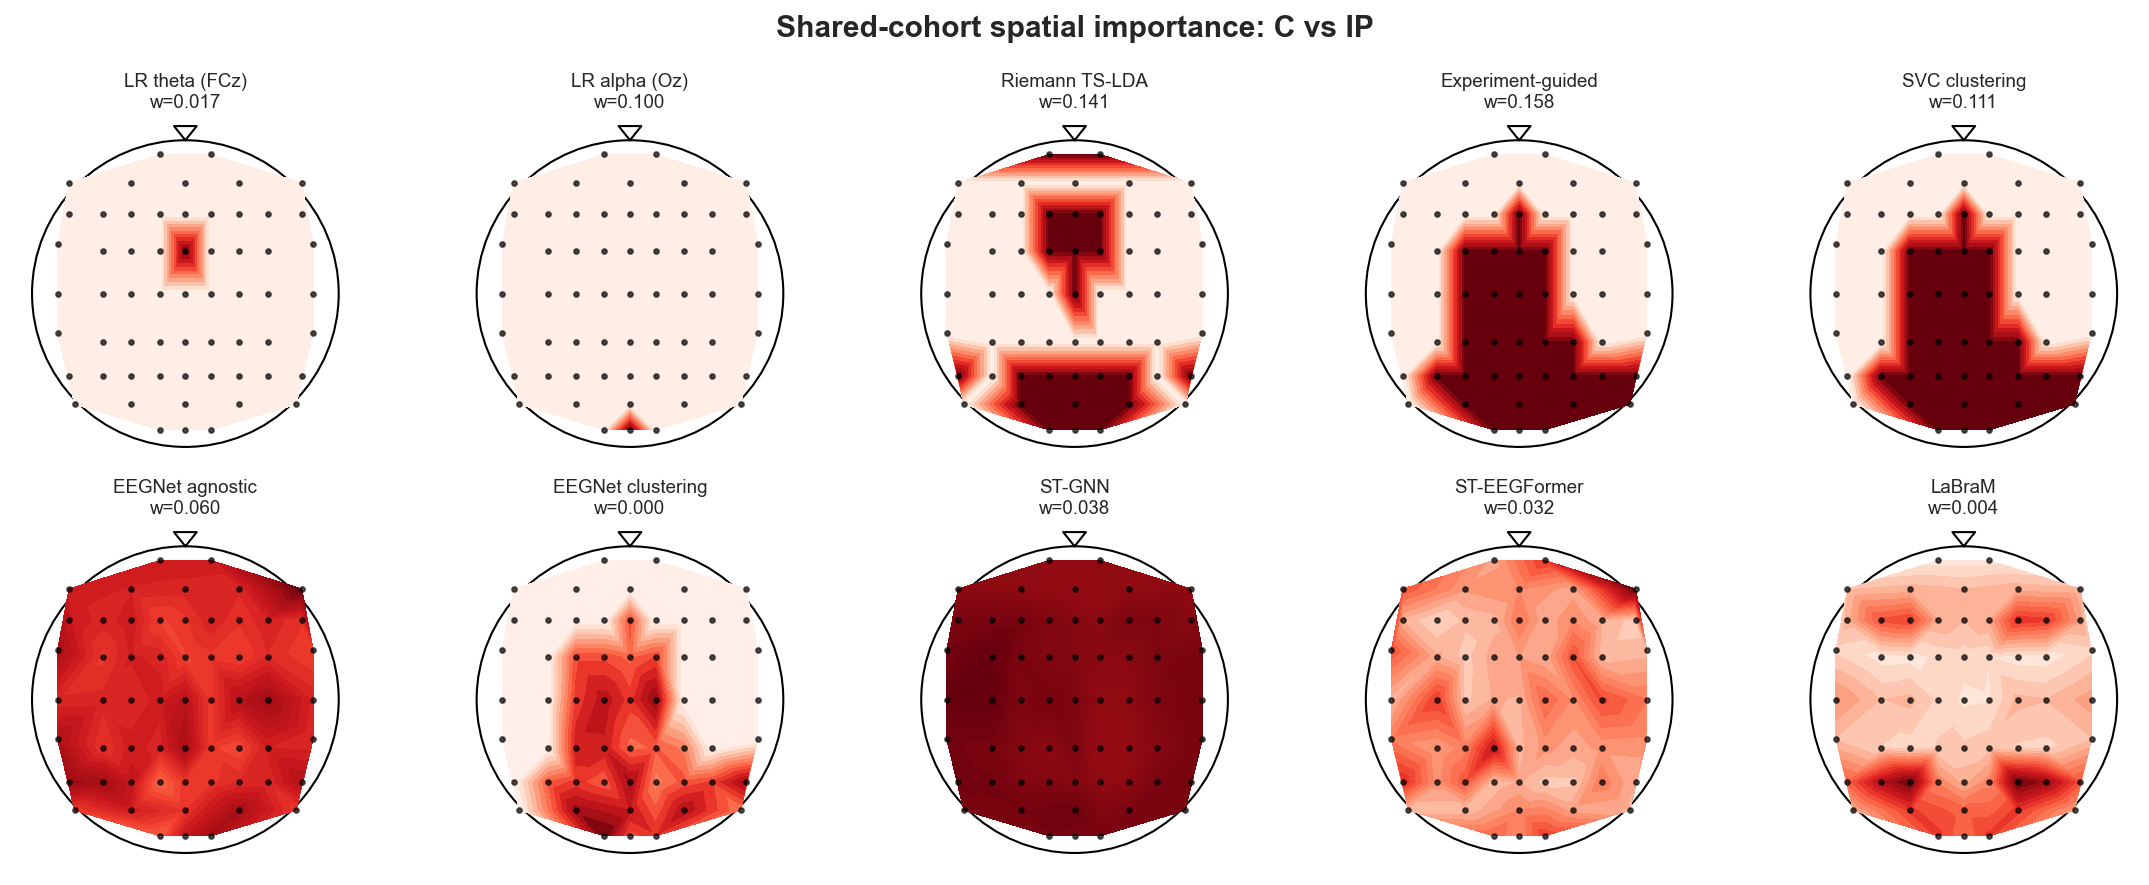
\includegraphics[width=0.96\textwidth]{images/shared_cohort_spatial_topomaps_c_vs_ip.png}
    \caption{Shared-cohort spatial attribution for C vs IP. The maps are interpreted as sensor-level diagnostics of model behavior, not as source-localization results.}
    \label{fig:attr-spatial-cvip}
\end{figure}

The temporal attribution curves add the time dimension to the same pattern. The Oz-alpha baseline shows a broad mid-to-late peak, centered roughly around 0.7--0.8 s, rather than a brief onset response. The flexible models distribute relevance across wider parts of the epoch, with several curves remaining elevated into later windows. This supports the idea that C vs IP decoding is not driven by a single instantaneous feature, but by sustained sensor-level information over the post-stimulus interval.

\begin{figure}[H]
    \centering
    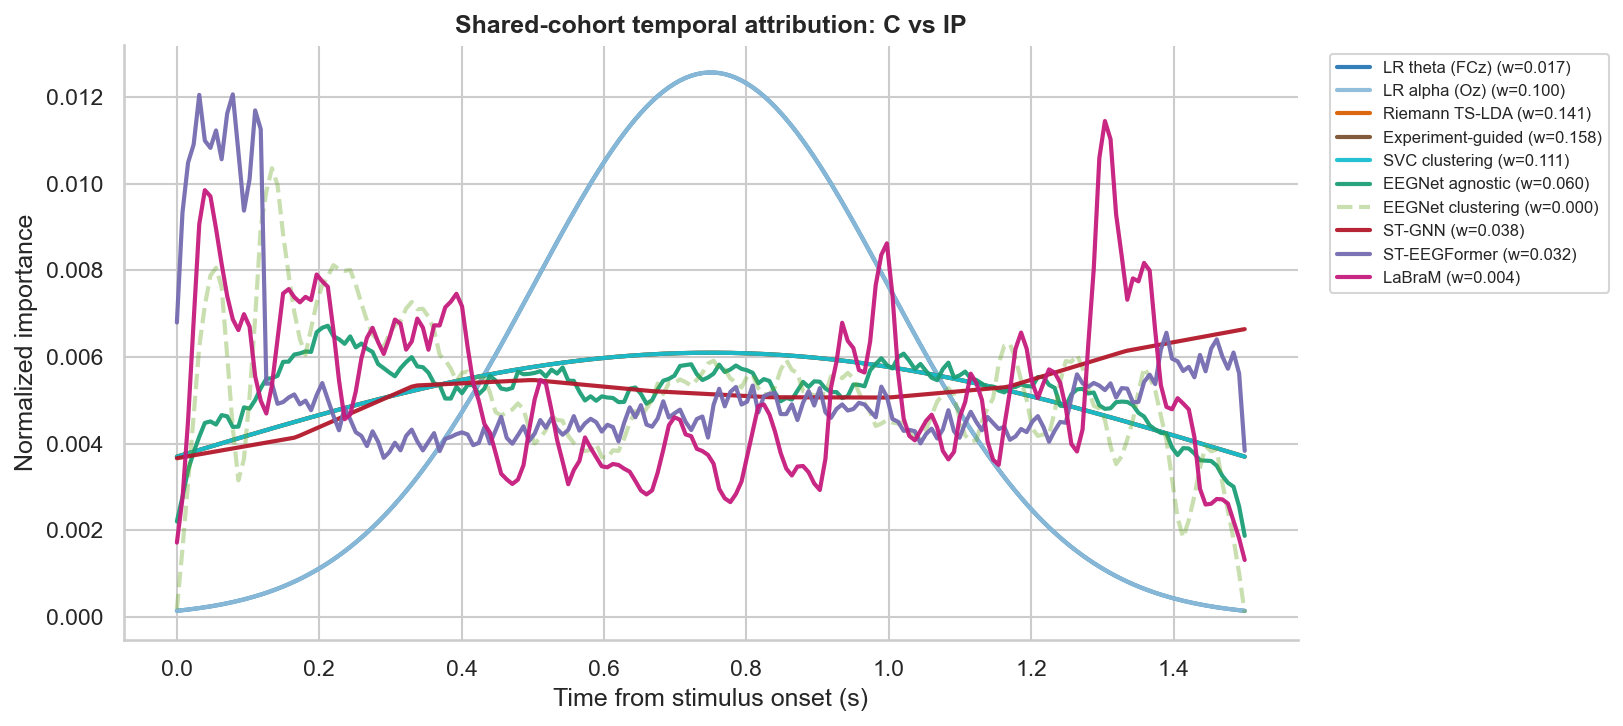
\includegraphics[width=0.90\textwidth]{images/shared_cohort_temporal_attribution_c_vs_ip.png}
    \caption{Shared-cohort temporal attribution for C vs IP. The curves show when each model places relevance within the analyzed trial window, making it possible to compare late alpha/theta windows against the model-behavior evidence.}
    \label{fig:attr-temporal-cvip}
\end{figure}

The C vs IP consensus diagnostic summarizes this convergence. Spatially, the weighted map is centered on a broad posterior and central-posterior pattern rather than on the FCz channel alone. Temporally, the consensus curve rises after stimulus onset and stays elevated across much of the analyzed window, with several local maxima before declining near the end of the epoch. The consensus therefore supports the same interpretation as the model comparison: C vs IP contains a weak but structured distributed signal, with posterior alpha and multichannel covariance carrying more usable information than a single theta trace.

\begin{figure}[H]
    \centering
    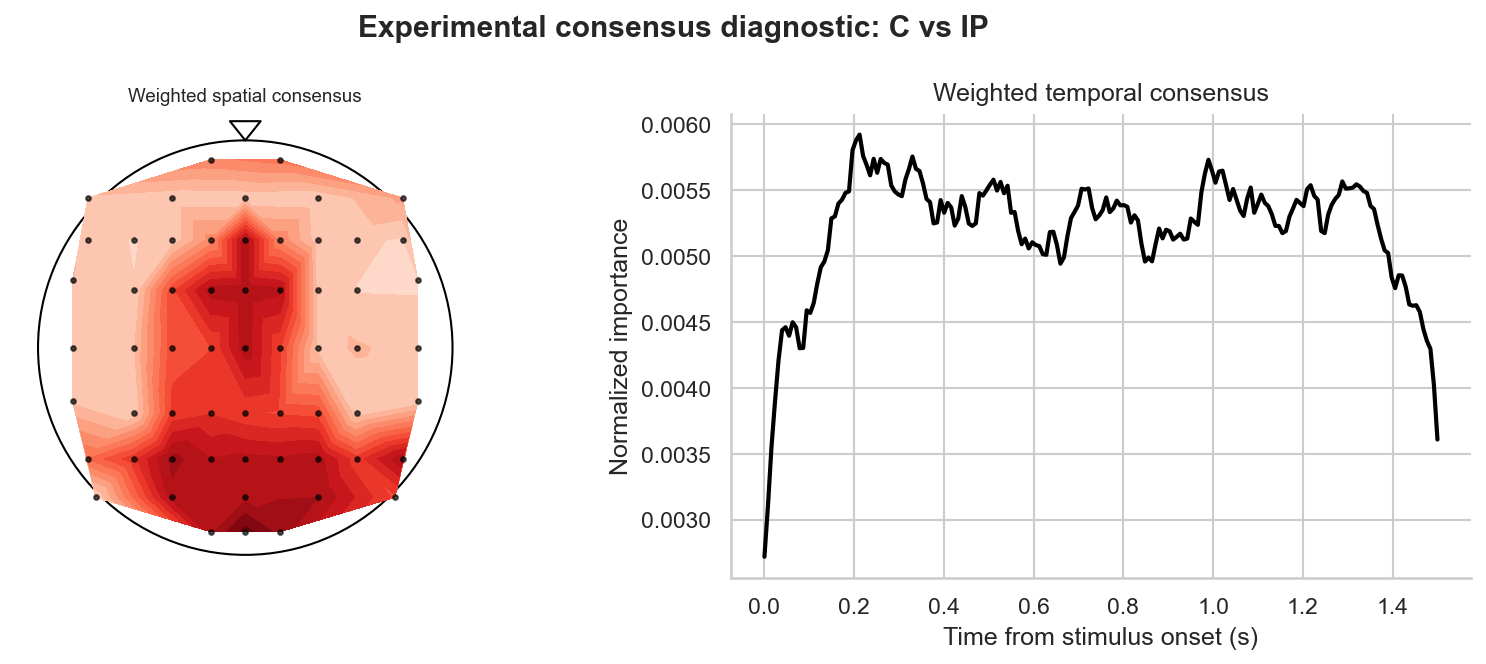
\includegraphics[width=0.90\textwidth]{images/experimental_consensus_diagnostic_c_vs_ip.png}
    \caption{Consensus diagnostic for C vs IP, combining weighted spatial and temporal model attribution into a compact agreement check.}
    \label{fig:attr-consensus-cvip}
\end{figure}

IM vs IP shows a weaker and less consistent attribution profile, but it is still informative as a diagnostic of the models that exceed the 53\% threshold. The spatial maps again show the expected focal anchors for the simple theta and alpha baselines, while the multichannel and cluster-guided models emphasize a more mixed pattern. The clearest repeated structure is not a clean posterior alpha pattern like C vs IP, but a combination of central/fronto-central relevance and a left posterior extension. This fits the harder nature of the contrast: both classes come from incongruent stimulation, and the label separates mixed from single-color reports rather than conflict from no conflict.

\begin{figure}[H]
    \centering
    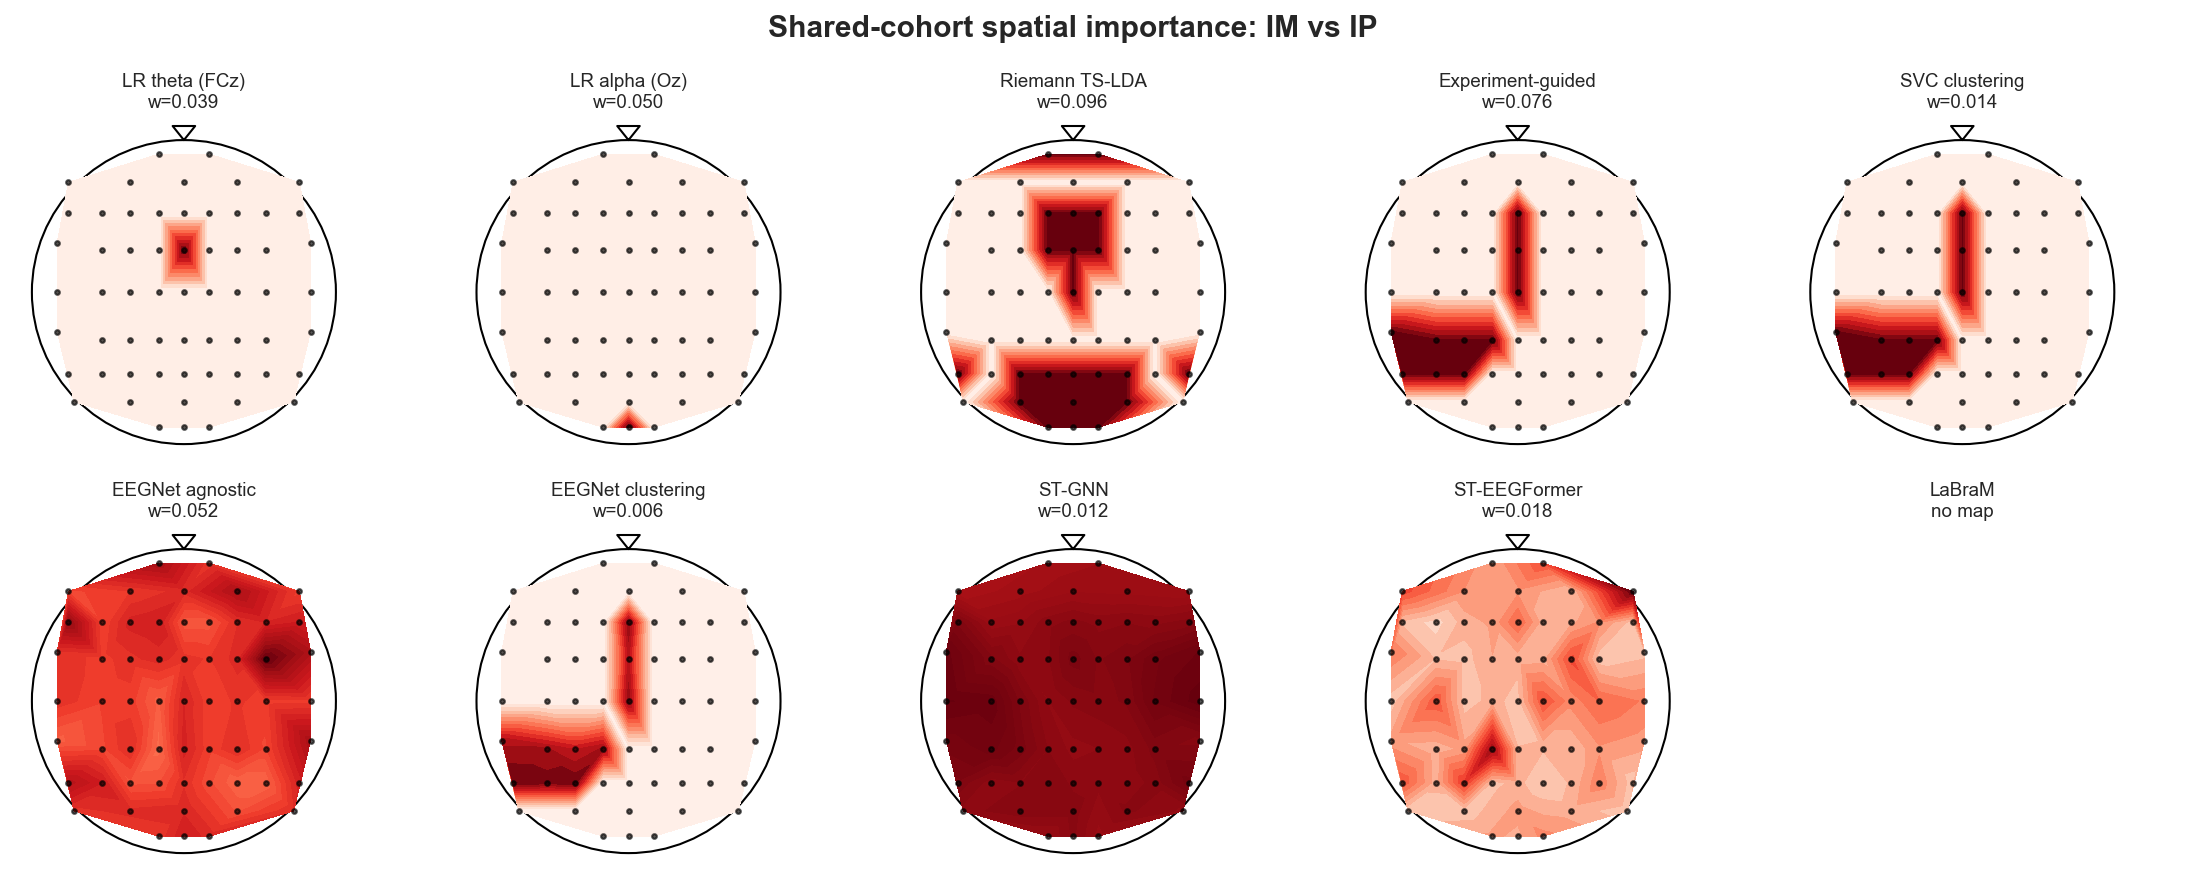
\includegraphics[width=0.96\textwidth]{images/shared_cohort_spatial_topomaps_im_vs_ip.png}
    \caption{Shared-cohort spatial attribution for IM vs IP. The maps are weaker and less consistent than C vs IP, but they are still useful for checking which sensor regions are used by above-threshold models.}
    \label{fig:attr-spatial-imip}
\end{figure}

The IM vs IP temporal curves also differ from C vs IP. The Oz-alpha baseline has a broad peak around the middle of the epoch, while several learned models show flatter or more irregular relevance over time. The consensus curve increases through the first half of the window, reaches its strongest values around 0.9--1.0 s, and then declines. This late emphasis is compatible with the idea that IM vs IP depends on a more variable perceptual outcome, but the evidence is not as coherent as the C vs IP pattern.

\begin{figure}[H]
    \centering
    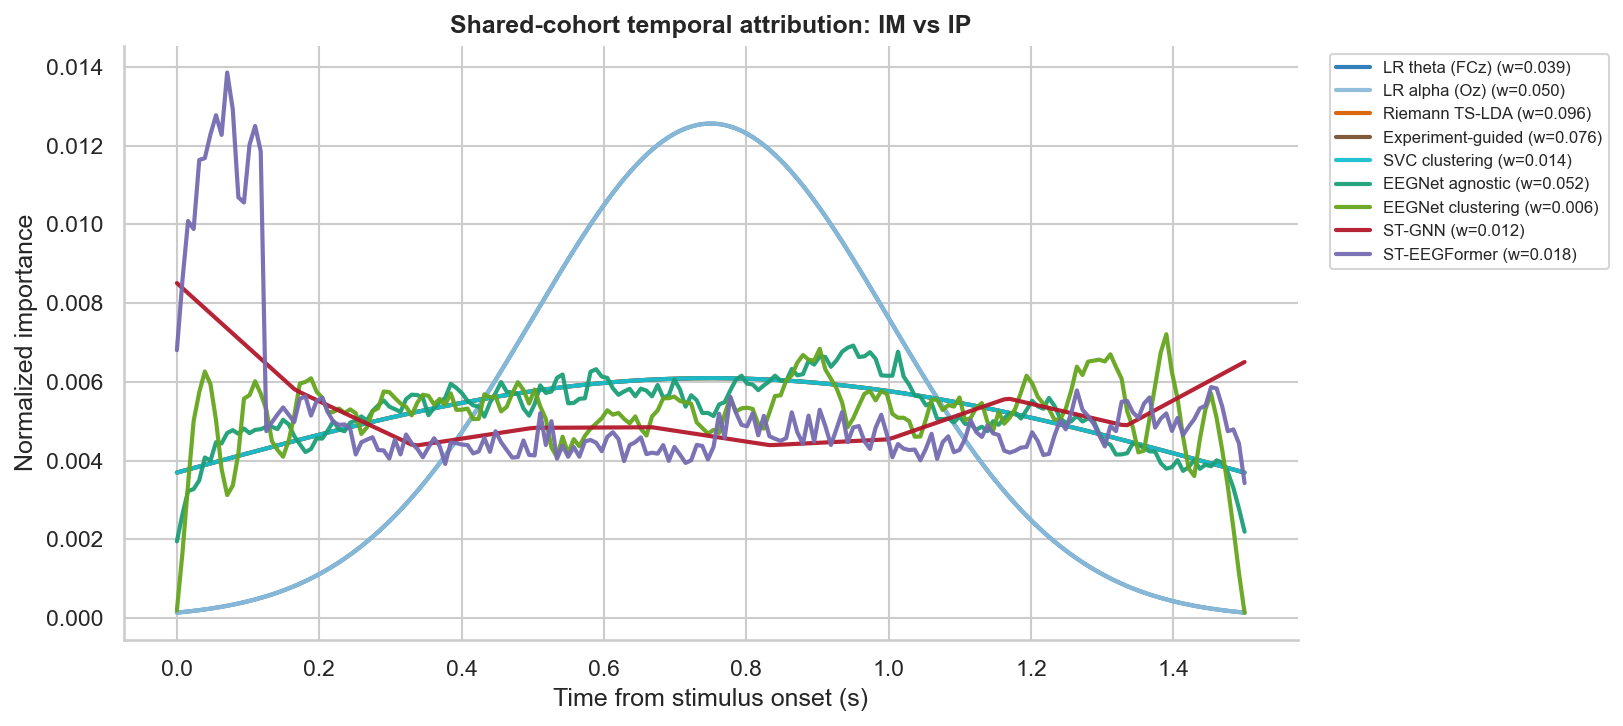
\includegraphics[width=0.90\textwidth]{images/shared_cohort_temporal_attribution_im_vs_ip.png}
    \caption{Shared-cohort temporal attribution for IM vs IP. Compared with C vs IP, the curves show weaker agreement across models and a less sharply defined temporal profile.}
    \label{fig:attr-temporal-imip}
\end{figure}

\begin{figure}[H]
    \centering
    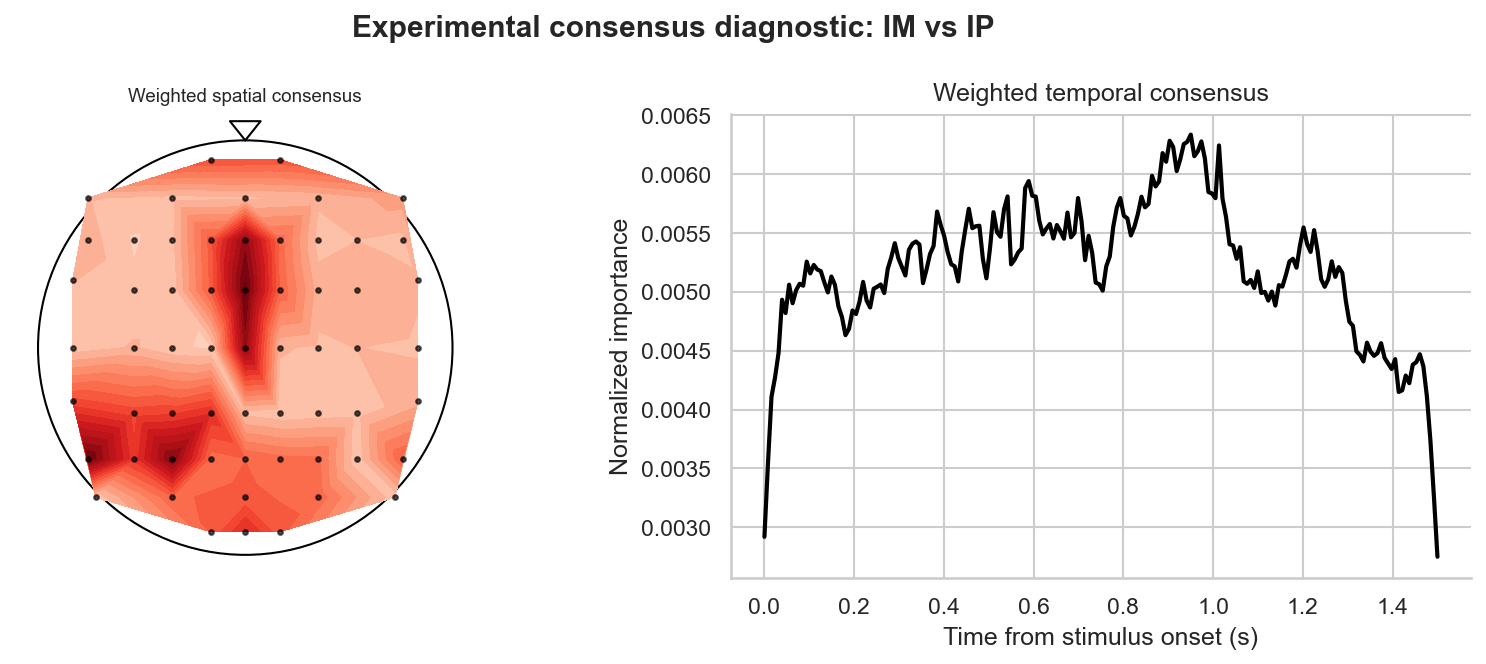
\includegraphics[width=0.90\textwidth]{images/experimental_consensus_diagnostic_im_vs_ip.png}
    \caption{Consensus diagnostic for IM vs IP. The weighted summary suggests a weaker fronto-central and left posterior pattern, with temporal relevance peaking later in the analyzed window.}
    \label{fig:attr-consensus-imip}
\end{figure}

Taken together, the attribution results support a graded interpretation of the two contrasts. C vs IP shows the clearest alignment between decoding, clustering, and model relevance: the models that work best tend to use distributed posterior and central-posterior information over a sustained post-stimulus interval. IM vs IP does not collapse into random noise, but its maps are less stable and its temporal profile is less sharply tied to the theta/alpha story. For this reason, the interpretability results are used to audit whether the decoding models behave plausibly, while the main neural interpretation remains anchored in the convergence between replication, clustering, decoding performance, and attribution. Source-like cortical projection figures are not used as main evidence in this chapter, because the thesis analyses sensor-level scalp EEG rather than source-localized activity.

% The strongest interpretable pattern remains posterior alpha and distributed covariance for C vs IP. Neural-model attribution is more fragile than the classical-model statistics, but its intended role is clear: check whether model-relevant channels and windows agree with the cluster-based theta/alpha evidence. For C vs IP, attribution should therefore be read as supporting evidence only when it converges with the posterior alpha cluster, the fronto-medial theta hypothesis, and the models that are demonstrably above chance. For IM vs IP, attribution is mostly diagnostic because the decoding benchmark itself is weaker.

% The attribution notebooks export three complementary visual checks for each task. The spatial maps compare electrode-level importance across the reliable subject cohort. The temporal curves show when each model places most of its relevance within the analysed window. The peak-time or consensus diagnostic compresses the separate spatial and temporal summaries into a comparison view, making it easier to see whether model families agree or whether a model appears to rely on a task-irrelevant pattern. These plots should not be read as source-localisation results; they are sensor-level model-behaviour diagnostics.

% For C vs IP, the spatial attribution panel supports the same cautious conclusion as the clustering results: the useful information is not a single isolated electrode, and the strongest classical models point toward broader posterior and central-posterior structure. Some deep-model maps are diffuse or noisy, which is expected when their decoding performance is only modest. They are useful because disagreement itself is informative: attribution is strongest evidence only when it converges with both performance and the independent theta/alpha statistics.

% \begin{figure}[H]
%     \centering
%     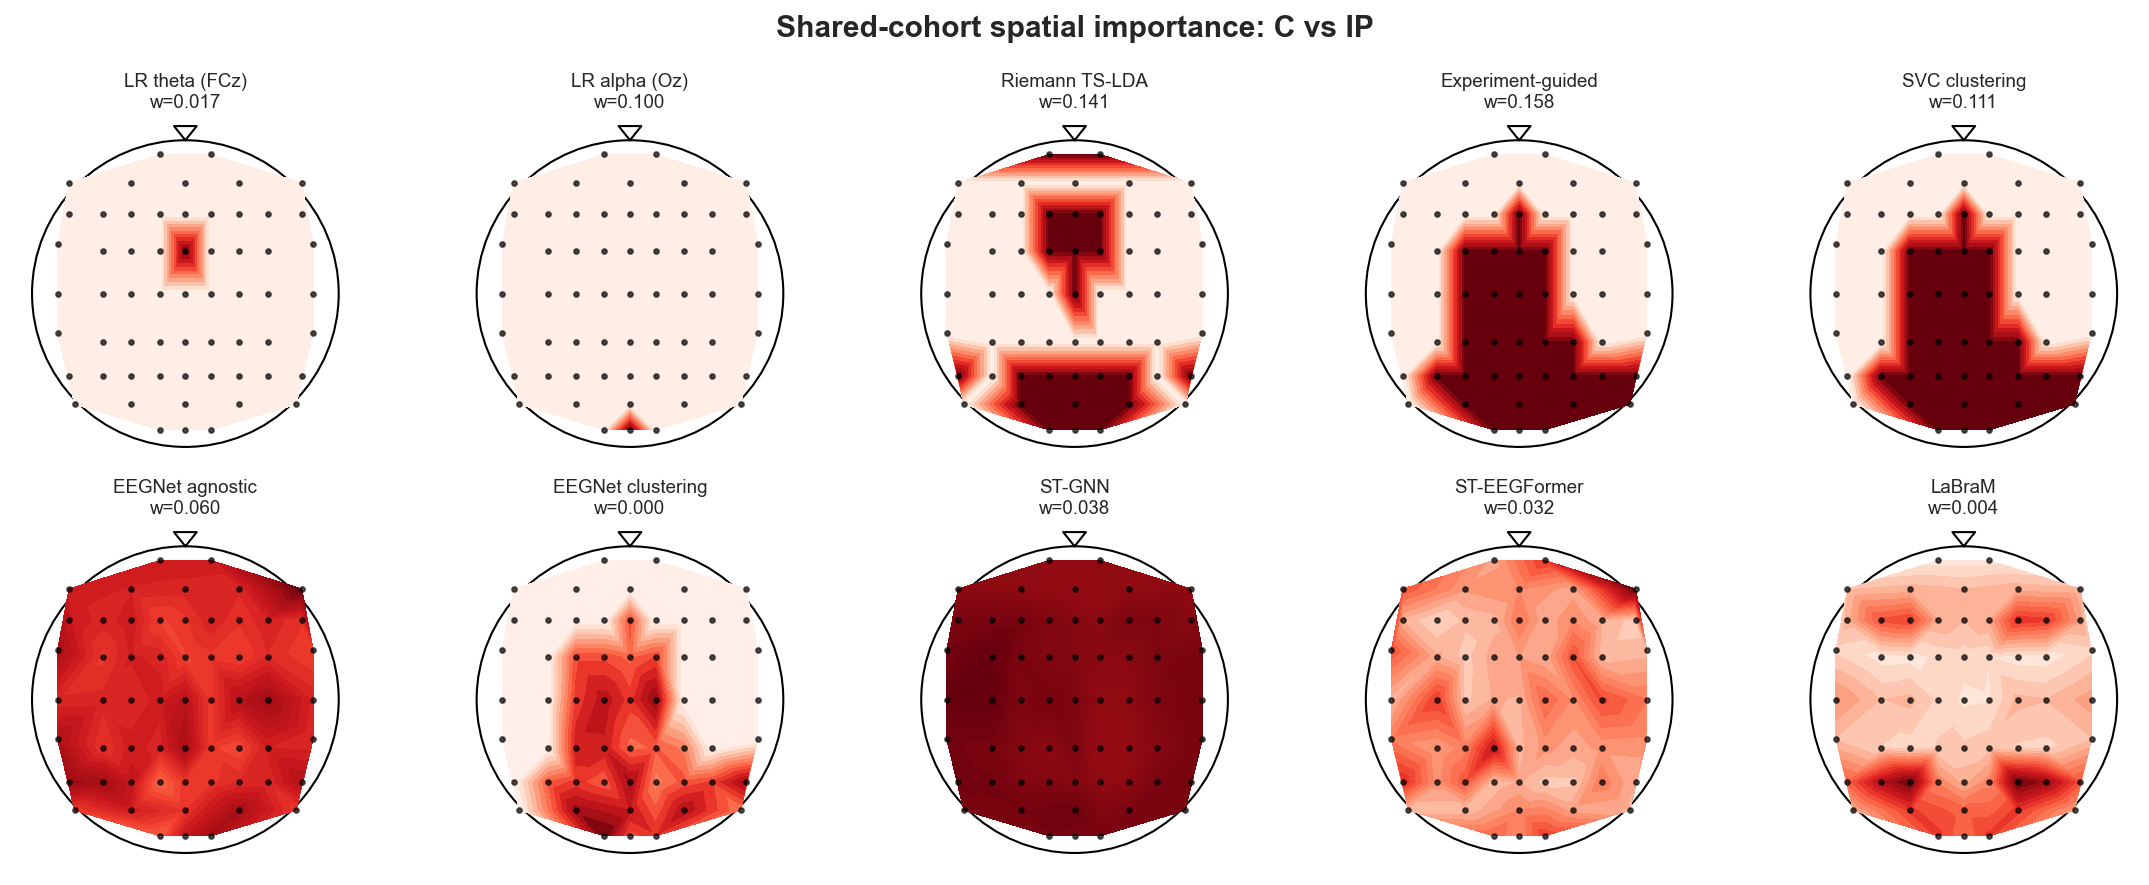
\includegraphics[width=0.96\textwidth]{images/shared_cohort_spatial_topomaps_c_vs_ip.png}
%     \caption{Shared-cohort spatial attribution for C vs IP. Each topomap is a sensor-level importance diagnostic for one model family; darker red indicates stronger normalized contribution within the shared cohort summary.}
%     \label{fig:attr-spatial-cvip}
% \end{figure}

% The C vs IP spatial maps are most useful when read against the clustering chapter. The classical and cluster-guided models place importance on plausible theta/alpha regions, while the neural maps are more heterogeneous. That heterogeneity is not a contradiction; it is one reason the thesis avoids treating any single attribution map as a final explanation.

% \begin{figure}[H]
%     \centering
%     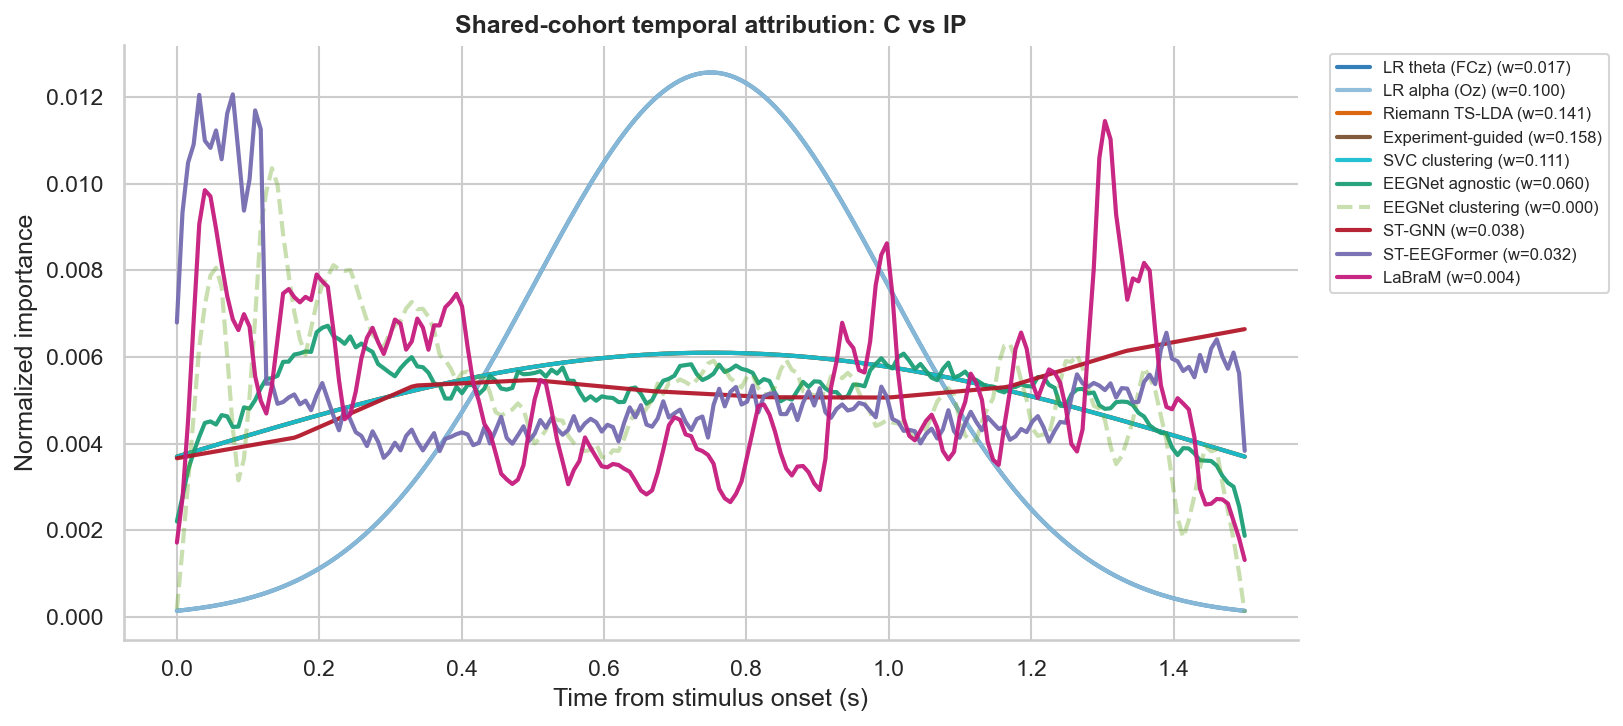
\includegraphics[width=0.90\textwidth]{images/shared_cohort_temporal_attribution_c_vs_ip.png}
%     \caption{Shared-cohort temporal attribution for C vs IP. The curves show when each model places relevance within the analysed trial window, making it possible to compare late alpha/theta windows against the model-behaviour evidence.}
%     \label{fig:attr-temporal-cvip}
% \end{figure}

% The temporal attribution curves add the time dimension to the same check. They do not reproduce the condition-average power curves exactly, because attribution measures model relevance rather than raw signal difference. Their value is that several stronger models place relevance in late windows compatible with the cluster and time-power evidence.

% \begin{figure}[H]
%     \centering
%     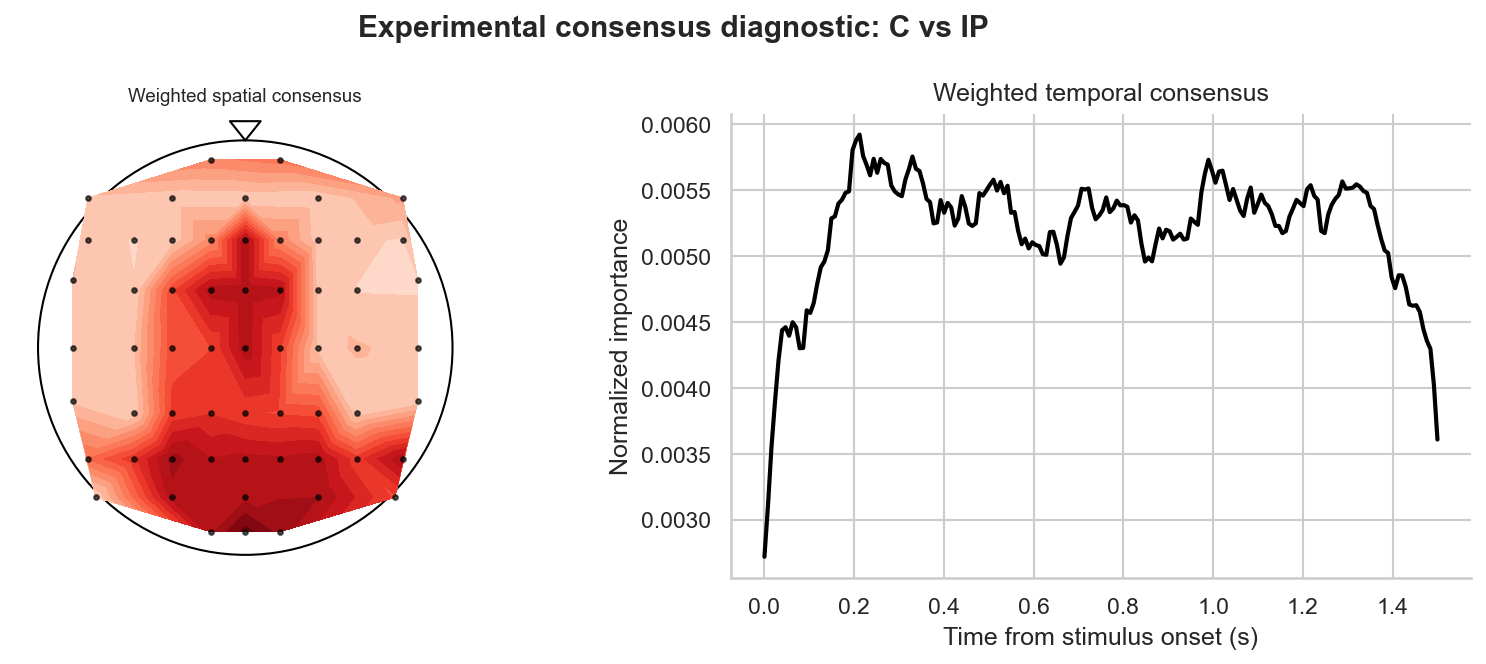
\includegraphics[width=0.90\textwidth]{images/experimental_consensus_diagnostic_c_vs_ip.png}
%     \caption{Consensus diagnostic for C vs IP, combining weighted spatial and temporal model attribution into a compact agreement check.}
%     \label{fig:attr-consensus-cvip}
% \end{figure}

% The consensus diagnostic is a compact audit view. It is kept in the main text because C vs IP is the stronger task: the attribution summary is interpretable only because there is already independent evidence from clusters and decoding performance.

% The IM vs IP attribution figures are included mainly to show what weaker evidence looks like. The plots still contain structured peaks and spatial patterns, but those patterns do not have the same support from decoding performance or cluster stability. This is why the thesis treats IM vs IP as exploratory: the interpretability outputs are not ignored, but they are not allowed to overrule the weaker benchmark.

% \begin{figure}[H]
%     \centering
%     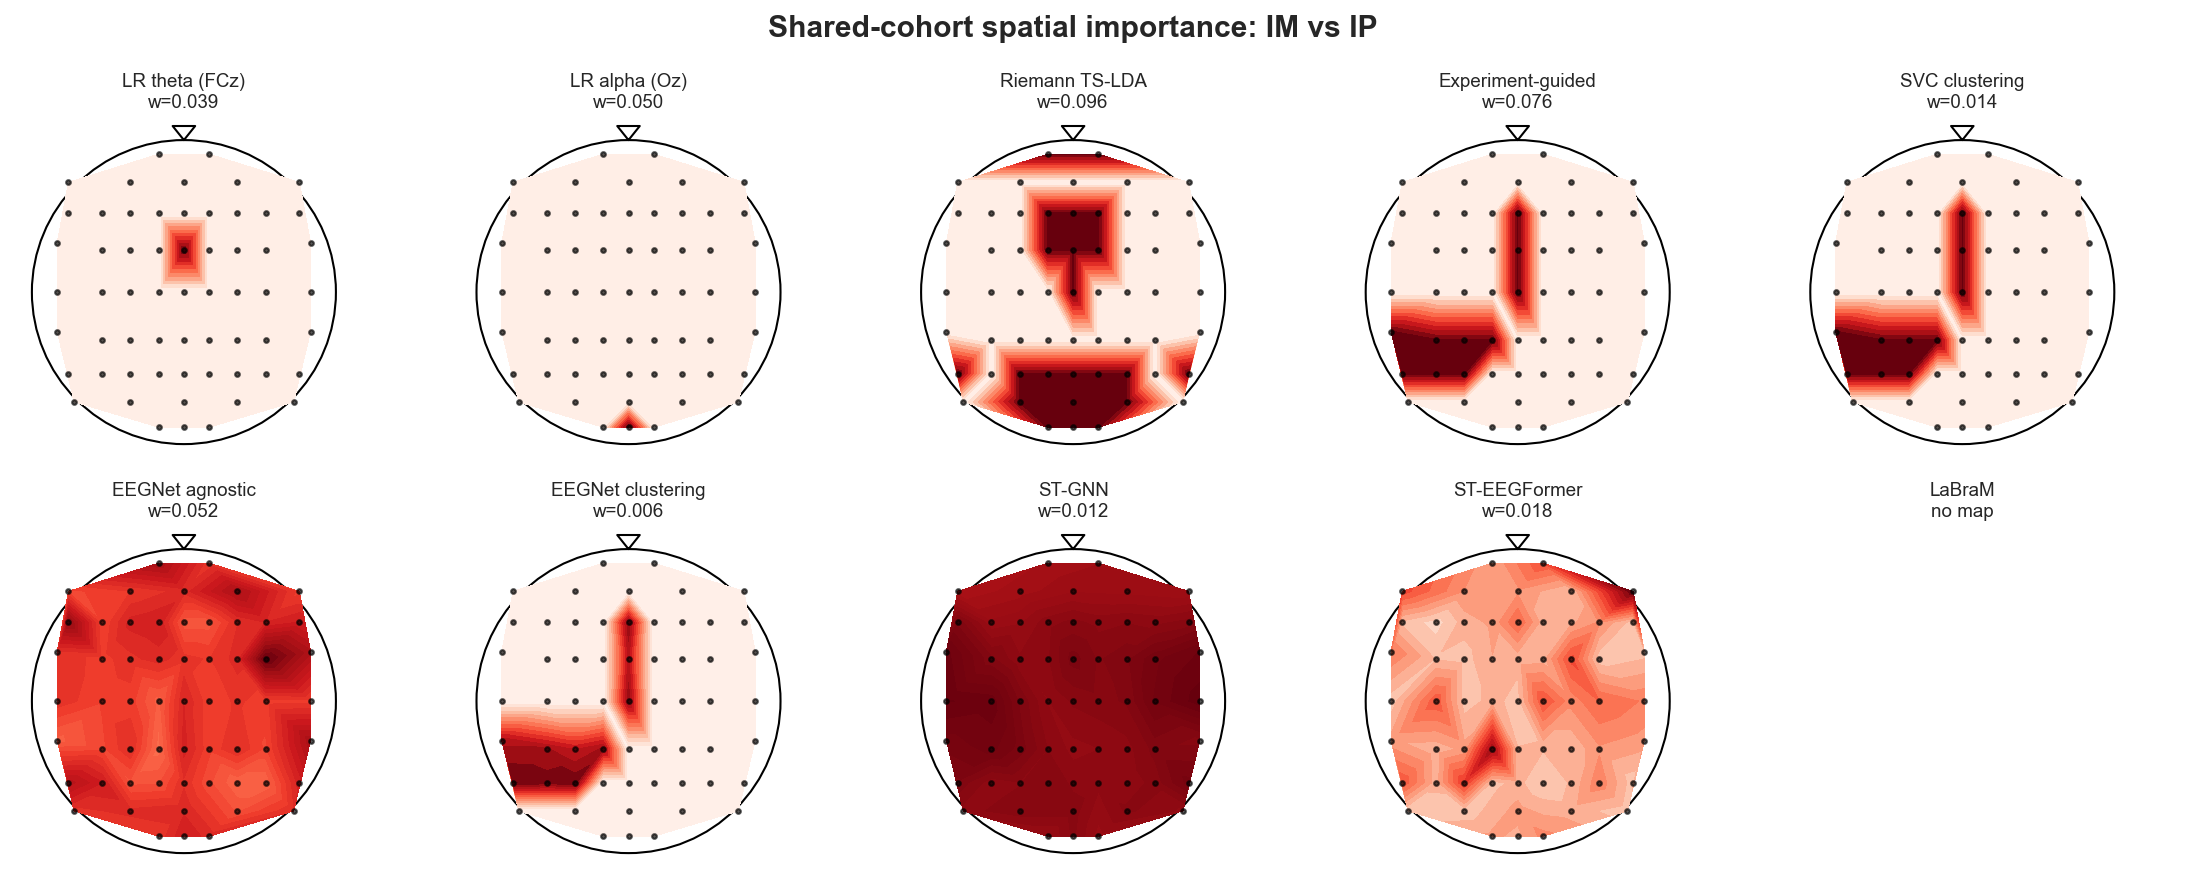
\includegraphics[width=0.96\textwidth]{images/shared_cohort_spatial_topomaps_im_vs_ip.png}
%     \caption{Shared-cohort spatial attribution for IM vs IP. The maps are interpreted cautiously because the corresponding classification performance is close to chance for most model families.}
%     \label{fig:attr-spatial-imip}
% \end{figure}

% In IM vs IP, the spatial maps are therefore framed as a diagnostic of model behaviour rather than a positive result. They help check whether the model is using plausible channels, but the benchmark does not justify a strong physiological claim.

% \begin{figure}[H]
%     \centering
%     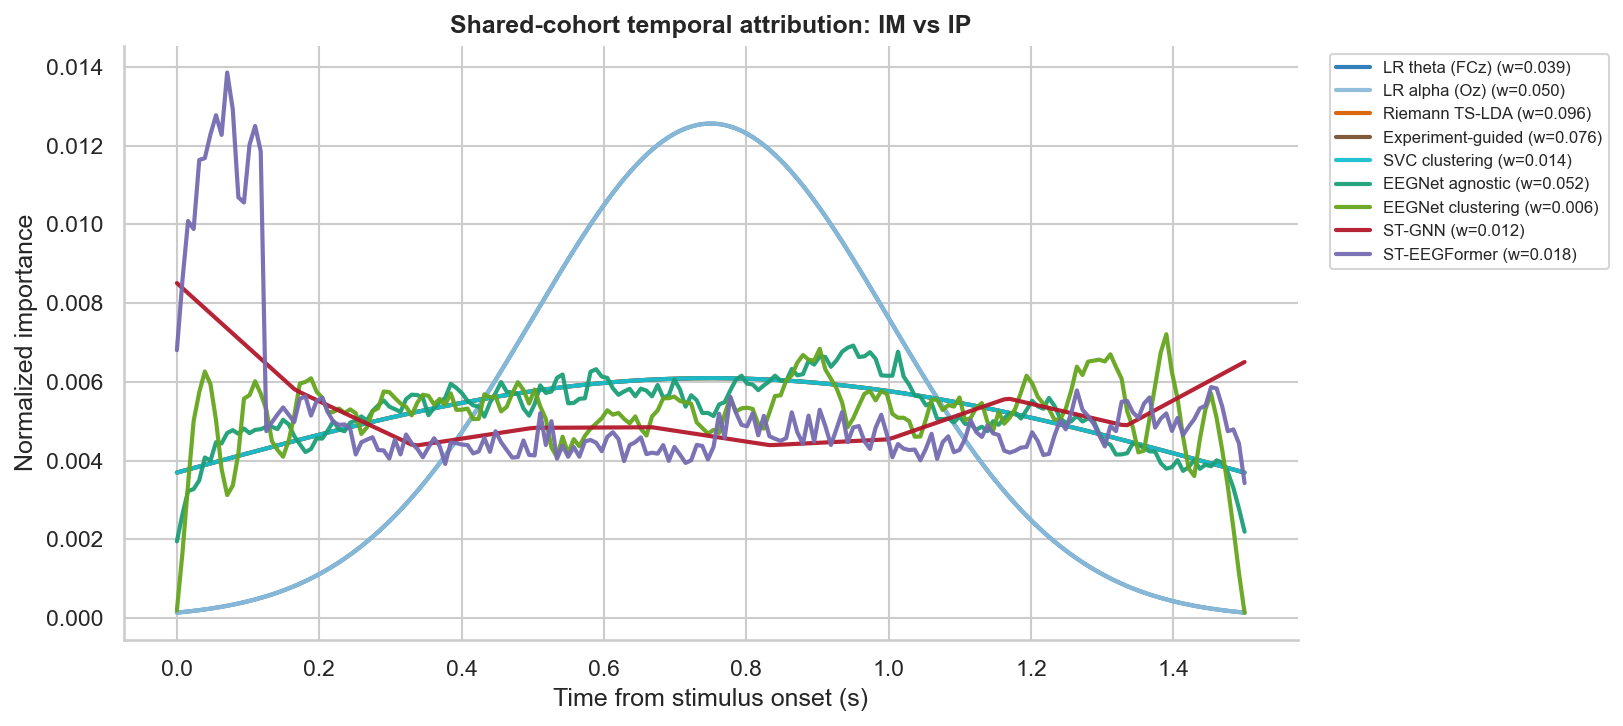
\includegraphics[width=0.90\textwidth]{images/shared_cohort_temporal_attribution_im_vs_ip.png}
%     \caption{Shared-cohort temporal attribution for IM vs IP. The relevance curves are more diffuse than in C vs IP, matching the weaker mixed-versus-pure decoding result.}
%     \label{fig:attr-temporal-imip}
% \end{figure}

% The temporal curves make the same point: some models show peaks, but the agreement is weaker and less clearly tied to the task-level result than in C vs IP.

% \begin{figure}[H]
%     \centering
%     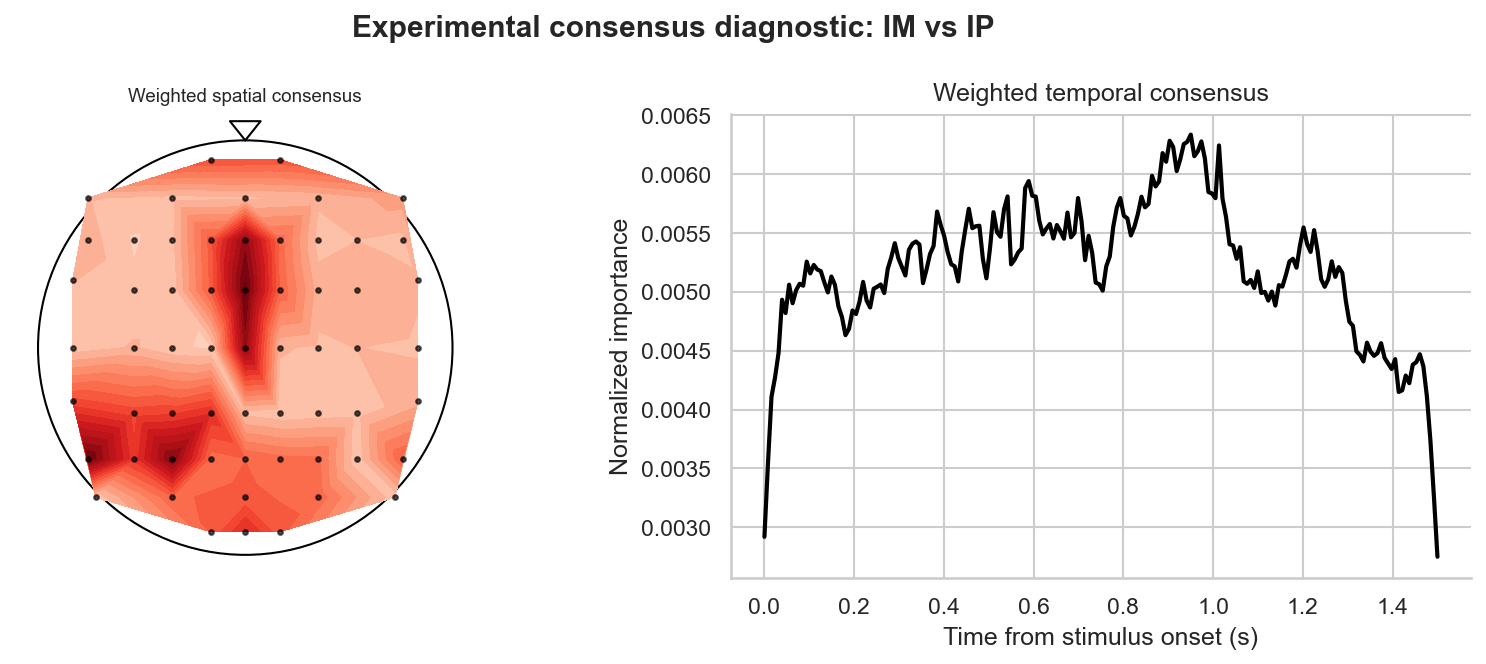
\includegraphics[width=0.90\textwidth]{images/experimental_consensus_diagnostic_im_vs_ip.png}
%     \caption{Consensus diagnostic for IM vs IP. The spatial and temporal summaries are useful for model auditing, but they remain exploratory because the task-level evidence is weaker.}
%     \label{fig:attr-consensus-imip}
% \end{figure}
% \begin{figure}[H]
%     \centering
%     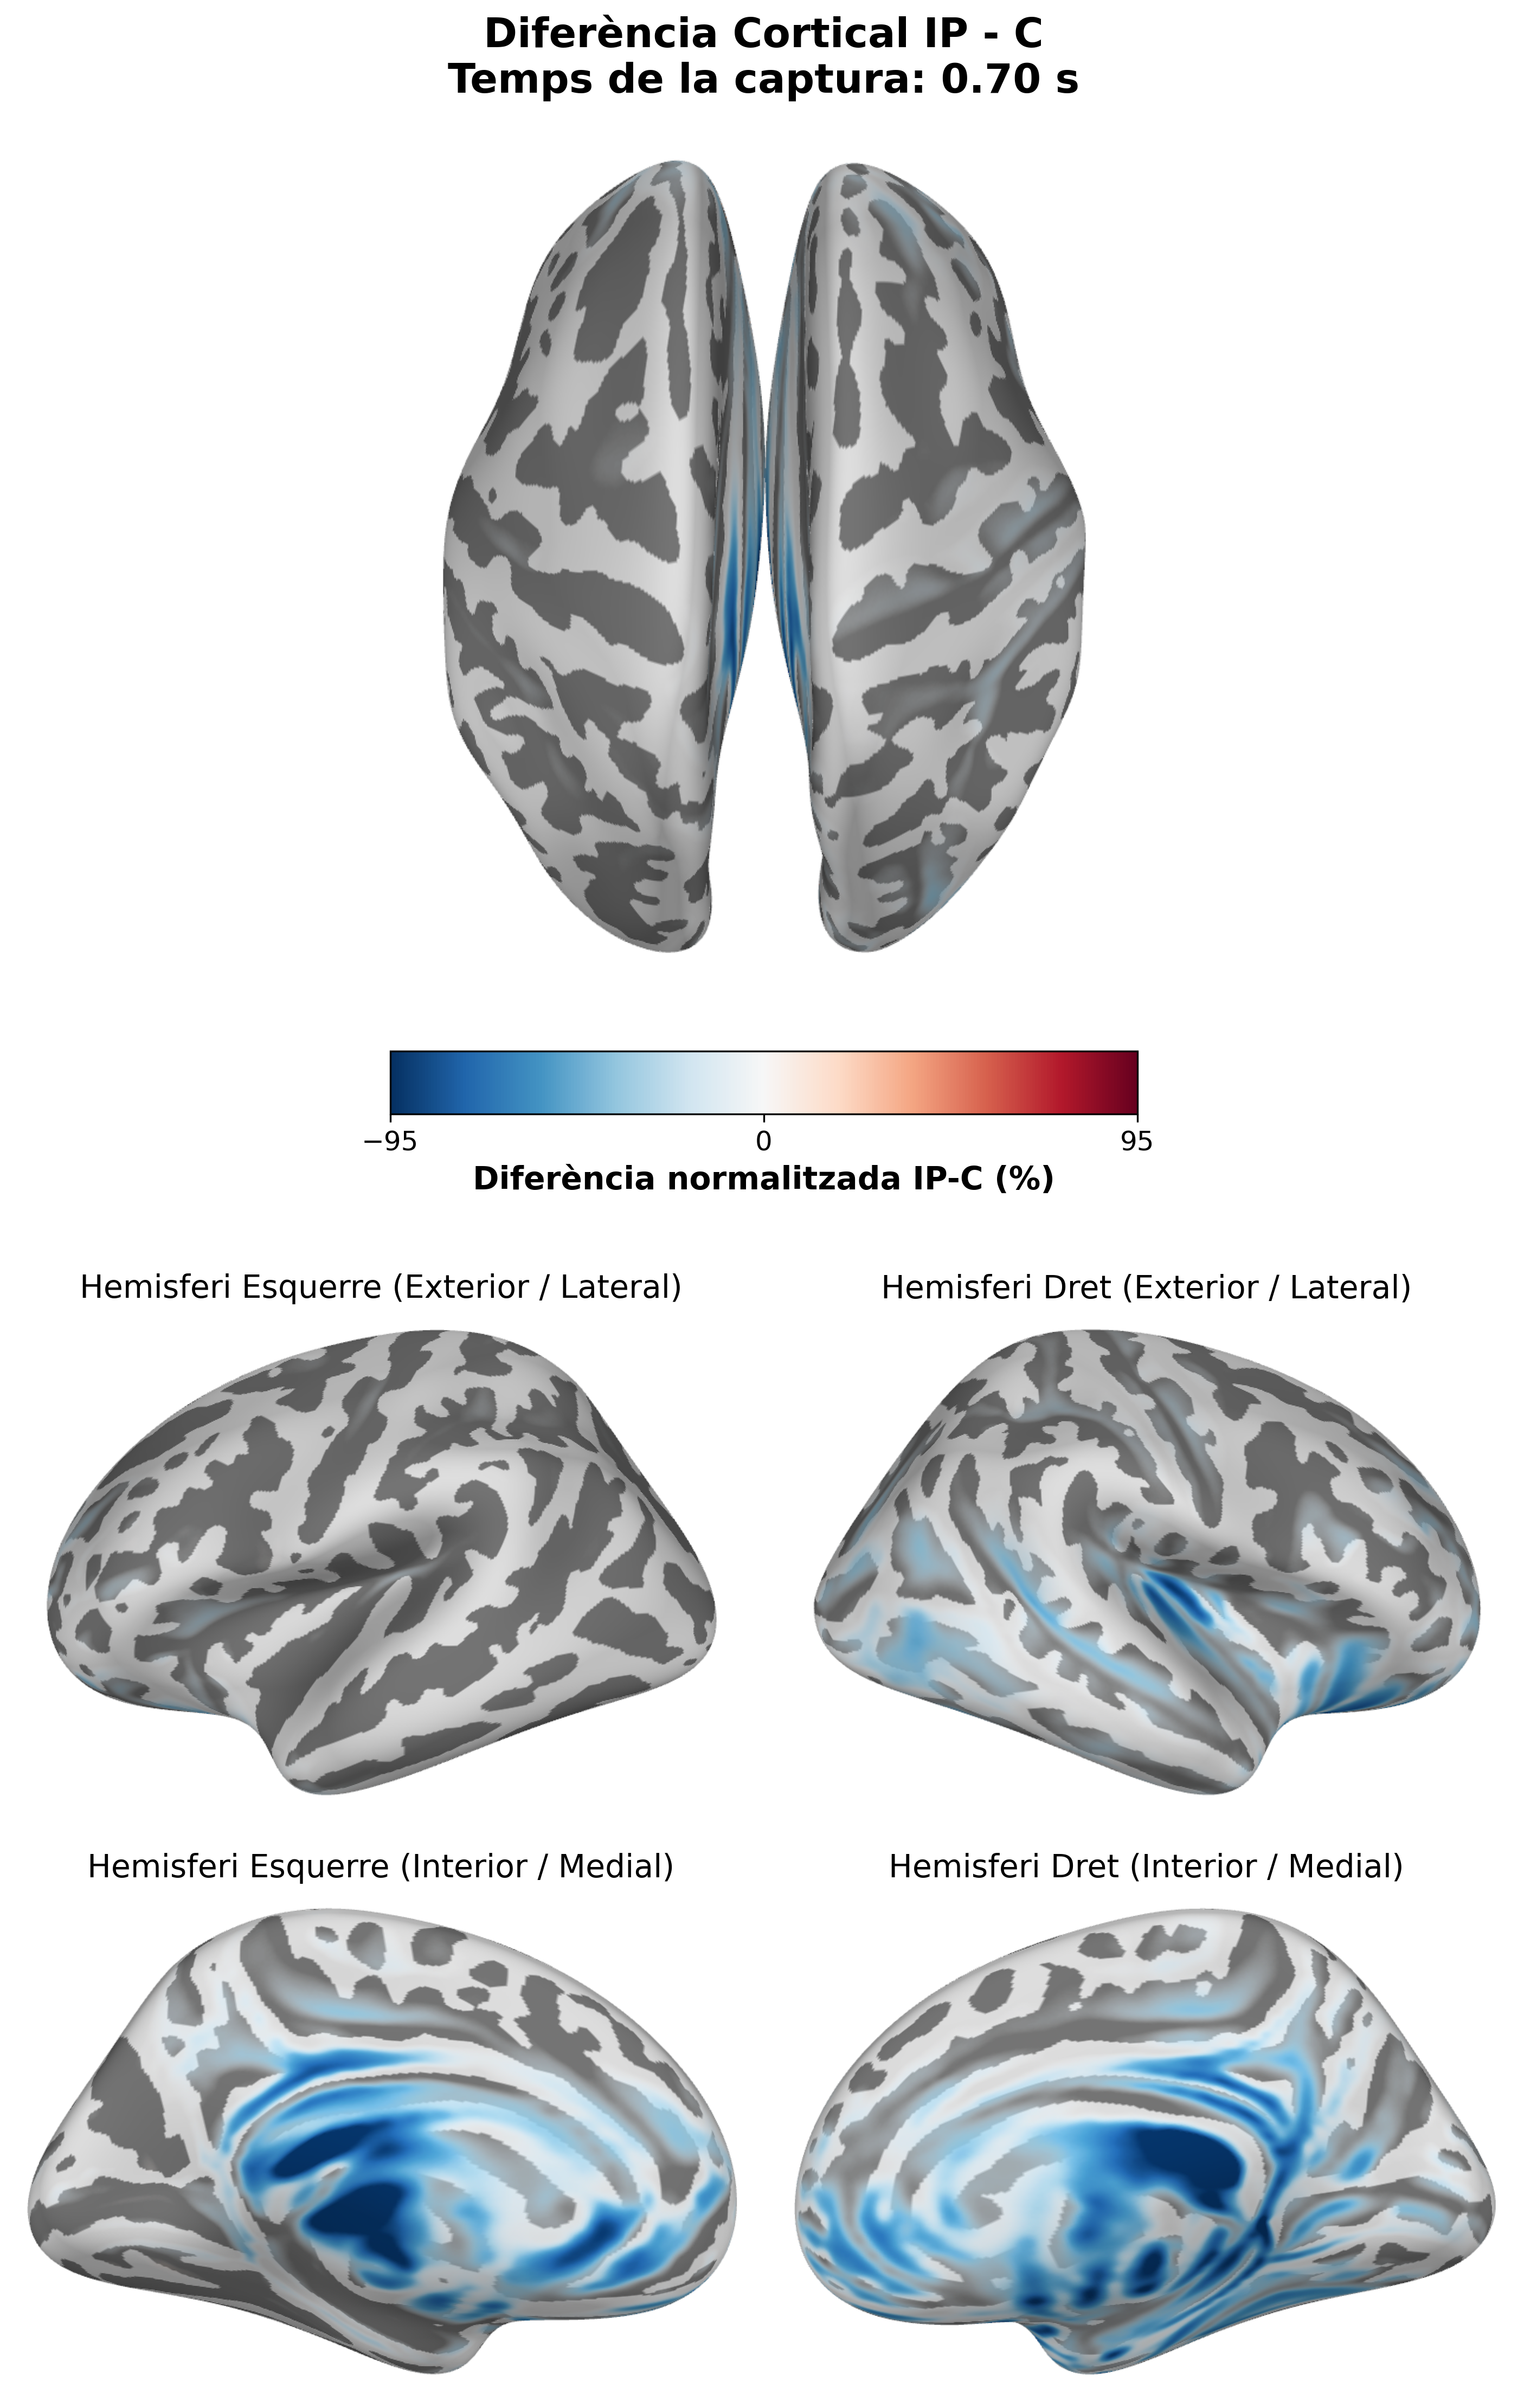
\includegraphics[height=0.76\textheight]{images/3d_master_panel_P057_IP_minus_C_0.70.png}
%     \caption{Example cortical projection for participant P057 at 0.70 s, shown as a qualitative IP--C interpretability view. Because the main thesis claims are sensor-level, this figure is used only as an illustrative bridge between scalp maps and possible cortical distributions.}
%     \label{fig:cortical-projection-example}
% \end{figure}
% \chapter{Decoding Results}
% \label{chap:results}

% \section{Task-level decoding patterns}

% \atc{As summarized in Table \ref{tab:balanced-accuracy}, the decoding analyses showed a clear difference between the two classification tasks. C vs IP was the more reliable contrast, whereas IM vs IP remained close to chance for most models. This distinction is important because the two tasks do not test the same type of information. C vs IP compares congruent trials with incongruent trials leading to a pure percept, and therefore provides the cleaner test of interocular conflict. IM vs IP compares mixed and pure perceptual outcomes within incongruent stimulation, making it a more subtle and exploratory contrast.}

% \atc{The absolute decoding accuracies were modest. This is expected for single-trial scalp EEG in a subtle perceptual task, and the results should not be interpreted as strong individual-trial prediction. Instead, the relevant question is whether performance is consistently above chance under conservative validation and whether the strongest models point to physiologically plausible representations. Under this interpretation, the C vs IP results provide evidence for weak but structured discriminative information.}

% \atc{For C vs IP, the strongest performance was obtained with Riemannian covariance features combined with LDA. This suggests that the useful information is not fully captured by a single frontal theta or occipital alpha feature, but is better represented as distributed multichannel structure. The experiment-guided classical model and the cluster-restricted SVC also performed above the simplest single-feature baselines, supporting the view that representation choice is central to the decoding result.}

% \atc{For IM vs IP, most models remained close to chance. The best value was obtained with the cluster-restricted SVC, but the margin over other models was small. This should therefore be interpreted as evidence that IM vs IP is unstable in the present dataset, rather than as strong evidence for one specific classifier. This weaker result is scientifically plausible: both IM and IP trials involve incongruent stimulation, and the distinction depends on the subjective perceptual report rather than on a clean physical stimulus difference.}

% \atc{Thus, the contrast between C vs IP and IM vs IP is one of the main findings of the decoding analysis. C vs IP provides limited but interpretable evidence for conflict-related EEG information, whereas IM vs IP remains exploratory.}

% \section{Model comparison}

% \atc{Table~\ref{tab:balanced-accuracy} summarises the final balanced-accuracy comparison. The main result is that increasing model complexity did not systematically improve decoding. Classical and Riemannian approaches performed at least as well as, and in some cases better than, compact neural networks and pretrained foundation-model adaptations. This suggests that the limiting factor is not simply classifier expressivity, but the combination of signal-to-noise ratio, subject variability, feature representation, and validation constraints.}

% \begin{table}[H]
%     \centering
%     \caption{Reserved final-holdout balanced accuracy summary.}
%     \label{tab:balanced-accuracy}
%     \small
%     \begin{tabularx}{\textwidth}{@{}lcc@{}}
%         \toprule
%         Model                          & C vs IP Balanced Accuracy (\%) & IM vs IP Balanced Accuracy (\%) \\
%         \midrule
%         Logistic regression, FCz-theta & 49.6 $\pm$ 6.7                 & 50.6 $\pm$ 8.6                  \\
%         Logistic regression, Oz-alpha  & 53.6 $\pm$ 8.2                 & 49.4 $\pm$ 8.0                  \\
%         Riemannian covariance + LDA    & \textbf{58.7 $\pm$ 8.3}        & 49.3 $\pm$ 6.1                  \\
%         Experiment-guided classical ML & 56.9 $\pm$ 8.1                 & 50.9 $\pm$ 8.1                  \\
%         SVC cluster features           & 56.2 $\pm$ 6.3                 & \textbf{52.7 $\pm$ 6.2}         \\
%         EEGNet agnostic                & 53.2 $\pm$ 8.2                 & 49.5 $\pm$ 5.8                  \\
%         EEGNet clustering              & 49.6 $\pm$ 8.0                 & 48.5 $\pm$ 7.5                  \\
%         ST-GNN                         & 52.0 $\pm$ 7.3                 & 51.4 $\pm$ 5.6                  \\
%         ST-EEGFormer                   & 52.5 $\pm$ 8.3                 & 50.7 $\pm$ 5.8                  \\
%         LaBraM adaptation              & 51.9 $\pm$ 6.8                 & 48.2 $\pm$ 9.6                  \\
%         \bottomrule
%     \end{tabularx}
% \end{table}


% \atc{For C vs IP, the best model was Riemannian covariance + LDA, reaching $58.7\%$ balanced accuracy. This was followed by the experiment-guided classical model and the SVC trained on cluster-derived features. For IM vs IP, the best value was obtained with the cluster-restricted SVC, but the absolute performance remained low at $52.7\%$. The difference between the two contrasts supports the interpretation that C vs IP contains more stable discriminative information than IM vs IP.}

% \atc{The deep-learning models did not clearly outperform the classical baselines. EEGNet, ST-GNN, ST-EEGFormer and LaBraM remained close to chance or only modestly above it. Therefore, these models should be treated as exploratory comparisons rather than as central evidence. Their weak performance is nevertheless informative, because it shows that larger or more flexible models do not automatically improve decoding in this dataset.}

% \atc{The cluster-restricted SVC result should also be interpreted cautiously. If the clusters used to define the features were selected using the full dataset, the decoding estimate may be optimistic because the same data contributed to feature selection and performance evaluation. A confirmatory version of this analysis would require cluster selection inside each training fold, or clusters defined from an independent dataset or previous study.}

% \atc{The previously reported observation that the best-performing subjects reached higher accuracies should be treated as exploratory only. Unless these subjects were selected using an independent criterion defined before decoding, this type of subgroup analysis can overestimate the apparent strength of the effect. It may be mentioned as evidence of inter-subject variability, but it should not be used as a main result.}

% \begin{figure}[H]
% \centering
% \panelimage{0.8\textwidth}{images/cohort_roc_pr_curves_c_vs_ip.png}{C vs IP cohort ROC and precision--recall curves.}
% \hfill
% \panelimage{0.86\textwidth}{images/cohort_roc_pr_curves_im_vs_ip_comparison.png}{IM vs IP cohort ROC and precision--recall curves.}
% \caption{\atc{Cohort-level discrimination curves for the two binary tasks. C vs IP shows the clearer above-chance pattern, led by Riemannian covariance, whereas IM vs IP remains close to chance for most models.}}
% \label{fig:cohort-roc-pr-curves}
% \end{figure}

% \atc{The ROC and precision--recall curves support the same task-level interpretation as Table~\ref{tab:balanced-accuracy}. The C vs IP curves show a more consistent separation between models, whereas the IM vs IP curves remain clustered near chance. Thus, the curve-level evidence reinforces the conclusion that C vs IP is the more reliable decoding task.}

% \section{Pipeline and configuration effects}

% \atc{The configuration analyses indicate that decoding performance depends on the complete analysis pipeline, not only on the final classifier. Choices such as frequency band, time window, channel set, scaling strategy, covariance representation, and model family can all influence performance. This is particularly important in low-SNR EEG, where small preprocessing choices may determine whether a weak effect is preserved or removed.}

% \atc{For C vs IP, the best-performing configuration favoured distributed covariance-based decoding, consistent with the idea that the relevant information is spatially distributed rather than restricted to a single electrode. For IM vs IP, the best-performing configuration was more constrained and alpha/ROI-based, but the overall decoding performance remained weak. This reinforces the interpretation that IM vs IP is exploratory.}

% \begin{figure}[H]
% \centering
% \panelimage{0.8\textwidth}{images/experiment8_marginal_component_means.png}{Marginal accuracy by component value.}
% \hfill
% \panelimage{0.39\textwidth}{images/experiment10_component_contributions.png}{One-at-a-time component contributions.}
% \caption{\atc{Configuration-search summaries. The results indicate that preprocessing, spatial scope, spectral representation, temporal window, and classifier family jointly shape decoding performance.}}
% \label{fig:configuration-search-summaries}
% \end{figure}

% \atc{Figure~\ref{fig:configuration-search-summaries} should be interpreted as a methodological diagnostic rather than as an independent confirmatory result. It shows that model family cannot be evaluated separately from the representation provided to the model. However, if many configurations were searched on the same dataset, the selected configuration may be optimistic unless it was evaluated using a nested procedure or an independent holdout set.}

% \section{Interpretability}

% \atc{The interpretability analyses were used as diagnostics of model behaviour, not as independent evidence for neural mechanisms. Their purpose was to check whether models with above-chance performance relied on channels and time windows compatible with the theta/alpha effects observed in the previous analyses. A visually structured attribution map from a near-chance model should not be interpreted as physiological evidence.}

% \atc{For C vs IP, attribution is potentially informative because the decoding benchmark provides some evidence for above-chance classification, especially for the classical and Riemannian models. The relevant question is whether model-relevant sensors and time windows are compatible with the posterior alpha and fronto-medial theta patterns observed in the statistical analyses.}

% \begin{figure}[H]
% \centering
% 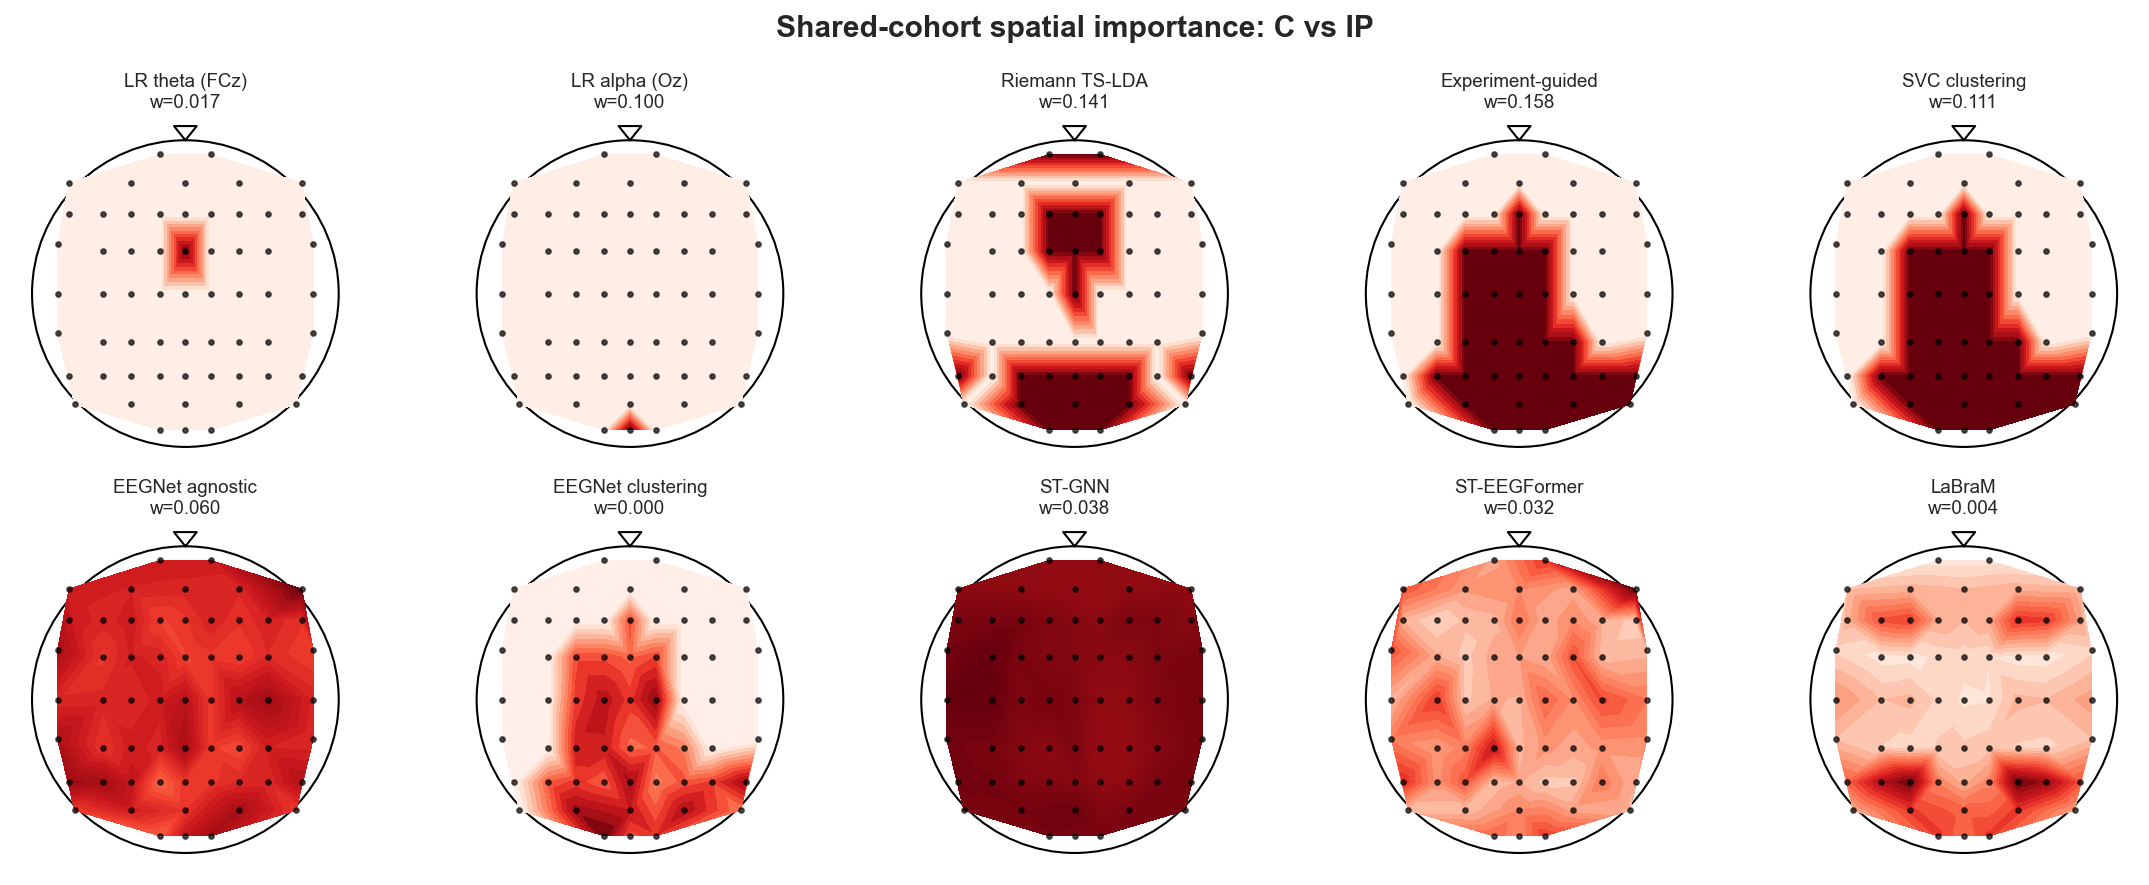
\includegraphics[width=0.96\textwidth]{images/shared_cohort_spatial_topomaps_c_vs_ip.png}
% \caption{\atc{Shared-cohort spatial attribution for C vs IP. The maps are interpreted as sensor-level diagnostics of model behaviour, not as source-localisation results.}}
% \label{fig:attr-spatial-cvip}
% \end{figure}

% \atc{The C vs IP attribution maps should be read together with the decoding results and the cluster-based analyses. Their value is not that they provide an independent proof of a neural source, but that they help assess whether the models rely on plausible sensor-level information. Heterogeneous or diffuse maps from weak models should be interpreted cautiously.}

% \atc{For IM vs IP, attribution results should remain exploratory and can be moved to the appendix. Since most IM vs IP models perform close to chance, the corresponding attribution maps are better understood as model-auditing outputs than as evidence for a reliable EEG signature of mixed versus pure perceptual reports.}

% \atc{The cortical projection figure should also be moved to the appendix or removed from the main thesis. Because the main analyses are sensor-level scalp EEG analyses, a cortical projection may give the misleading impression that the thesis makes a source-level claim. If retained, it should be explicitly labelled as a qualitative illustration rather than as evidence for cortical localisation.}

\chapter{Discussion}
\label{chap:discussion}

\section{Scientific Interpretation of the Two Contrasts}
The replication results give a partial but useful agreement with the original paper. The clearest overlap is the alpha-related C vs IP effect, which appears in posterior sensors over a broad post-stimulus interval. The theta story is more delicate: fronto-medial theta remains theoretically relevant and appears in small late clusters, but it is not strong as a simple single-channel scalar feature. This does not invalidate the conflict-monitoring account. It shows that the expression of conflict-related information in scalp EEG depends on the representation used to measure it.

C vs IP is the central scientific result because both conditions produce pure reports, while only IP contains interocular conflict. Above-chance decoding in this contrast therefore suggests that the EEG contains information related to the presence of conflict, not merely to whether a participant pressed a different button or reported a mixed percept. The strongest interpretation is cautious: the signal is weak but structured. It is not a clean neural readout of conscious content, but neither is it random noise. Posterior alpha, distributed covariance, and the C vs IP cluster maps together suggest that conflict-related perceptual information is present in the sensor-level EEG.

The safest reading is not that posterior alpha replaces fronto-medial theta. A better interpretation is that the original theory points to relevant physiological processes, while the most decodable implementation in this dataset is distributed. Single-channel theta is too narrow a view of the signal; posterior alpha is more stable as a scalar feature; and covariance models capture relationships that neither scalar baseline can see. This is a common situation in EEG: the theoretical label may be local or frequency-specific, but the measurable scalp signature is broader because of source mixing, subject variability, and preprocessing choices.

IM vs IP is a harder and less settled contrast. Both classes are incongruent, so the difference is not conflict versus no conflict but mixed versus pure perceptual outcome under conflict. The mixed label may also be heterogeneous. One participant's mixed percept may be a spatial patchwork of red and green, another's may be unstable over the stimulus interval, and another's may reflect uncertainty at report. These are behaviorally similar enough to share a label, but they may not correspond to one compact EEG signature. Trial-count limitations and time-window mismatch can further weaken the contrast. For that reason, IM vs IP should be presented as an exploratory result rather than as the main evidence for perceptual decoding.

\section{Why the Best Models Are Not the Largest Models}
Riemannian covariance decoding performs best for C vs IP because its inductive bias matches the data. EEG has low signal-to-noise ratio, strong spatial mixing, and relatively few trials after subject-wise balancing. A covariance matrix preserves distributed relationships between channels while keeping the number of trainable parameters small. OAS shrinkage stabilizes the covariance estimate, tangent-space projection makes the representation usable for a linear classifier, and shrinkage LDA keeps the final decision rule simple. This is a good match for a dataset where the discriminative effect is likely broad, weak, and subject-dependent. For IM vs IP, the final-holdout ranking is flatter and led by the cluster-restricted SVC, which reinforces the view that this contrast is less stable.

This helps explain why deep learning does not dominate. EEGNet remains a useful neural baseline because it was designed for EEG and imposes temporal and spatial filtering structure. However, larger models do not automatically improve the result. The dataset is small, subject variability is high, labels are imbalanced before correction, and the effect of interest is subtle. A flexible model can spend capacity on noise structure, session structure, or preprocessing artefacts instead of the perceptual contrast of interest. More capacity is useful only when the training data and validation design support it.

The fact that the larger models do not win should be treated as a result, not merely as a failed attempt. It shows that the limiting factor is not only architecture. Under realistic EEG constraints, the most effective choices are often those with the strongest inductive bias: covariance geometry for distributed low-SNR signals, compact EEG-specific convolutions for learned temporal-spatial filters, and narrow feature baselines for hypothesis checking. A deep model that is more expressive but less well matched to the dataset can be worse than a simpler model that preserves the relevant structure.

The difference between agnostic EEGNet and cluster-restricted EEGNet illustrates this point. The cluster-restricted variant is biologically motivated because it focuses on theta/alpha windows selected by the clustering analysis. However, this restriction can also remove useful context. The agnostic model sees all 60 channels and the full broadband analysis window, so it can learn auxiliary spatial and temporal patterns that are not included in the exported clusters. It also avoids depending too strongly on a cluster-selection step that may be unstable across subjects, especially for IM vs IP. In this dataset, the agnostic variant therefore appears more robust: it is less constrained by an imperfect prior, while still being compact enough not to behave like a large unrestricted deep model.

The foundation-model results should be interpreted even more carefully. Underperformance by ST-EEGFormer or LaBraM-style adaptation in this thesis is not evidence that EEG foundation models are generally ineffective. It may reflect domain gap, checkpoint mismatch, channel-layout differences, resampling constraints, patch format, LoRA settings, or simply the limited downstream dataset. The useful conclusion is narrower and more practical: pretrained models do not remove the need for careful data representation, channel mapping, validation, and task-specific calibration.

\section{Limitations}
The modeling results show that EEG decoding is a pipeline problem. Filtering, time window, channel selection, normalization, representation, model family, balancing strategy, and validation split all interact. A model can only learn what the representation preserves. Trial-wise z-scoring changes whether absolute amplitude differences are available; band-pass filtering decides which frequency structure survives; ROI selection can remove noise but also discard distributed signal; and fold design determines whether performance reflects the condition or leakage from subject/session structure.

However, this does not mean that the model selected does not matter, but that without a good representation, complex model architectures that try to do too much can perform worse than simpler solutions. Because the accuracies are modest, accuracy alone is not enough to support the thesis argument. The strongest case combines performance, permutation testing, spatial maps, temporal windows, spectral interpretation, Jaccard cluster variability, and cross-model convergence. Attribution plots are useful only under those constraints. A visually plausible attribution map is weak evidence if the model is near chance, if the cache is incomplete, or if the highlighted region disagrees with independent cluster evidence. Conversely, modest accuracy becomes more meaningful when the model's relevant channels and windows align with posterior alpha, fronto-medial theta, and the permutation clusters.

The limitations follow directly from this pipeline view. The accuracies are modest, so the thesis must avoid strong claims about mental-state reading. Subject variability is large, so cohort averages should be accompanied by subject-level distributions and selection tables. The IM vs IP margins are small, so changes in preprocessing, windowing, or final cache regeneration could alter the ranking even if the overall near-chance conclusion remains. Cluster-guided decoding carries circularity risk, so cluster selection and final evaluation must be separated conceptually and, where possible, procedurally. Finally, all topographic language remains sensor-level unless source localisation is performed. These limitations do not make the project weak; they define the boundary of what a careful EEG decoding thesis can responsibly claim.

\chapter{Ethics}
\label{chap:ethics}

\section{Privacy}
To establish the ethical and methodological boundaries of EEG decoding, this thesis includes a subject-identity control task. Instead of predicting the perceptual condition, the control asks whether a model can identify which participant produced a held-out EEG epoch.

The available subject-identity control identifies participants with more than 98\% accuracy on average. This is in line with results from the literature~\cite{jijomon_person-identification_2021} and confirms that the recordings contain stable person-specific structure. Methodologically, it explains why random trial splits are dangerous in EEG: a model can learn identity, session structure, or subject-specific response tendencies instead of the condition of interest. It also explains why inter-subject models have to actively deter models from predicting which subject it is, since most of the variance of an EEG is unique to the person. Ethically, it means that EEG should be treated as biometric data even after ordinary metadata anonymization.

High subject-identification accuracy also raises privacy concerns. If de-identified raw EEG recordings were linked to a reference database from the same people, re-identification could become possible. This vulnerability means that sharing raw EEG data requires strict ethical oversight, secure repository platforms, access-control agreements, and explicit participant consent regarding the sharing of neural biometric data.

Responsible storage and sharing of EEG recordings require anonymization, access control, and respect for the consent conditions under which the original data were collected. The original data collection should be described in relation to ethical approval and informed consent as reported by the source study. This thesis relies on secondary analysis of those recordings, so it does not introduce new participant risk through data collection, but it still has a responsibility to handle the recordings, caches, and subject-level outputs carefully.

\section{Open Science}
In the spirit of transparency, all the Jupyter notebooks and python code have been made publicly available on github~\cite{noauthor_nilsdurantfg_nodate}. The data was already public from the original article~\cite{torralba_cuello_evaluating_2025, drew_binocular_2026}.

\chapter{Conclusions}
\label{chap:conclusions}

\section{Answers to the Objectives}
The project replicates part of the original theta/alpha story, extends the analysis to channel-by-time clustering, evaluates a broad model suite, and interprets results through validation and attribution diagnostics. C vs IP shows weak but structured decoding. IM vs IP remains exploratory.

The first objective was replication. The thesis finds partial agreement with the original paper: posterior alpha effects in C vs IP are the most robust overlap, while theta effects are more fragile and depend more strongly on representation and window choice.

The second objective was the 2D extension. The spatiotemporal clustering analysis identifies channel-time clusters and, through Jaccard divergence, shows that cluster stability differs across contrasts and bands. C vs IP alpha is the most reproducible cluster, while IM vs IP clusters are less stable.

The third objective was decoding. The answer is cautiously positive for C vs IP and much weaker for IM vs IP. Riemannian covariance plus LDA is the strongest current model family, suggesting that distributed covariance captures information missed by isolated scalar power features.

The final objective was to interpret the results of the decoding. The results imply that decoding on a single electrode isn't as strong as using a combination of electrodes and time-steps. And different models use very different combinations of electrodes and times. Some give more or less equal importance to all electrodes, while others specialize in certain regions (parieto-occipital, frontal). The temporal attribution has less consensus than the spatial

\section{Takeaways}
The scientific takeaway is that conflict-related perceptual information is present in the EEG, but it is subtle, distributed, and validation-sensitive. The result supports cautious condition decoding rather than strong claims about conscious-state inference. Binocular rivalry remains a useful tool because it separates physical stimulation, perceptual outcome, and report more cleanly than many perceptual paradigms, but EEG does not provide a direct window into conscious content.

The methodological takeaway is that classical methods with strong EEG-specific inductive biases can outperform or match complex models under realistic constraints. Riemannian covariance decoding is the clearest example. This does not mean deep learning is inappropriate for EEG; it means that deep learning requires enough data, compatible representations, careful validation, and a well-matched architecture. In this project, preprocessing and representation choices matter as much as model family.

\section{Future Work}
Future work should first strengthen the empirical base of the project. More subjects and trials would make the C vs IP result more reliable and would give the harder IM vs IP contrast a fairer test. A larger dataset would also allow stricter cross-subject generalization, where models are evaluated on participants that were never seen during training. This would make it easier to distinguish genuinely condition-related EEG structure from subject-specific signatures, session drift, or preprocessing artifacts.

A second direction is to improve the neurophysiological interpretation. The present thesis remains deliberately sensor-level: topographies show where effects appear on the scalp, not where they originate in the brain. Future work could add source localization, better individual head models, and more systematic comparison between posterior alpha, fronto-medial theta, and distributed covariance patterns. This would help test whether the model-relevant features align with plausible neural generators or mainly reflect sensor-level mixtures.

The modeling pipeline also leaves clear technical next steps. The Foundation-model adaptation should be tuned more carefully, including channel mapping, patching strategy, LoRA settings, and the match between pretraining data and the binocular-rivalry task. These models should be treated as hypotheses about transferable EEG structure, not as automatic performance upgrades.

Finally, a stronger future version of the project would separate exploratory cluster discovery from confirmatory decoding more sharply. The final time windows, frequency bands, and ROIs could be pre-registered after an exploratory phase, then tested on held-out subjects or a separate dataset. It would also be useful to evaluate subject-specific calibration: calibration may improve decoding, but it should be measured against the loss of generality in the scientific claim.

\begin{appendices}

    \chapter{Abbreviations}
    \markboth{Abbreviations}{Abbreviations}
    \label{app:abbreviations}
    These are the main abbreviations used throughout the thesis. The condition labels are analysis labels assigned after combining the stimulus configuration with the participant's red, green, or mixed report.


    \begin{longtable}{p{0.18\linewidth}p{0.74\linewidth}}
        \toprule
        Term & Meaning                                                                                                           \\
        \midrule
        EEG  & Electroencephalography, scalp voltage measurements reflecting synchronized neural population activity.            \\
        BR   & Binocular rivalry, the perceptual competition that occurs when incompatible images are presented to the two eyes. \\
        C    & Congruent condition: both eyes receive compatible input and the participant reports a pure percept.               \\
        IP   & Incongruent Pure condition: eyes receive incompatible input and the participant reports a pure percept.           \\
        IM   & Incongruent Mixed condition: eyes receive incompatible input and the participant reports a mixed percept.         \\
        ROI  & Region of interest, here used for sensor groups rather than anatomical source regions.                            \\
        CV   & Cross-validation, the procedure for estimating generalisation on held-out folds.                                  \\
        OAS  & Oracle Approximating Shrinkage, a covariance shrinkage estimator.                                                 \\
        LDA  & Linear Discriminant Analysis.                                                                                     \\
        SVC  & Support Vector Classifier.                                                                                        \\
        LoRA & Low-Rank Adaptation, a parameter-efficient fine-tuning method.                                                    \\
        ROC  & Receiver Operating Characteristic.                                                                                \\
        AUC  & Area Under the Curve.                                                                                             \\
        \bottomrule
    \end{longtable}

    \chapter{Work Plan}
    \label{app:work-plan}
    The project was planned as a 20-week TFG, with an additional week 0 reserved for the initial meeting and project framing. The expected effort follows the standard FIB workload estimate of 30 hours per ECTS credit. Since the thesis has 18 ECTS, the planned workload is therefore
    \[
        18 \times 30 = 540 \text{ hours}.
    \]
    The first four weeks were intentionally lighter in implementation work because they coincided with the end of the Erasmus period. During that interval, the project was limited to environment setup, access to the dataset, and literature review. Coding, experimentation, clustering, and model training started after this initial phase.

    \textbf{Timeline}
    Figure~\ref{fig:gantt-work-plan} summarizes the final plan. Meetings are represented with diamonds, while assessed deliveries are represented with square markers and staggered labels. This distinction matters because weeks 17 and 19 contain both a meeting and a delivery, but they are not the same event.

    \begin{figure}[H]
        \centering
        \resizebox{\textwidth}{!}{%
            \begin{tikzpicture}[
                    x=0.50cm,
                    y=0.62cm,
                    task/.style={draw=black!45, rounded corners=1pt, minimum height=0.35cm},
                    meeting/.style={diamond, draw=blue!65!black, fill=blue!18, inner sep=1.6pt},
                    delivery/.style={draw=red!65!black, fill=red!18, minimum width=0.30cm, minimum height=0.30cm},
                    font=\scriptsize
                ]
                \foreach \w in {0,...,20} {
                        \draw[black!12] (\w,0) -- (\w,-11.0);
                        \node[anchor=south] at (\w+0.5,0.1) {\w};
                    }
                \node[anchor=east, font=\scriptsize\bfseries] at (-0.1,0.35) {Week};

                \foreach \y/\label in {
                -0.8/{Setup and data access},
                -1.6/{Literature review},
                -2.4/{Exploration and preprocessing},
                -3.2/{Paper replication},
                -4.0/{2D clustering and Jaccard},
                -4.8/{Classical decoding},
                -5.6/{Deep/foundation models},
                -6.4/{Interpretability and controls},
                -7.2/{Writing and revision},
                -8.0/{Presentation preparation},
                -8.8/{Meetings},
                -9.8/{Deliveries}
                } {
                \node[anchor=east] at (-0.1,\y) {\label};
                }

                \filldraw[task, fill=blue!25]   (1,-1.0) rectangle (4,-0.6);
                \filldraw[task, fill=teal!25]   (1,-1.8) rectangle (5,-1.4);
                \filldraw[task, fill=teal!25]   (9,-1.8) rectangle (12,-1.4);
                \filldraw[task, fill=green!25]  (5,-2.6) rectangle (7,-2.2);
                \filldraw[task, fill=orange!30] (6,-3.4) rectangle (9,-3.0);
                \filldraw[task, fill=purple!20] (8,-4.2) rectangle (12,-3.8);
                \filldraw[task, fill=red!20]    (10,-5.0) rectangle (14,-4.6);
                \filldraw[task, fill=cyan!25]   (12,-5.8) rectangle (17,-5.4);
                \filldraw[task, fill=gray!25]   (14,-6.6) rectangle (18,-6.2);
                \filldraw[task, fill=yellow!35] (5,-7.4) rectangle (19,-7.0);
                \filldraw[task, fill=lime!30]   (19,-8.2) rectangle (20,-7.8);

                \foreach \m in {0,4,6,11,13,14,16,17,19} {
                        \node[meeting] at (\m+0.5,-8.8) {};
                    }
                \node[anchor=north, align=center, font=\tiny] at (0.5,-9.05) {Initial\\meeting};

                \node[delivery] at (17.5,-9.8) {};
                \draw[red!60!black, thin] (17.5,-9.98) -- (16.7,-10.45);
                \node[anchor=north, align=center, font=\tiny] at (16.7,-10.45) {Monitoring\\report};
                \node[delivery] at (19.5,-9.8) {};
                \draw[red!60!black, thin] (19.5,-9.98) -- (19.15,-10.95);
                \node[anchor=north, align=center, font=\tiny] at (19.15,-10.95) {Report\\submission};
                \node[delivery] at (20.5,-9.8) {};
                \draw[red!60!black, thin] (20.5,-9.98) -- (20.85,-10.45);
                \node[anchor=north, align=center, font=\tiny] at (20.85,-10.45) {Presentation};
            \end{tikzpicture}
        }
        \caption{Gantt chart of the 20-week work plan, plus week 0 for the initial meeting. The first four weeks contain only setup and literature review because they overlap with the end of the Erasmus period.}
        \label{fig:gantt-work-plan}
    \end{figure}

    The main technical risks were class imbalance, session drift, circularity in cluster selection, and overfitting to subject-specific EEG structure. These risks shaped the schedule: exploratory analysis and clustering were kept separate from final decoding evaluation, validation used grouped folds where appropriate, and the deep-learning experiments were run after classical baselines had established a lower-cost reference point.

    \chapter{Economic Viability}
    \label{app:cost}
    The economic analysis is approximate because the project is a university thesis rather than a commercial product. The thesis did not require paid software licenses or specialized data acquisition because it reuses an existing EEG dataset and open-source tools.

    \paragraph{Human resources.}
    The dominant cost is the 540 hours of student work implied by the 18 ECTS workload. As a rough reference, valuing this time at 10 EUR/hour, the standard order of magnitude for FIB student internships, gives about 5,400 EUR of student labour. The two advisors are estimated at 50 combined hours. At 30 EUR/hour, this adds about 1,500 EUR. The human-time estimate is therefore roughly 6,900 EUR before considering compute.

    \paragraph{Computing resources.}
    The experiments used approximately 80 hours of NVIDIA T4 GPU time for deep-learning and foundation-model runs, plus about 1,000 hours of local CPU time for preprocessing, feature extraction, cross-validation, clustering, and cached analysis. In practice, the GPU runs were carried out through free Google Colab and Kaggle allocations, so no direct GPU bill was paid by the student. The calculation is still useful as an economic footprint estimate. The CPU work was often parallelized or multi-threaded, so wall-clock time and processor-hour accounting are not identical. The NVIDIA T4 has a 70 W board-power specification, but the estimate below uses 250 W for a full GPU job including the host machine, storage, and cooling overhead \citep{nvidia_t4_product_brief}. It also uses rounded assumptions of 80 W for local CPU computation, 0.20 EUR/kWh for electricity, and 0.20 kgCO$_2$e/kWh for carbon intensity, following the style of simple computational-footprint estimates rather than precise metered billing \citep{lannelongue_green_2021, eurostat_electricity_prices, ember_yearly_electricity_data}. The compute corresponds to
    \[
        80 \times 0.25 + 1000 \times 0.08 = 100 \text{ kWh}.
    \]
    This gives an electricity cost of about 20 EUR and emissions of about 20 kgCO$_2$e. If a T4 GPU is amortized at 1,500 EUR over three years with 30\% effective utilization, the 80 GPU hours add roughly 15 EUR of hardware amortization. The 30\% utilization value is not a measured utilization of Colab or Kaggle infrastructure; it is a conservative accounting assumption for shared academic hardware, included only to avoid pretending that free GPU access has zero economic value. These numbers come from transparent assumptions, not from an electricity bill or cloud invoice. They show that the direct compute cost is modest compared with human time. The project is economically viable because the expensive part is not hardware ownership, but the careful iteration required to make the analysis reliable.

    \chapter{Sustainability Analysis}
    \label{app:sustainability}
    \paragraph{Resource use.}
    The sustainability impact of the project is modest but not negligible. Most of the consumed resources were spent during experimentation: trying preprocessing choices, training model variants, recomputing folds, and checking whether results were stable. This is different from reproducing the final thesis results. Once the final configuration is fixed, the main analyses could be recreated with an estimated 20 GPU hours and 100 CPU hours, a fraction of the original exploratory cost.

    \paragraph{Model choice.}
    The most important sustainability lesson is methodological: a larger neural model is not automatically the most responsible option. In this dataset, classical methods with strong EEG-specific inductive biases are competitive with or better than larger models. Choosing the simplest model that answers the scientific question reduces compute, improves reproducibility, and makes the result easier to audit.

    \paragraph{SDG connection.}
    The project is connected to the following United Nations Sustainable Development Goals:
    \begin{itemize}
        \item \textbf{SDG 3, Good Health and Well-being:} Non-invasive EEG decoding contributes methods that may later support brain-computer interfaces and clinical neurotechnology.
        \item \textbf{SDG 9, Industry, Innovation, and Infrastructure:} The project builds reproducible signal-processing and machine-learning infrastructure for biomedical time-series analysis.
        \item \textbf{SDG 12, Responsible Consumption and Production:} The comparison between classical and large neural models supports resource-aware AI: expensive GPU training should be justified by a clear empirical benefit.
    \end{itemize}

    \chapter{Training Hyperparameters}
    \label{app:hyperparameters}
    This appendix records the main modelling configurations used in the notebooks. The values are intended as a reproducibility summary, not as a full replacement for the executable code. When a configuration was shared across C vs IP and IM vs IP, the same value is listed once. All deep-learning models were trained with AdamW and a class-weighted cross-entropy loss; the class weights were recomputed inside each training fold so that the loss reflected the fold-specific class balance.

    \begin{table}[H]
        \centering
        \scriptsize
        \caption{Deep-learning hyperparameters used in the executed notebooks.}
        \label{tab:dl-hyperparameters}
        \begin{tabularx}{\textwidth}{@{}lXXXX@{}}
            \toprule
            Model        & Input and representation                                                                                                              & Architecture settings                                                                       & Optimisation                                                                                                                                      & Fine-tuning scope                                                                                                            \\
            \midrule
            EEGNet       & 1--40 Hz, 128 Hz, 0--1.5 s, all 60 channels for the agnostic variant; theta/alpha fused cluster windows for the cluster variant       & $F_1=8$, $D=2$, $F_2=16$, kernel length 64, dropout 0.5                                     & AdamW, class-weighted cross entropy; 100 epochs, batch 32, lr $10^{-3}$, weight decay $10^{-4}$, patience 10--15                                  & Full model trained from scratch                                                                                              \\
            ST-GNN       & 5--12 Hz, 128 Hz, 60 electrodes; Welch band-power features for theta 5--7 Hz and alpha 8--12 Hz using 500 ms windows and 100 ms steps & Chebyshev graph convolution with $K=3$, graph hidden 32, temporal hidden 64, dropout 0.4    & AdamW, class-weighted cross entropy; 60 epochs, batch 32, lr $10^{-3}$, weight decay $10^{-4}$, patience 12, validation balanced accuracy         & Full model trained from scratch                                                                                              \\
            ST-EEGFormer & 1--40 Hz, 128 Hz, 0--1.5 s, aligned from 60 to 142 channels, 192 time samples                                                         & MAE/ViT-small-style backbone, patch size 16, embed dim 512, 8 encoder blocks, 8 heads       & AdamW, class-weighted cross entropy; 50 epochs, batch 8, lr $2 \times 10^{-4}$, weight decay $10^{-4}$, patience 15                               & LoRA on attention/MLP linears with rank 8, $\alpha=16$, dropout 0.05; trainable patch embedding and classifier head          \\
            LaBraM       & 1--40 Hz, 128 Hz, 0--1.5 s, 60 channels padded from 192 to 200 samples                                                                & \texttt{InterpolatedLaBraM}, patch size 200, 12 transformer blocks, embed dim 200, 10 heads & AdamW, class-weighted cross entropy; 50 epochs, batch 8, lr $3 \times 10^{-5}$, weight decay $10^{-2}$, patience 15, validation balanced accuracy & Saved fold uses LoRA rank 8, $\alpha=16$, dropout 0.2 on attention/MLP linears; trainable temporal tokenizer and final layer \\
            \bottomrule
        \end{tabularx}
    \end{table}

    \chapter{Subject Selection Tables}
    \label{app:subject-selection}
    \begin{longtable}{@{}llrrrrrrr@{}}
        \caption{Combined subject selection metrics for both binary contrasts.}                    \\
        \toprule
        Task   & Subj & C   & IP  & IM  & $|d_\theta|$ & $|d_\alpha|$ & $N_{\mathrm{bal}}$ & Score \\
        \midrule
        \endhead
        \bottomrule
        \endfoot
        C--IP  & P057 & 258 & 120 & 262 & 0.42         & 0.64         & 240                & 0.83  \\
        C--IP  & P003 & 191 & 193 & 117 & 0.20         & 0.50         & 382                & 0.66  \\
        C--IP  & P066 & 166 & 216 & 61  & 0.19         & 0.41         & 330                & 0.55  \\
        C--IP  & P002 & 144 & 103 & 137 & 0.24         & 0.40         & 206                & 0.49  \\
        C--IP  & P065 & 226 & 239 & 105 & 0.07         & 0.31         & 444                & 0.46  \\
        C--IP  & P021 & 189 & 96  & 179 & 0.24         & 0.32         & 192                & 0.42  \\
        C--IP  & P030 & 236 & 113 & 233 & 0.01         & 0.52         & 226                & 0.42  \\
        C--IP  & P048 & 249 & 306 & 71  & 0.01         & 0.22         & 496                & 0.39  \\
        C--IP  & P058 & 255 & 67  & 317 & 0.21         & 0.33         & 134                & 0.37  \\
        C--IP  & P005 & 172 & 121 & 169 & 0.19         & 0.24         & 242                & 0.36  \\
        C--IP  & P017 & 222 & 113 & 244 & 0.20         & 0.23         & 226                & 0.35  \\
        C--IP  & P062 & 153 & 169 & 91  & 0.09         & 0.24         & 296                & 0.33  \\
        C--IP  & P045 & 114 & 85  & 203 & 0.33         & 0.08         & 170                & 0.30  \\
        C--IP  & P067 & 94  & 76  & 106 & 0.11         & 0.28         & 152                & 0.27  \\
        C--IP  & P023 & 251 & 65  & 321 & 0.30         & 0.10         & 130                & 0.27  \\
        C--IP  & P061 & 152 & 180 & 135 & 0.01         & 0.22         & 304                & 0.26  \\
        C--IP  & P046 & 131 & 72  & 202 & 0.14         & 0.23         & 144                & 0.25  \\
        C--IP  & P068 & 141 & 112 & 191 & 0.10         & 0.19         & 224                & 0.25  \\
        C--IP  & P051 & 200 & 109 & 220 & 0.09         & 0.20         & 218                & 0.25  \\
        C--IP  & P009 & 228 & 121 & 236 & 0.06         & 0.21         & 242                & 0.24  \\
        C--IP  & P014 & 137 & 69  & 210 & 0.28         & 0.07         & 138                & 0.23  \\
        C--IP  & P033 & 245 & 102 & 283 & 0.20         & 0.09         & 204                & 0.23  \\
        C--IP  & P022 & 191 & 106 & 215 & 0.06         & 0.21         & 212                & 0.22  \\
        C--IP  & P013 & 225 & 159 & 193 & 0.02         & 0.14         & 318                & 0.21  \\
        C--IP  & P025 & 156 & 192 & 64  & 0.04         & 0.11         & 302                & 0.19  \\
        C--IP  & P053 & 154 & 144 & 159 & 0.04         & 0.12         & 288                & 0.19  \\
        C--IP  & P010 & 247 & 157 & 219 & 0.03         & 0.08         & 314                & 0.17  \\
        C--IP  & P016 & 228 & 122 & 246 & 0.10         & 0.05         & 244                & 0.16  \\
        C--IP  & P004 & 218 & 65  & 303 & 0.06         & 0.14         & 130                & 0.11  \\
        C--IP  & P015 & 134 & 174 & 97  & 0.01         & 0.04         & 268                & 0.09  \\
        IM--IP & P057 & 258 & 120 & 262 & 0.34         & 0.50         & 240                & 0.90  \\
        IM--IP & P053 & 154 & 144 & 159 & 0.11         & 0.29         & 288                & 0.55  \\
        IM--IP & P005 & 172 & 121 & 169 & 0.21         & 0.21         & 242                & 0.51  \\
        IM--IP & P010 & 247 & 157 & 219 & 0.22         & 0.09         & 314                & 0.50  \\
        IM--IP & P014 & 137 & 69  & 210 & 0.15         & 0.37         & 138                & 0.47  \\
        IM--IP & P056 & 187 & 60  & 273 & 0.39         & 0.13         & 120                & 0.45  \\
        IM--IP & P013 & 225 & 159 & 193 & 0.04         & 0.19         & 318                & 0.42  \\
        IM--IP & P015 & 134 & 174 & 97  & 0.26         & 0.13         & 194                & 0.42  \\
        IM--IP & P062 & 153 & 169 & 91  & 0.36         & 0.03         & 182                & 0.40  \\
        IM--IP & P002 & 144 & 103 & 137 & 0.30         & 0.06         & 206                & 0.40  \\
        IM--IP & P021 & 189 & 96  & 179 & 0.24         & 0.13         & 192                & 0.40  \\
        IM--IP & P009 & 228 & 121 & 236 & 0.11         & 0.17         & 242                & 0.37  \\
        IM--IP & P031 & 243 & 64  & 301 & 0.40         & 0.02         & 128                & 0.37  \\
        IM--IP & P067 & 94  & 76  & 106 & 0.28         & 0.07         & 152                & 0.33  \\
        IM--IP & P017 & 222 & 113 & 244 & 0.11         & 0.14         & 226                & 0.32  \\
        IM--IP & P023 & 251 & 65  & 321 & 0.10         & 0.22         & 130                & 0.28  \\
        IM--IP & P024 & 167 & 64  & 180 & 0.00         & 0.32         & 128                & 0.27  \\
        IM--IP & P030 & 236 & 113 & 233 & 0.09         & 0.10         & 226                & 0.27  \\
        IM--IP & P045 & 114 & 85  & 203 & 0.15         & 0.10         & 170                & 0.26  \\
        IM--IP & P022 & 191 & 106 & 215 & 0.13         & 0.07         & 212                & 0.26  \\
        IM--IP & P068 & 141 & 112 & 191 & 0.05         & 0.12         & 224                & 0.25  \\
        IM--IP & P051 & 200 & 109 & 220 & 0.11         & 0.07         & 218                & 0.25  \\
        IM--IP & P004 & 218 & 65  & 303 & 0.08         & 0.20         & 130                & 0.24  \\
        IM--IP & P061 & 152 & 180 & 135 & 0.05         & 0.04         & 270                & 0.23  \\
        IM--IP & P003 & 191 & 193 & 117 & 0.07         & 0.07         & 234                & 0.22  \\
        IM--IP & P066 & 166 & 216 & 61  & 0.10         & 0.18         & 122                & 0.22  \\
        IM--IP & P065 & 226 & 239 & 105 & 0.06         & 0.09         & 210                & 0.21  \\
        IM--IP & P025 & 156 & 192 & 64  & 0.16         & 0.09         & 128                & 0.21  \\
        IM--IP & P048 & 249 & 306 & 71  & 0.22         & 0.01         & 142                & 0.20  \\
        IM--IP & P058 & 255 & 67  & 317 & 0.06         & 0.17         & 134                & 0.19  \\
        IM--IP & P033 & 245 & 102 & 283 & 0.05         & 0.07         & 204                & 0.18  \\
        IM--IP & P016 & 228 & 122 & 246 & 0.04         & 0.01         & 244                & 0.16  \\
        IM--IP & P046 & 131 & 72  & 202 & 0.09         & 0.03         & 144                & 0.10  \\
    \end{longtable}
    \normalsize

\end{appendices}

\newpage
\bibliographystyle{IEEEtranN}
\bibliography{refs}

\end{document}
